\documentclass[openright,twoside,letterpaper,12pt]{report}
\usepackage[utf8]{inputenc}
\usepackage{McGillLogo}
\usepackage[fancyhdr]{McECEThesis}
\usepackage{amsmath}
\usepackage{amsfonts}
\usepackage{amssymb}
\usepackage{mathrsfs}
\usepackage[final]{graphicx}
\usepackage{algorithm2e}
\usepackage{hyperref}
\usepackage{tablefootnote}
\usepackage[labelsep=period]{caption}
\usepackage[toc,page]{appendix}
\usepackage{hyphenat}
\usepackage{array}
\usepackage[inline]{enumitem}

%\usepackage{gobble}
\hypersetup{
    colorlinks=true,
%    linkcolor=blue,
%    citecolor=gray
}
\usepackage{setspace}
\onehalfspacing
\newcommand\ddfrac[2]{\frac{\displaystyle #1}{\displaystyle #2}}
%\DeclareMathOperator{\argmin}{argmin}
%\DeclareMathOperator{\argmax}{argmax}
\def\argmin{\mathop{\rm arg\,min}}
\def\argmax{\mathop{\rm arg\,min}}
\newcommand\ImNe[1]{\Im \left\{ #1 \right\}}
\newcommand\ReNe[1]{\Re \left\{ #1 \right\}}
\newcommand{\D}{\displaystyle}
\newcommand{\T}{\textstyle}
\newcommand{\TmpCapTitle}[0]{default}
\DeclareCaptionFormat{inc-cap-title}{#1: \textbf{\TmpCapTitle#2}#3\par}
\DeclareCaptionFormat{no-cap-title}{#1\textbf{#2}#3\par}
\newcommand{\CaptionWithTitle}[2]{
    \renewcommand{\TmpCapTitle}[0]{\protect#1}
    \captionsetup{format=inc-cap-title}
    \caption[\protect#1.]{#2}
%    \caption{#2}
}
\captionsetup{format=no-cap-title}
\newcommand{\MyInput}[1]{\immediate\write18{cat #1}}

% Scale figures
\def\figwidthscale{0.8}
\begin{document}
\title{Audio Source Separation via the Grouping of Partials in the
Sum-of-Sinusoids Model}
\author{Nicholas Esterer}
\organization{%
    Department of Music Research \\
    Schulich School of Music \\
    McGill University \\
    Montreal, Canada}
\note{%
    {\hrule height 0.4ex}
    \vskip 3ex
    A thesis submitted to McGill University
    in partial fulfilment of the requirements of the degree of
    Master of Arts.
    \vskip 3ex
    \copyright\ \the\year\ Nicholas Esterer
}

\pagenumbering{roman}

\maketitle

\begin{abstract}
    Perceptual studies have shown that signals with common amplitude\hyp{} and
frequency\hyp{}modulation are heard as coming from the same source
\cite{mcadams1989segregation}, \cite{marin1991segregation}. This thesis examines
the classification of partials via their measured modulations. To include these
modulations in a sum-of-sinusoids model a superlinear polynomial phase function
is adopted whose parameters are estimated using the Distribution Derivative
Method (DDM) \cite{betser2009sinusoidal}. For better estimation accuracy, a
window is designed that has lower side-lobes than the canonical Hann window but
that is also once-differentiable --- a requirement of the DDM. These estimated
parameters are used in a new partial tracking algorithm based on linear
programming. The resulting partials are classified using the clustering
technique of Gaussian mixture models \cite{friedman2001elements} on frequency-
and amplitude-modulation data. Once the partials have been classified into
sources, the sources are synthesized from the measured sinusoidal parameters.
The additional information provided by the DDM is incorporated into
interpolating polynomials for the phase and amplitude of sinusoids. The quality
of different model-orders for these polynomials is assessed on synthetic
signals. The system is evaluated on both simulated data and on a mixture of real
recordings of musical instruments.

\end{abstract}

\renewcommand{\abstractname}{Résumé}
\begin{abstract}
    Dans ce mémoire nous explorons une stratégie de séparation de sources sonores
s’appuyant sur une classification de partiels selon leurs modulations observées.
Des études perceptives ont montré que des signaux dont les modulations
d’amplitude et de fréquence sont communes sont perçus comme provenant d’une même
source \cite{mcadams1989segregation}, \cite{marin1991segregation}. Afin
d’inclure ces modulations dans le modèle de synthèse additif, la phase est
représentée par une fonction polynomiale non-linéaire dont les paramètres sont
estimés par la méthode de distribution dérivée (Distribution Derivative Method -
DDM) \cite{betser2009sinusoidal}. Afin d’améliorer la qualité d’estimation, nous
avons conçu une fenêtre dont la résolution dynamique est meilleure que celle de
la fenêtre canonique de Hann, tout en étant dérivable sur tout son domaine,
propriété requise par la technique DDM. Les paramètres ainsi estimés sont
utilisés par un nouvel algorithme de suivi de partiels fondé sur le principe
d’optimisation par programmation linéaire. Les partiels trouvés sont alors
classifiés en différentes sources par une technique de mélange gaussiens
appliquées aux paramètres de modulation de fréquence et d’amplitude. Au
préalable une analyse en composantes principales (PCA) est utilisée afin de
faire ressortir les paramètres les mieux appropriés pour la classification.  Une
fois les partiels regroupés et classifiés en sources, celles-ci sont
synthétisées en fonctions des paramètres associés aux trajets de partiels.

Plus précisément, les informations additionnelles fournies par la DDM (dérivée
de la fréquence et de la log-amplitude) sont prises en compte selon plusieurs
stratégies impliquant des polynômes de reconstruction de phase et d’amplitude
d’ordres différents. La qualité des signaux re-synthétisés est alors évaluée
pour chacune de ses stratégies. 

Enfin, ce système de séparation de sources est testé sur un mélange de signaux
synthétiques puis sur un mélange de signaux instrumentaux réels de percussion et
de corde pincée. Dans ce dernier cas, nous montrons que la prise en compte de la
modulation d’amplitude aide à la classification en l’absence de modulation en
fréquence.

\end{abstract}

\tableofcontents
\listoffigures

\cleardoublepage

\pagenumbering{arabic}

\chapter{Introduction \label{chap:intro}}

\section{Motivation}

This thesis was written in the information age where digital signals can be
produced easily and are produced in great volumes. As stated in the introduction
of \cite{hayes2009statistical}, signals are the means by which information is
transmitted. In the past, producing a digital signal was costly and required
specialized equipment, motivating the user of the equipment to carefully plan
the process that was to be documented by encoding the measurements into the
signal. Now these tools are widely available and accessible to everyone,
increasing both the variance in quality, but also the potency of information.
For this reason, new signal processing techniques require ways of removing
extraneous information, that is, data that have meaning and structure, but that
are not pertinent to the information of interest. In this thesis, a producer of
information is a \textit{source}, and we have many sources transmitting
information in a single signal. 

Source separation is a difficult problem because it involves simultaneuously
estimating characteristics of the sources while separating them: for improved
estimation, interference from other sources should be minimized; in order to
remove interfering sources, their characteristics must be known. For the
estimation problem, we must resort to using prior information: we assume we
know the structure of the sources and can quantify in some way their
characteristics, penalizing characterizations estimated by our system that do
not match presumptions. For the separation problem, we often must resort to
suboptimal solutions. These solutions may be adequate to aid a human in manual
refinement of the sources, or serve as input to another technique.

\section{Applications}

Applications of source separation exist in a variety of disciplines and entire
conferences are dedicated to the subject (see, for example,
\cite{zarzoso2010latent}).  Here we will only consider applications pertinent to
audio, acoustics and music. One of the most popular applications of audio source
separation is for automated music transcription (see e.g.,
\cite{bertin2010enforcing}). Having access to both a representation of the
musical score and its constituent sounds would be very convenient for composers
and sound engineers. Those interested in isolating individual voices in a
recording of multiple speakers (for honourable or dishonourable purposes) would
benefit from audio source separation --- \cite{mysore2012non} discusses a
strategy using characterizations of language to aid in the separation. There are
no doubt many more applications of source separation in the field of audio
signal processing.

\section{Organization}

The general strategy explored in this thesis is an iterative process with four
distinct steps.
\begin{enumerate*}[label=(\arabic*),itemjoin={{. }}]
\item a model is chosen of the signals of interest
\item realisations of this model are
identified in the measurement signal
\item once these have been identified, the parameters
of the realisations are estimated
\item the estimations are used to classify these
realisations as one of a smaller set of higher level objects.
\end{enumerate*}
The strucutre of these objects is used to inform the selection of the new model,
whose parameters are then estimated, etc.; the process can repeated to build
up successively higher level models.

This thesis is structured according to these steps and is as follows.
Chapter~\ref{chap:method} discusses previous approaches to audio source
separation and introduces the method adopted here. The following,
Chapter~\ref{chap:sigmod}, describes the signal model chosen to describe musical
signals --- the additive sinusoidal model with polynomial log-amplitude and
phase --- and describes a technique for estimating the parameters of models of
arbitrary order. We introduce a new analysis window to have more control over the
estimation process. Techniques to identify these models in signals are discussed in
Chapter~\ref{chap:partialtracking}, where a classical technique of partial
tracking is compared to a new linear progamming formulation.
Chapter~\ref{chap:exphsmodel} shows how the separated sources can be synthesized
from the estimated model parameters using the additional information provided by
the higher order polynomial model. Finally, two experiments are carried out that
demonstrate the use of amplitude- and frequency-modulation to classify sources.
The first, in Chapter~\ref{chap:amfmsep} is on synthetic data and the second in
Chapter~\ref{chap:decaysep} on a recording of percussion and plucked string
instruments. It is in these latter chapters where classification is performed
and its adaptation to the particular audio source separation problem is
discussed. The Appendices~\ref{chap:pca}~through~\ref{chap:normaldist} explain
elements of these classification techniques.

\section{Notation}

\subsection{Vectors and matricies}

While scalars are typeset normally --- $x$ is an example of a scalar --- vectors
and matrices are typeset in a boldface font, with matrices written with a
capital letter, e.g., $\boldsymbol{x}$ is a vector and $\boldsymbol{X}$ a
matrix. If a number is written instead of a symbol, we mean a vector all of that
number, e.g., $\boldsymbol{1}$ is the vector of all $1$s, $\boldsymbol{0}$ the
vector of all $0$s. The $i$th entry of a vector $\boldsymbol{x}$ is written
$x_{i}$ and the entry in the $i$th row and $j$th column of a matrix $X$ is
written $X_{i,j}$.  Both are scalars and therefore typeset normally. Sometimes
we might find it convenient to extract a column vector or row vector from the
matrix $\boldsymbol{X}$. We write $\boldsymbol{x}_{i,:}$ to extract all columns
from the $i$th row and $\boldsymbol{x}_{:,j}$ to extract all rows from the
$j$th column. These are the $i$th row vector and $j$th column vector
respectively. The orientation of a vector will be clear from the context, but in
general $\boldsymbol{x}$ is a column vector while $\boldsymbol{y}_{i,:}$ and
$\boldsymbol{x}^{T}$ are row vectors.

\subsection{Operators}

\subsubsection{Inner product}

We will be dealing with objects in vector spaces. The operator $\left\langle
x, y \right\rangle$ takes two objects in a vector space $V$, $x,y \in V$ and maps
them to an element $k \in \mathbb{K}$ of a field $\mathbb{K}$.
For this thesis, the field will always be the field of real numbers
$\mathbb{R}$ or complex numbers $\mathbb{C}$. The vector space can be the set of
vectors of $N$ elements in $\mathbb{R}^{N}$ or $\mathbb{C}^{N}$, in which case
the inner product is defined, for $\boldsymbol{x},\boldsymbol{y} \in
\mathbb{K}^{N}$, $k \in \mathbb{K}$
\[
    \left\langle  \boldsymbol{x}, \boldsymbol{y} \right\rangle =
\boldsymbol{x}^{T} \boldsymbol{y} = k
\]
The inner product is also defined on
the vector space of functions $\Phi$
mapping from a set $S$ to a field $\mathbb{K}$, $\Phi : \forall f \text{ s.t. } f(s) = k, s \in S,k \in
\mathbb{K} $ in which case the inner product on $g,f \in \Phi$ is
defined as
\[
    \left\langle  g, f \right\rangle =
\int_{-\infty}^{\infty} g(x) \overline{f(x)} dx
\]
and $\overline{a}$ gives the complex conjugate of $a$.

\subsubsection{General outer operators}

The outer operator $\cdotp \otimes_{\mathcal{O}} \cdotp$ will only be defined for
vectors in this thesis. It operates on the two vectors $\boldsymbol{x},\boldsymbol{y} \in
\mathbb{K}^{N}$ and is defined as
\[
    \boldsymbol{x} \otimes_{\mathcal{O}} \boldsymbol{y} = \boldsymbol{W}
\] where the $i$th row and $j$th column of $\boldsymbol{W}$ are
\[
    w_{i,j} = \mathcal{O} (x_{i},y_{j})
\]
Canonically, the operator $\mathcal{O}$ is multiplication in which case
\[
    \boldsymbol{x} \otimes_{\times} \boldsymbol{y} = \boldsymbol{W}
\] where the $i$th row and $j$th column of $W$ are
\[
    W_{i,j} = x_{i} y_{j}
\]
This outer product is also known as the \textit{Kronecker product}, and we will
omit the operator subscript when that is the case, i.e., we will simply write $\otimes$.  As stated
above, however, $\mathcal{O}$ can be defined arbitrarily as any function taking
two inputs a returning a single output.

\subsubsection{Point-wise operators}

If an operator on matrices $\circ$ is written with a period preceding it, i.e.,
$.\circ$ it
means perform that operation on each element individually. Some examples follow.

For matrix $\boldsymbol{X} \in \mathbb{K}^{M,N}$ and $p \in \mathbb{K}$
\[
    \boldsymbol{X}^{.p} = \boldsymbol{W}
\] where
\[
    W_{i,j}=X_{i,j}^{p}
\]
For matricies $\boldsymbol{X},\boldsymbol{Y} \in \mathbb{K}^{M,N}$
\[
    \boldsymbol{X}.\boldsymbol{Y} = \boldsymbol{W}
\] where
\[
    W_{i,j}=X_{i,j}Y_{i,j}
\]
(constrast these with canonical matrix multiplication).

\subsection{Random variables}

Many authors denote random variables with a normally typeset uppercase letter.
We will use this convention only when convenient, but will always state
explicitly that a certain variable is random. We distiguish between discrete and
random variables in our notation.

\subsubsection{Discrete random variables}

If a random variable $X$ can only take on values in a discrete set, we say that this
random variable is discrete-valued. Formally a discrete set $\Gamma$ of size $N$
is one for which there exists an isomorphism $\mathscr{I}$ that maps $\Gamma$ on
to the subset of the integers $[1 \dotsc, N]$. The probability that $X$ takes on
the value $x$ is written $\mathrm{p}(X=x)$ for discrete random variables.

\subsubsection{Continuous random variables}

If a random variable $X$ can take on values in a set $\Gamma$ isomorphic to
$\mathbb{R}$ we say this random variable is continous-valued. The probability
that $X$ takes on the value $x$ is written $\mathrm{p}(x)$ for continuous random
variables.

\subsection{Complex numbers}

A complex number $z \in \mathbb{C}$ can be described in cartesian notation as
\[
    z = a + jb, a,b \in \mathbb{R}
\]
or in polar notation as
\[
    z = \alpha \exp(j\omega), \alpha,\omega \in \mathbb{R}
\]
where $j = \sqrt{-1}$. $j$ is also often used to denote an index variable. It
will be clear from the context when the imaginary number is meant and when the
index.

\subsection{Logarithms}

The logarithm base-$e$\footnote{$e$ is Euler's constant.} of $x$ is written
$\log(x)$. The logarithm of any other base $b$ will be denoted as such:
$\log_{b}(x)$.

\subsection{Ultimate values}

This thesis presents a number of iterative algorithms whose steps will 
be counted using an index $l$ and whose solutions will take on the values
$x_{l}$. We use the
$\ast$ notation to refer to these values at the final iterates: the index of the
final iteration is written\footnote{Arbitrary letters can be used.} $l^{\ast}$ and its value $x_{l^{\ast}}=x^{\ast}$.


\chapter{Methodology}
Perceptual studies have shown that sounds modulated synchronously in amplitude
or frequency are heard as one sound, whereas asynchronously modulated sounds are
heard as distinct \cite{mcadams1989segregation} \cite{marin1991segregation}.
Here we define the modulation of parameters $\theta_i$ and $\theta_j$ as being
synchronous if they are given as functions of time, $\theta_i=f_i(t)$ and
$\theta_j=f_j(t)$ and there is an affine transform $\mathscr{A}$ such that
$\mathscr{A}\{f_i\}(t) \approx A f_j(t) + B$ where $A$ and $B$ are constants
that do not vary with time (at least for the time that we observe the signal).
If we can accurately measure these parameters and they are typical of the sounds
we are trying to separate, then we can design techniques to reliably separate
these sounds from acoustic mixtures. This involves picking those parameters
classified as belonging to the same sound, discarding the rest, and
resynthesizing from these parameters. The task of audio source separation
therefore comprises the following tasks:

\begin{itemize}
    \item
        Decide on a signal model for the sound of interest, with parameters that
        can be estimated and that are similar for similar sounds.
    \item
        Estimate the signal parameters.
    \item
        Classify the parameters and group them as sets of parameters coming from
        the same source: the sound of interest.
    \item
        Choose a group of parameters and synthesize the separated signal from
        them.
\end{itemize}

This thesis describes various approaches to the above tasks and utilises some of
them in source separation experiments.



\chapter{Signal Modeling}

\section{Time-Frequency Representations \label{sec:timefreqrep}}

As most musical instruments are resonating media and excited resonating media
are well described as linear time-invariant (LTI) auto-regressive (AR)
structures, popular models of musical audio are some variation of this
description \cite{fletcher2012physics}. Strictly speaking, incorporating
moving-average structures (MA) into a model of musical signals can be benficial,
but is more difficultly cast in the sum-of-sinusoids model adopted later in this
thesis.

An LTI auto-regressive structure is a signal that can be desribed using the
following \textit{difference equation}:

\begin{equation}
    x(n) = \sum_{k=1}^{K} a_k x(n-k) + b_0 v(n)
\end{equation}

Here $x$ is the output of the system (what is heard or measured) and $v$ is the
input. $K$ is the order of the model. Both are general functions of time which,
in the case of properly sampled digital audio, can be considered at discrete
times $n \in \mathbb{Z}$ without any loss of information
\cite[ch.~2]{crochiere1983multi}.  $a_k,b_0 \in \mathbb{C}$ and are constants.
Casually\footnote{No pun intended.} you can think of the output of the system at
time $n$ as being a linear combination of past outputs, plus some of the scaled
input.

AR structures are excited in various ways: some are bowed, others struck, etc.
To characterize the above structure we excite it with a simple signal, the
\textit{Kronecker delta}

\begin{equation}
    \delta(n) = \begin{cases}
        1 & n=0\\
        0 & \text{otherwise}
    \end{cases}
\end{equation}

This Kronecker delta input will yield its \textit{impulse
response} from which we can derive many properties of the AR structure.

As an example take the case where $K=1$ and $a_1 = r \exp(j\omega)$, 
$r\text{,}\omega \in \mathbb{R}$, $|r|<1$. Then the difference equation is
\begin{equation}
    x(n) = r \exp(j\omega) x(n-1) + v(n)
\end{equation}
Exciting this with the Kronecker delta we get
\begin{equation}
    \begin{array}{c}
        x(0) = 1 \\
        x(1) = r \exp(j\omega) \\
        x(n) = r^n \exp(j\omega n)
    \end{array}
\end{equation}
which is a complex exponential starting at $n=0$ and periodic in
$n_T=\frac{2\pi}{\omega}$ multiplied by the real-valued
exponential $r^n$. In other words, the output is a damped exponential. From this
it is not hard to see that if we can estimate the coefficients $a_k$, we can
then know the frequencies, amplitudes and damping factors of the sinusoids that
are output when this structure is excited by an impulse (the Kronecker delta).
This principle is presented as a motivation for the following techniques and is
not pursued here. The interested reader is referred to \cite{makhoul1975linear}
for more information.

An alternative method for determining the frequencies and amplitudes of
sinusoids in mixture is to take the inner product of the signal with a complex
exponential of known frequency and see what you get

\begin{equation}
    X(\omega) = \sum_{n=-\infty}^{\infty} x(n) \exp(-j \omega n)
\end{equation}

The function $X(\omega)$ will be large if $x(n)$ contains a complex exponential of
frequency $\omega$ and small if it doesn't, effectively indicating which
sinusoidal functions are present in the signal. This transformation of a signal
as a function of time $n$ into one as a function of frequency $\omega$ is known
as the \textit{Discrete-time Fourier Transform} (DTFT). 

To create a variety of pitches and timbres, typically the media of musical
instruments are not static, but vary in time. That means the sets of sinusoids
describing the state of the media and its excitation also change in time. To
account for this we consider many small intervals of signal where we assume its
characteristics are roughly static. We can then piece these time-intervals
together afterwards to get a description of the signal in both time and
frequency. To do this, we multiply the signal by a window $w$ which makes the signal
0 outside of the interval of interest. We then test what sinusoids with
frequencies $\omega$ are present at different times $\tau$, giving a function of
two variables

\begin{equation}
    \label{eq:dtstftdef}
    X(\tau,\omega) = \sum_{n=-\infty}^{\infty} x(n) w(n - \tau) \exp(-j \omega n)
\end{equation}
This transformation of a signal of time $n$ into one of time $\tau$ and
frequency $\omega$ is known as the \textit{Discrete-time Short-time Fourier
Transform} (DTSTFT).

One further point about the window should be discussed. The Fourier transform of
the product of two functions, like we have in Equation~\ref{eq:dtstftdef}, is
equal to the convolution of the Fourier transform of each function separately.
If we denote the Fourier transform operator as $\mathcal{F}$, for functions $g$
and $f$ we have
\[
    \mathcal{F}(gf) = \mathcal{F}(g)\ast\mathcal{F}(f)
\]
where $\ast$ is the convolution operator. The value $X(\tau,\omega)$, which will
be a complex number, can be see
as describing the amplitude and phase of a sinusoid at that frequency and time.
If the Fourier transform of the window function is not purely real its imaginary
part will ofset the phase of this sinusoid. It's usually simpler to avoid this
complication. The Fourier transform of a real even function
\[
    f(n) = f(-n), f(n) \in \mathbb{R} \Rightarrow f\text{ is real and even.}
\]
is real, so we choose windows with this property. See
\cite[p.~52]{harris1978use} for a concrete illustration of this.

\section{Polynomial Phase Models\label{sec:polynomphasemodel}}

The DTFT and DTSTFT are very useful because they are invertible
\cite{portnoff1976implementation} and fast algorithms exist for their 
computation by digital computer \cite{van1992computational}. If the presence of
a sinusoid is determined, e.g., by finding $\tau^{\ast}$ and $\omega^{\ast}$ such that
$X$ is maximized, that signal can be removed or altered easily.

One drawback of these transforms is they only project onto sinusoidal functions
of linear phase, i.e., functions of constant frequency. In general, musical
signals are not linear combinations of sinusoids of constant frequency
(consider, for example, vibrato). We could decide to project onto a different
family of functions and considerable effort has been devoted to finding
alternatives (see \cite{kereliuk2011sparse} for a review). In the case of
musical signals, however, we have some prior information about the mechanics of
the their production and can make certain assumptions about the underlying
functions.

\subsection{Sinusoidal Representations\label{sec:mqfmfromphase}} Many musical
acoustic signals are quasi-harmonic \cite{fletcher2012physics}, meaning that
they consist of a sum of sinusoids whose frequencies are roughly integer
multiples of a fundamental frequency. For these kinds of signals, most of the
energy can be attributed to sinusoids and so, if we neglect the noisy part of
the signal, the signal can be described by a small number of sinusoids with
slowly varying amplitude and phase, plus some noise. The model is

\begin{equation}
    \label{eq:sumofsinesampphasesep}
    x(n)=\sum_{p=1}^{P} A_p(n) \exp(j \phi_p(n)) + \varepsilon
\end{equation}

where $\varepsilon \sim \mathcal{N}(0,\sigma)$, $\sigma$ quantifies the power of
the noise, and $A_{p}(n),\phi_{p}(n) \in \mathbb{R}$ are functions of amplitude and
phase respectively. In the following, we consider equivalent sinusoidal mixtures
of complex-valued polynomial phase exponentials
\begin{equation}
    x(n)=\sum_{p=1}^{P} \exp(\mathcal{P}_p(n)) + \varepsilon
\end{equation}
where
\begin{equation}
    \mathcal{P}_p(n) = \sum_{q=0}^{Q} c_q n^{q}
\end{equation}
and $c_q \in \mathbb{C}$. Note the form in
Equation~\ref{eq:sumofsinesampphasesep} can be retrieved as
\[
    \mathcal{P}_p(n) = \log(A_p(n)) +  j \phi_p(n) = \Re{\mathcal{P}_p(n)} +
    j\Im{\mathcal{P}_p(n)}
\]
The sum-of-sinusoids model of McAulay and Quatieri estimates these coefficients
in an indirect way \cite{mcaulay1986speech}. Given two local maxima of the
DTSTFT $X(\tau_0,\omega_0)$ and $X(\tau_1,\omega_1)$, where $H = \tau_1 -
\tau_0$ we can conjecture a cubic
polynomial phase function for the imaginary part of the phase argument

\begin{equation}
    \tilde{\phi}(n) = \Im{c_3} (n-\tau_0)^3 + \Im{c_2} (n-\tau_0)^2 + \Im{c_1} (n-\tau_0) + \Im{c_0}
\end{equation}

By noting that we have 2 measurements of the phase and frequency,
$\angle\{X(\tau_0,\omega_0)\}$ and $\angle\{X(\tau_1,\omega_1)\}$, and the frequency
is the derivative of the phase, we can solve for the coefficients of the
polynomial phase function using the following linear system of equations,
assuming the DTSTFT was computed using an even window
\begin{equation}
    \begin{pmatrix}
        0   & 0     & 0 & 1 \\
        H^3 & H^2   & H & 1 \\
        0   & 0     & 1 & 0 \\
        3 H^2 & 2 H & 1 & 0
    \end{pmatrix}
    \begin{pmatrix}
        \Im\{c_3\} \\
        \Im\{c_2\} \\
        \Im\{c_1\} \\
        \Im\{c_0\}
    \end{pmatrix}
    =
    \begin{pmatrix}
        \angle\{X(\tau_0,\omega_0)\} \\
        \angle\{X(\tau_1,\omega_1)\} + 2 \pi M \\
        \omega_0 \\
        \omega_1        
    \end{pmatrix}
\end{equation}
We $M$ so that
\begin{equation}
    \label{eq:minfmmq}
    \int_{0}^{H}(\frac{d^{2}\tilde{\phi}}{dt^2}(t))^{2}dt
\end{equation}
is minimized in order to have a smooth evolution of phase in the interpolated
region. $M$ is necessary because some integer number of periods of a sinusoid
will have passed from times $\tau_{0}$ to $\tau_{1}$. Informally we choose $M$
so that a polynomial describing the phase evolution between these two times
takes a direct route, which is a plausible criterion because a signal with more
radical phase variation would unlikely exhibit a spectrum that could be well
described by two points in the time-frequency plane, i.e., the signal
would exhibit a large bandwidth. See \cite[p.~751]{mcaulay1986speech} for
further clarification.

As only two measurements of the amplitude of the sinusoid are available,
$|X(\tau_0,\omega_0)|$ and $|X(\tau_1,\omega_1)|$, the coefficients
$c_3$ and $c_2$ are purely imaginary and the real parts of $c_1$ and $c_0$ are
determined as
\begin{equation}
    \begin{pmatrix}
        0 & 1 \\
        H & 1
    \end{pmatrix}
    \begin{pmatrix}
        \Re\{c_1\} \\
        \Re\{c_0\}
    \end{pmatrix}
    =
    \begin{pmatrix}
        \log(|X(\tau_0,\omega_0)|) \\
        \log(|X(\tau_1,\omega_1)|)
    \end{pmatrix}
\end{equation}

\subsection{Polynomial phase parameter estimation}
\label{sec:ddm_description}
More recently a set of techniques have been developed that use some combination
of derivatives of the analysis window $w$ or the signal $x$ to estimate the
polynomial coefficients directly \cite{hamilton2011non}. For this thesis we will
only consider a technique that does not estimate derivatives of the signal and
only requires a once-differentiable analysis window as it is relatively easy to
implement and suits our purposes.

The following is adapted from \cite{betser2009sinusoidal}. Consider the inner
product of the signal $x(n) = \exp(\mathcal{P}_p(n)) $ and a
known analysis \textit{atom} $\psi(n)$
\[
    \left\langle x,\psi \right\rangle =
    \int_{-\infty}^{\infty}x(n)\overline{\psi}(n)dn
\]
Differentiating with respect to $n$, we obtain by the product rule
\[
    \frac{dx}{dn}(n)\overline{\psi}(n)
    + x(n)\frac{d\overline{\psi}}{dn}(n)
    = \left( \sum_{q=1}^{Q} q c_q n^{q-1} \right) x(n)\overline{\psi}(n)
    + x(n)\frac{d\overline{\psi}}{dn}(n)
\]
If $\psi(t)$ is 0 outside of some interval $n \in [-T,T]$ then
\[
%    \int_{-T}^{T} \frac{dx}{dn}(n)\overline{\psi}(n) dn
%    = 
    \sum_{q=1}^{Q} q c_q \int_{-T}^{T} n^{q-1} x(n) \overline{\psi}(n) dn
    + \left\langle x, \frac{d\overline{\psi}}{dn} \right\rangle = 0
\]
If we define the operator $\mathcal{T}^{\alpha} : (\mathcal{T}^{\alpha}x)(n) =
n^{\alpha}x(n)$ we can write
\[ 
    \sum_{q=1}^{Q} q c_q 
    \left\langle \mathcal{T}^{q-1} x , \overline{\psi} \right\rangle
    = -\left\langle x, \frac{d\overline{\psi}}{dn} \right\rangle
\]
From this we can see that to estimate the coefficients $c_q$, $ 1 \leq q \leq Q
$ we simply need $R$ atoms with $R \geq Q$ to solve the linear system of
equations
\begin{equation}
    \label{eq:ddmsyseq}
    \sum_{q=1}^{Q} q c_q 
    \left\langle \mathcal{T}^{q-1} x , \overline{\psi}_{r} \right\rangle
    = -\left\langle x, \frac{d\overline{\psi}_{r}}{dn} \right\rangle
\end{equation}
for $1 \leq r \leq R$. To estimate $c_0$ we write the signal we are analysing as
\[
    s(n) = \exp(c_0) \exp \left( \sum_{q=1}^{Q} c_q n^{q} \right) + \eta (n)
\]
$\eta (n)$ is the error signal, or the part of the signal that is not explained
by our model. We also define a function $\gamma (n)$, the part of the signal
whose coefficients have already been estimated
\[
    \gamma(n) = \exp \left( \sum_{q=1}^{Q} c_q n^{q} \right)
\]
Computing the inner product $\left\langle s , \gamma \right\rangle$, we have
\[
    \left\langle s , \gamma \right\rangle
    =
    \left\langle \exp(c_0) \gamma , \gamma \right\rangle + 
        \left\langle \eta , \gamma \right\rangle
\]
The inner-product between $\eta$ and $\gamma$ is $0$, by the orthogonality
principle \cite[ch.~12]{kay1993fundamentals}. Furthermore, because $\exp(c_0)$ does not
depend on $n$, we have
\[
    \left\langle s , \gamma \right\rangle
    =
    \exp(c_0) \left\langle \gamma , \gamma \right\rangle
\]
so we can estimate $c_0$ as
\begin{equation}
    \label{eq:ddmestc0}
    c_0 = \log \left( \left\langle s , \gamma \right\rangle \right)
        - \log \left( \left\langle \gamma , \gamma \right\rangle \right)
\end{equation}
The estimation of the coefficients of a phase polynomial
using this method is known as the \textit{Distribution Derivative Method (DDM)}.

\subsection{The choice of atom $\psi$ \label{sec:optblackman}}

% Plots made with continuous_blackman_1.py
\begin{figure}[!t]
    \caption{\label{plot:opt_blackman}}
    \centering
    \includegraphics[width=\figwidthscale\textwidth]{plots/min4_blackman_td.eps}
\end{figure}

\begin{figure}[!t]
    \caption{}
    \centering
    \includegraphics[width=\figwidthscale\textwidth]{plots/min4_blackman_fd.eps}
\end{figure}

\begin{figure}[!t]
    \caption{}
    \centering
    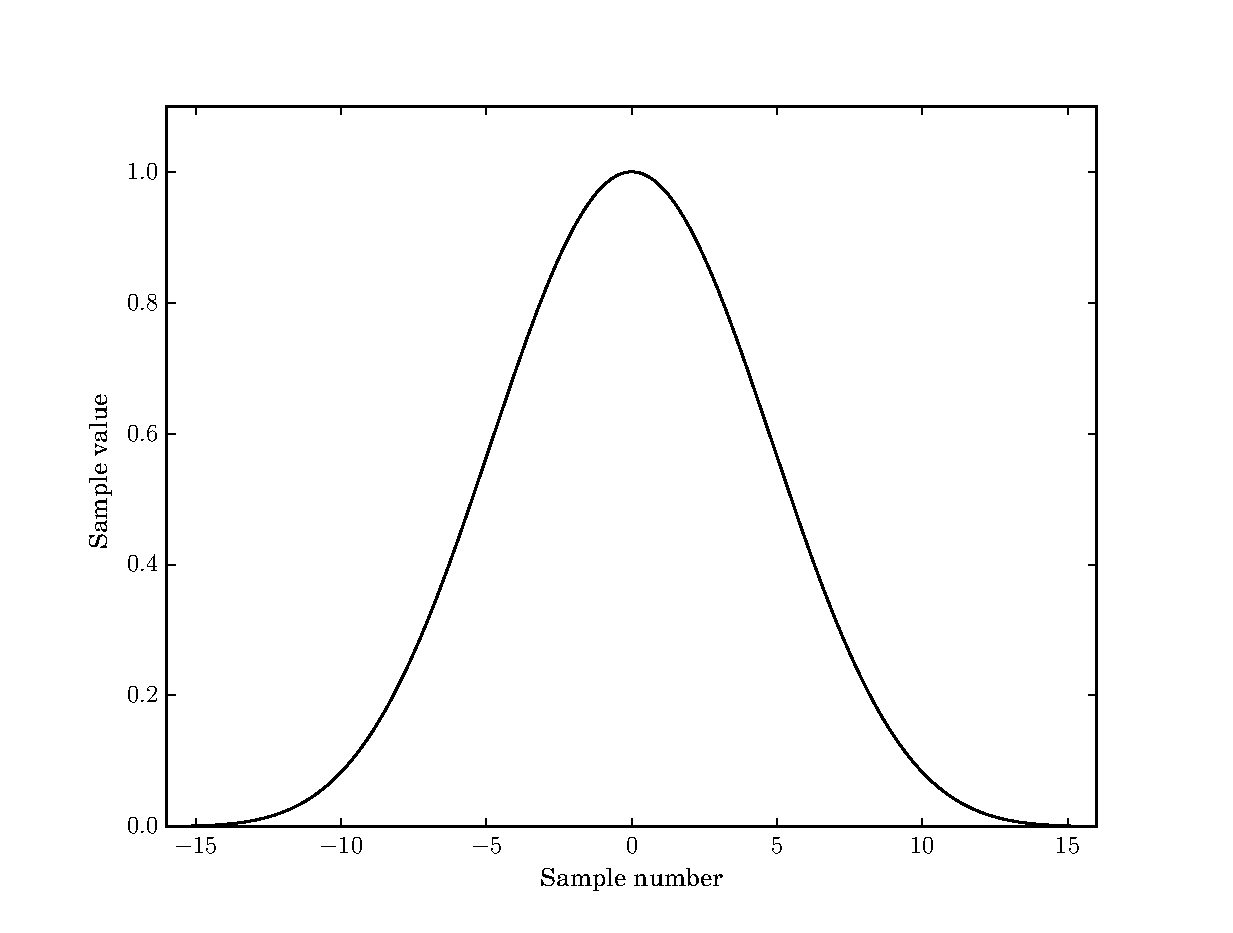
\includegraphics[width=\figwidthscale\textwidth]{plots/c1_blackman_td.eps}
\end{figure}

\begin{figure}[!t]
    \caption{}
    \centering
    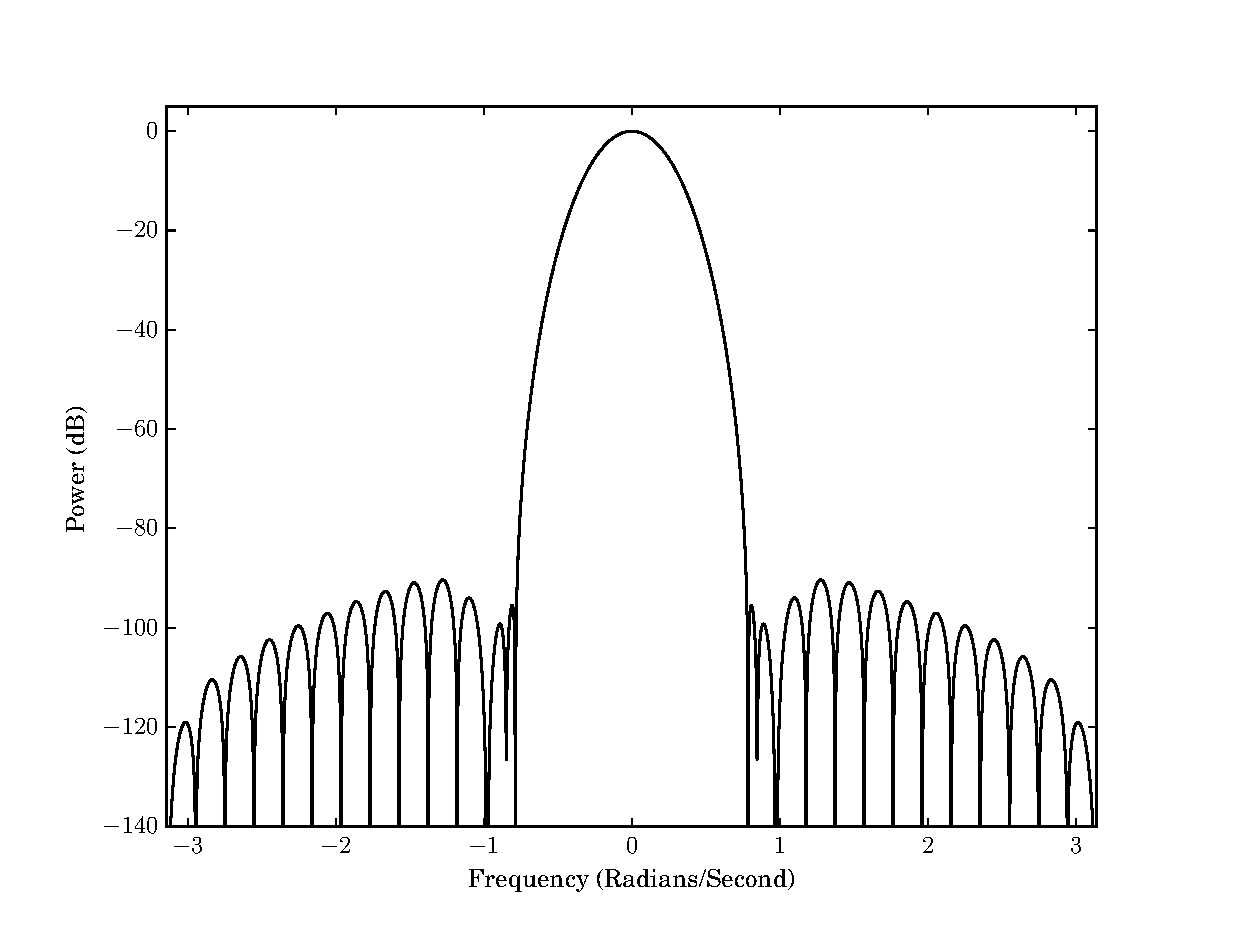
\includegraphics[width=\figwidthscale\textwidth]{plots/c1_blackman_fd.eps}
\end{figure}

\begin{figure}[!t]
    \caption{\label{plot:c1vsminblackmancloseup}}
    \centering
    \includegraphics[width=\figwidthscale\textwidth]{plots/c1_vs_min_blackman_closeup.eps}
\end{figure}

\begin{table}
    \caption{\label{tab:optblackman}}
    \begin{center}
        \begin{tabular}{l c c c c }
            Window & $a_0$ & $a_1$ & $a_2$ & $a_3$ \\
            \hline
            Minimum & 0.35857 & 0.48829 & 0.14128 &
            0.01168 \\
            $\mathcal{C}^{1}$ & 0.35874 & 0.48831 &
            0.14127 & 0.01170
        \end{tabular}
    \end{center}
\end{table}

\begin{table}
    \caption{\label{tab:optvs4termblackman}}
    \begin{center}
        \begin{tabular}{l c c}
            Window & Highest side-lobe level (dB) & 6-dB bandwidth in bins \\
            \hline
            Minimum & -92 & 2.72 \\
            $\mathcal{C}^{1}$ & -90 & 2.66 \\
        \end{tabular}
    \end{center}
\end{table}

As we are dealing with mixtures of sinusoids of small bandwidth, in addition to
the finite time support constraint, we desire atoms whose inner-product is only
significant within a finite bandwidth of interest. To construct these atoms, we
multiply the Fourier atom by the window $w$
\[
    \psi_{\tau,\omega}^{\mathcal{F}_{w}}(n) = w(n-\tau) \exp(-j\omega(n-\tau))
\]

A good overview of different windows and their properties is given in
\cite{harris1978use}. We require that the window be at least
once-differentiable and zero outside of a certain interval, therefore, somewhat
informally, we require
\[
    \lim_{n \rightarrow T} \psi(n) = \psi(T) = 0
\]
The \textit{Hann} window possesses this property
\[
    w_{h}(n) = \begin{cases}
        0.5 + 0.5 \cos \left( \frac{n}{T}\pi \right) & -T \leq n \leq T \\
        0 & \text{otherwise}
    \end{cases}
\]

The Hann window is a member of a class of windows constructed by summing scaled
harmonically related cosine functions, subject to the constraint that the
scaling coefficients sum to 1 so that the window have a value of 1 at $n=0$.
Letting $T=N/2$, where $N$ is the length of the window
\[
    w(n) = \begin{cases}
        \sum_{m=0}^{M-1}a_{m}\cos \left( \frac{2\pi}{N}mn \right) & -\frac{N}{2} \leq n
        \leq \frac{N}{2} \\
        0 & \text{otherwise}
    \end{cases}
\]
With $M=2$ and $a_0 = a_1 = 0.5$, we have the Hann window. The
\textit{Blackman-Harris} family of windows are also sum-of-cosine windows. For
these windows, optimization techniques were used to search for coefficients
giving optimum properties, such as minimum height of the highest side-lobe
(maximum out-of-band rejection) \cite{rabiner1970approach}. The 4-term window
whose coefficients $a$ are listed in Table~\ref{tab:optblackman} has a maximum
side-lobe level of 92 dB, lower than the quantization noise of a 16-bit linear
pulse code modulated signal. This window has a very large main-lobe which means
two sinusoids of similar frequency will be difficult to resolve. Furthermore,
the window has a discontinuity at its boundaries, e.g.,
$w \left( \frac{N}{2} \right) \neq 0$ and is not once-differentiable. In any
case the window is valuble in that it effectively nulls any influence of signals
outside of a bandwidth of interest.

To find a window with properties similar to the 4-term Blackman-Harris window
but without a discontinuity, we solve the optimization problem
\[
        \min||a-\tilde{a}||_2 \\
\]
subject to
\[
        w_{\tilde{a}} \left( \frac{N}{2} \right)
            = w_{\tilde{a}} \left( \frac{-N}{2} \right) = 0
\]
\[
        \sum_{m}^{M-1} a_{m} = 1
\]
where
\[
    w_{\tilde{a}}(n) = \begin{cases}
        \sum_{m=0}^{M-1}\tilde{a}_{m}\cos \left( \frac{2\pi}{N}mn \right) & -\frac{N}{2} \leq n
        \leq \frac{N}{2} \\
        0 & \text{otherwise}
    \end{cases}
\]
The solution $\tilde{a}^{\ast}$ is given in Table~\ref{tab:optblackman} and
plots are given in Figure~\ref{plot:opt_blackman}. This window will be referred
to as the $\mathcal{C}^{1}$ 4-Term Blackman-Harris window. Some figures of merit
for the two windows are compared in Table~\ref{tab:optvs4termblackman} in a similar
fashion to \cite{harris1978use}. We see
that the $\mathcal{C}^{1}$ 4-Term Blackman-Harris window is not too different
from the Minimum 4-term Blackman-Harris window, but has the additional
desirable property of differentiability everywhere in its domain. A comparison
of the windows's endpoints is presented in
Figure~\ref{plot:c1vsminblackmancloseup}.

\section{Partial Tracking\label{sec:partialtracking}}

In Section~\ref{sec:mqfmfromphase} we discussed how to determine reasonable
values for the coefficients of a cubic phase polynomial by using the frequency,
phase and time difference of two local maxima in the DTSTFT. In this section we
discuss possible ways of determining which local maxima are connected. This is
referred to as \textit{peak matching} \cite{mcaulay1986speech}
or \textit{partial tracking} \cite{smith1987parshl} \cite{depalle1993tracking}.

\subsection{A Greedy Method}

The original method of connecting peaks in the spectrogram is from
\cite{mcaulay1986speech}. This method is simple and fast but, as we will see,
can be sensitive to spurious peaks.

Typically the DTSTFT is computed for a block of contiguous samples, called a
\textit{frame} and these frames are computed every $H$ samples, $H$ being the
\textit{hop-size}. Consider the parameters of local maxima in adjacent frames
$h$ and $h+1$ with $M$ maxima in frame $h$ and $N$ maxima in frame $h+1$. In
\cite{mcaulay1986speech}  the parameters are the instantaneous amplitude, phase
and frequency and are indexed by frequency as $\omega_0^{h}, \dotsc,
\omega_{M-1}^{h}$ and $\omega_0^{h+1}, \dotsc, \omega_{N-1}^{h+1}$, but here we
allow for an arbitrary set of parameters $\theta_0^{h}, \dotsc,
\theta_{M-1}^{h}$ and $\theta_0^{h+1}, \dotsc,
\theta_{N-1}^{h+1}$, such as the coefficients of a phase polynomial. Define a
distance function $\mathcal{D} \left( \theta_{i},\theta_{j} \right)$ that computes the
similarity between two sets of parameters. We will now consider a method that
finds $L$ pairs of parameters that are closest.

We compute the cost matrix $\boldsymbol{C}$
\[
    \boldsymbol{C} = \theta^{h} \otimes_{\mathcal{D}} \theta^{h+1}
\]
so that the $i$th row and $j$th column contain $C_{i,j} = \mathcal{D} \left(
\theta_{i}^{h},\theta_{j}^{h+1} \right)$.  For each $l \in \left[0 \dotsc L-1
\right]$, find the indices $i_{l}$ and $j_{l}$ corresponding to the shortest
distance, then remove the $i_{l}$th row and $j_{l}$th column from consideration
and continue until $L$ pairs have been determined or the distances exceed some
threshold $\Delta$. This is summarized in Algorithm~\ref{alg:mq_peak_match}

\begin{algorithm}[H]
    \caption{\label{alg:mq_peak_match}}
    \KwIn{the cost matrix $\boldsymbol{C}$}
    \KwOut{$L$ index pairs $\Gamma_{i}$ and $\Gamma_{j}$}
    $\Gamma_{i} \leftarrow \varnothing$\;
    $\Gamma_{j} \leftarrow \varnothing$\;
    \For{$l \leftarrow 0$ to $L-1$}{
        $\D i_{l},j_{l}=\argmin_{i \in \left[ 0,\dotsc,M-1 \right] \setminus
        \Gamma_{i}, j \in \left[ 0,\dotsc,M-1 \right] \setminus \Gamma_{j}}
        C_{i,j}$\;
        \If{$ C_{i_{l},j_{l}} > \Delta$}{
            \KwRet{$\Gamma_{i},\Gamma_{j}$}
        }
        $\Gamma_{i} \leftarrow \Gamma{i} \cup i_{l}$\;
        $\Gamma_{j} \leftarrow \Gamma{i} \cup j_{l}$\;
    }
    \KwRet{$\Gamma_{i},\Gamma_{j}$}
\end{algorithm}

This is a greedy algorithm because on every iteration the smallest cost is
identified and its indices are removed from consideration. Perhaps choosing a
slightly higher cost in one iteration would allow smaller costs to be chosen in
successive iterations. This algorithm does not allow for that. In other terms,
the algorithm does not find a set of pairs that represent a globally minimal sum of
costs.
Another drawback of the algorithm is that it only works between two sucessive
frames. The cost function could be extended to consider $K$ sets of parameters,
constructing an $K$-dimensional tensor instead of a matrix, but assuming equal
numbers of parameter sets in all frames, the search space would grow
exponentially with $K$. Nevertheless, the method is simple to implement,
computationally negligble when $K$ is small, and works well with a variety of
signals encountered in audio \cite{mcaulay1986speech} \cite{smith1987parshl}.

\subsection{An Optimal Method \label{sec:lppathsearch}}

There is a way to find a set of paths over multiple frames ($K > 2$) having the
lowest total cost if
we restrict the search to exactly $L$ paths. Instead of indexing parameters by
their frame number $h$, we make $h$ part of the parameter set so that it can be
used by the distance function $\mathcal{D}$. Assume that over $K$ frames there
are $M$ total parameter sets. We define the vector $\boldsymbol{c} \in \mathbb{R}^{M^2}$
where the entry $\boldsymbol{c}_{i + Mj} = \mathcal{D} \left( \theta_{i}, \theta_{j}
\right)$. If we have a set of connections $\Gamma_{i,j}$ we can calculate the
total cost of these connections by defining the vector
\[
    \boldsymbol{x}_{i + Mj} = \begin{cases}
        1 & \text{there is a connection between }i\text{ and }j\\
        0 & \text{otherwise}
    \end{cases}
\]
and then forming the inner product
\[
    c_{\text{total}}=\left\langle \boldsymbol{c},\boldsymbol{x} \right\rangle
\]
Note that a node cannot be connected to itself. The question is how to find
$\boldsymbol{x}^{\ast}$ so that $c_{\text{total}}$ is minimized. If no
constraints are placed on $\boldsymbol{x}$, the solution is trivial, but not
useful. How do we constrain $\boldsymbol{x}$ to give us a solution to the
partial tracking problem? Let us consider an example.

In Figure~\ref{plot:simple_graph} we have an example of a simple graph or
lattice. The numbers are indices of nodes in the graph and the possible
connections between them are indicated by lines, or \textit{edges}. We would
like to find the two shortest paths based on different criteria. In
Figure~\ref{plot:simple_graph_greedy_paths} we find the paths using an algorithm
similar to Algorithm~\ref{alg:mq_peak_match} but search instead over a tensor of
distances $C \in \mathbb{R}^{3 \times 4 \times 2}$ whose entry $C_{i,j,h}$
represents the cost of travelling on the path connecting the $i$th node in layer
0, the $j$th node in layer 1 and the $h$th node in layer 2. This is the greedy
method of searching for the best paths whose optimality criterion is to find the
set of best paths containing the absolute best path. We see in
Figure~\ref{plot:simple_graph_greedy_paths} that the absolute shortest path, $1
\rightarrow 4 \rightarrow 8$, is discovered, followed by the second shortest
path not using the nodes of the first path.

\begin{figure}[!t]
    \caption{\label{plot:simple_graph}}
    \centering
    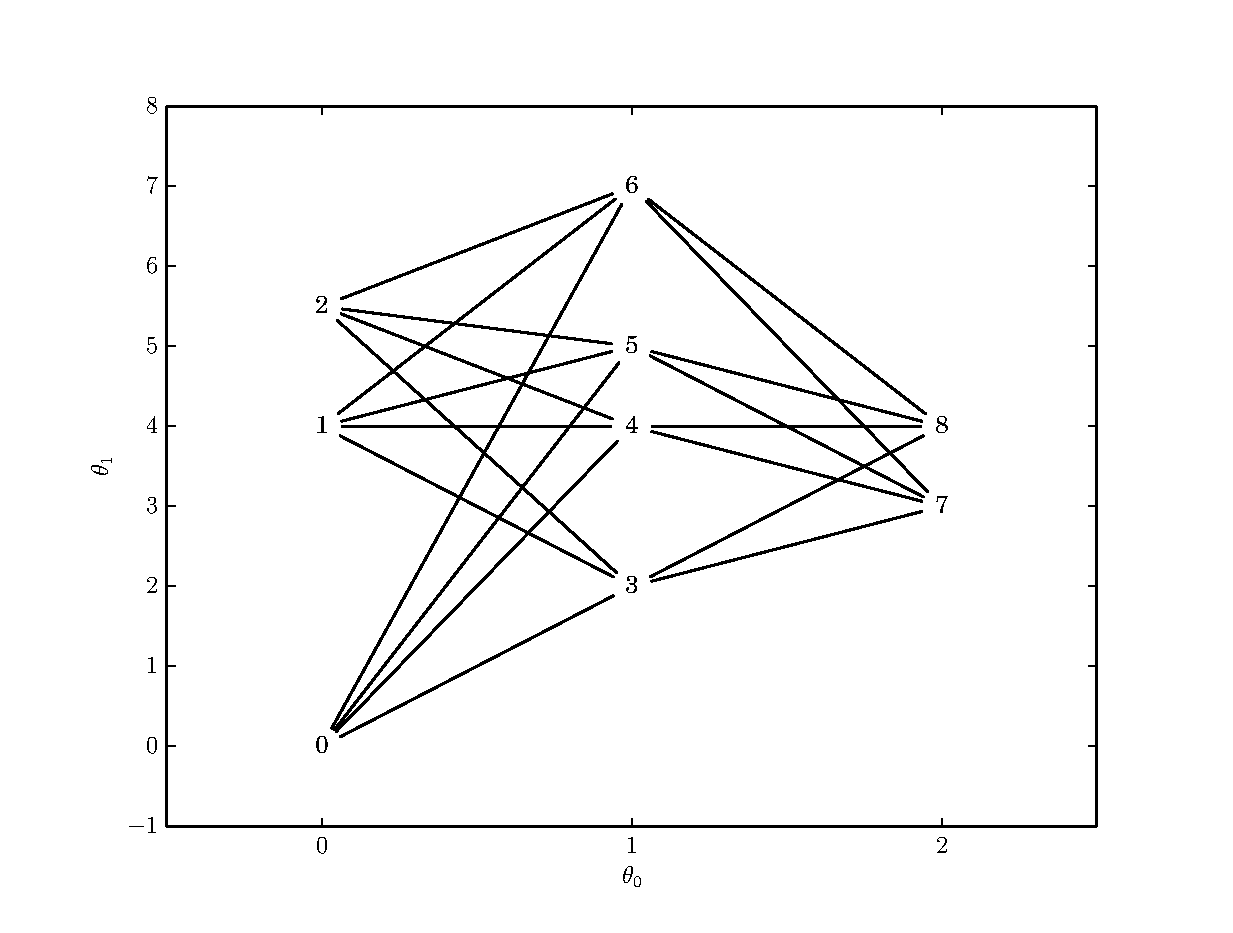
\includegraphics[width=\figwidthscale\textwidth]{plots/small_graph_ex.eps}
\end{figure}

\begin{figure}[!t]
    \caption{\label{plot:simple_graph_greedy_paths}}
    \centering
    \includegraphics[width=\figwidthscale\textwidth]{plots/small_graph_ex_greedy_paths.eps}
\end{figure}

To find a set of paths minimizing the total cost, we instead search for total
solutions $\boldsymbol{x}$ that describe all paths in the graph. Assume for now
that we can guarantee that the entries of $\boldsymbol{x}$ will be either 0 or
1. To find a set of constraints for our search, we consider the structure of a
valid solution $\boldsymbol{x}^{\ast}$. To maintain that paths not overlap, a
valid solution's nodes are only allowed to have one edge entering ---
coming from a node in a previous frame --- and one edge leaving
--- going to a node in a successive frame. To translate this into a
constraint, consider the node $i$ and its possible $R$ successive connecting
nodes $j_{0} \dotsc j_{R-1}$. Define the vector
\[
    a^{\text{s},i}_{i + Mj_{r}} = \begin{cases}
        1 & \forall j_{r} \in \left[ j_{0} \dotsc j_{R-1} \right] \\
        0 & \text{otherwise}
    \end{cases}
\]
As all the entries of $\boldsymbol{x}$ are either 0 or 1, we have
\[
    0 \leq \left\langle \boldsymbol{a}^{\text{s},i}, \boldsymbol{x} \right\rangle \leq 1
\]
so we can make this a constraint to ensure that a node has at most one path
leaving. Similarly, if we consider the node $j$ and its possible R previous connecting
nodes $i_{0} \dotsc i_{R-1}$, the vector
\[
    a^{\text{p},j}_{i_{r} + Mj} \begin{cases}
        1 & \forall i_{r} \in \left[ i_{0} \dotsc i_{R-1} \right] \\
        0 & \text{otherwise}
    \end{cases}
\]
constrains that node $j$ have only one path entering through the constraint
\[
    0 \leq \left\langle \boldsymbol{a}^{\text{p},j} , \boldsymbol{x} \right\rangle \leq 1
\]
A node on a path will also have an edge entering and an edge leaving. To
translate this into a constraint, we define a vector that counts the number of
edges entering a node and subtracts then the number of edges leaving a node. The
result should always be 0 for an equal number of edges entering and exiting a
node. If $r$ is the index of the node considered, the vector is simply
\[
    \boldsymbol{a}^{\text{b},r} = \boldsymbol{a}^{\text{p},r} -
    \boldsymbol{a}^{\text{s},r}
\]
and the constraint
\[
    \left\langle \boldsymbol{a}^{\text{b},r}, \boldsymbol{x} \right\rangle = 0
\]
Finally we want to constrain that there be only $L$ paths. We do this by
noticing that if this is true, there will be $L$ edges between frames $h$ and
$h+1$. We constrain the number of paths going from edges
$\Gamma_{h}$ in frame $h$ to $\Gamma_{h+1}$ by forming the vector
\[
    \boldsymbol{a}^{\text{c},h} = \sum_{j \in \Gamma_{h}}
    \boldsymbol{a}^{\text{s},j}
\]
and asserting the constraint
\[
    \left\langle \boldsymbol{a}^{\text{c},h} , \boldsymbol{x} \right\rangle = L
\]
The length of $\boldsymbol{x}$ is $M^{2}$ so the total size of all the
constraints is not insignificant, but most entries in the constraint vectors will
be 0 and therefore the resulting constraint matrices very sparse, so sparse
linear algebra routines can be used in computations. Furthermore, the
$\boldsymbol{a}^{b}$ and $\boldsymbol{a}^{c}$ constraints are derived from
$\boldsymbol{a}^{p}$ and $\boldsymbol{a}^{s}$, so only the latter need to be
stored.

The complete \textit{linear program (LP)} solving the $L$ shortest paths problem is then
\begin{samepage}
\[
    \min_{\boldsymbol{x}} \left\langle \boldsymbol{c}, \boldsymbol{x} \right\rangle
\]
subject to
\[
    \boldsymbol{0} \leq
    \begin{bmatrix}
        \boldsymbol{A}_{\text{s}} \\
        \boldsymbol{A}_{\text{p}}
    \end{bmatrix} \boldsymbol{x}
    \leq \boldsymbol{1}
\]
\[
    \begin{bmatrix}
        \boldsymbol{A}_{\text{b}} \\
        \boldsymbol{A}_{\text{c}}
    \end{bmatrix}
    \boldsymbol{x}
    =
    \begin{bmatrix}
        \boldsymbol{0} \\
        L\boldsymbol{1}
    \end{bmatrix}
\]
\[
    \boldsymbol{0} \leq \boldsymbol{x} \leq \boldsymbol{1}
\]
\end{samepage}
where $\boldsymbol{A}_{\text{s}}$ is the matrix with
$\boldsymbol{a}^{\text{s},m}$ as its rows for $m \in [0 \dotsc M-1]$ and
$\boldsymbol{A}_{\text{p}}$ is the matrix with $\boldsymbol{a}^{\text{p},m}$ as
its rows, etc.

\begin{figure}[!t]
    \caption{\label{plot:simple_graph_lp_paths}}
    \centering
    \includegraphics[width=\figwidthscale\textwidth]{plots/small_graph_ex_lp_paths.eps}
\end{figure}

The solution of the two best paths using the LP formulation
is shown in Figure~\ref{plot:simple_graph_lp_paths} and a comparison of the
total costs is shown in Table~\ref{tab:greedy_lp_cost_compare}

\begin{table}
    \caption{\label{tab:greedy_lp_cost_compare} Comparison of total costs}
    \begin{center}
        \begin{tabular}{c c}
            Greedy & LP \\
            \hline
            \input{plots/small_graph_ex_greedy_cost.txt} &
            \input{plots/small_graph_ex_lp_cost.txt} \\
        \end{tabular}
    \end{center}
\end{table}

The LP formulation is based on a multiple object tracking algorithm for video
\cite{jiang2007linear}. A proof that the solution $\boldsymbol{x}^{\ast}$ will
have entries equal to either $0$ or $1$ can be found in
\cite[p.~167]{parker1988discrete}. The theoretical computational complexity of
the linear program is polynomial in the number of variables, see
\cite{karmarkar1984new} for a proof and the demonstration of a fast algorithm
for finding its solution. In practice, to extract paths from the solution, we do
not test equality with $0$ or $1$ but rather test if the solution vector's
values are greather than some threshold. This may mean that suboptimal solutions
may still be close enough. The tolerance of the solutions to suboptimality
should be investigated, as if they are tolerant, fewer iterations of a
barrier-based algorithm would be required to solve the problem. More information
on linear programming and optimization in general can be found in
\cite{boyd2004convex}.

It should be noted that in the special case that only 1 shortest path is
searched an algorithm exists that requires on the order of $N^{2}T$ calculations
\cite{rabiner1989tutorial} where $N$ is the number of nodes in each frame and
$T$ is the number of frames (assuming the same number of nodes in each frame):
this algorithm is known as the Viterbi algorithm \cite{forney1973viterbi}.

The LP formulation of the $L$-best paths problem gives results equivalent to the
solution to the $L$-best paths problem proposed in \cite{wolf1989finding}. The
complexity of our algorithm is different from that in this paper.  Assuming we
use the algorithm in \cite{karmarkar1984new} to solve the LP, our program has a
complexity of $O(M^{7}B^{2})$ where $M$ is the number of nodes (parameter sets)
and $B$ is the number of bits used to represent each number in the input. The
complexity of the algorithm in \cite{wolf1989finding} is equivalent to the
Viterbi algorithm for finding the single best path through a trellis whose $h$th
frame has $\binom{N_{h}}{L}\binom{N_{h+1}}{L}L!$ connections where $N_{h}$ and
$N_{h+1}$ are the number of nodes in two consecutive frames of the original
lattice. Therefore, assuming a constant number $N$ of nodes in each frame, its
complexity is $O((\binom{N}{L}^{2}L!)^{2}T)$. If there are few nodes in each
frame and a small number of paths are searched, the Viterbi formulation is
superior as its complexity increases linearly with the number of frames in the
lattice. On the other hand, if each frame has a large number of nodes or many
paths are searched, the LP formulation is superior.  Informally we have found
this to agree with reality --- both algorithms were tried when producing the
figures in Section~\ref{sec:mq_lp_compare_chirp}.  Indeed the Viterbi
formulation took prohibitvely long to compute when many paths were desired, as
did the LP when many frames were considered.

\subsection{Partial paths on example signal\label{sec:mq_lp_compare_chirp}}

We compare the greedy and LP based methods for peak matching on a synthetic
signal. The signal is composed of $K=6$ chirps of constant amplitude, the $k$th
chirp $s$ at sample $n$ described by the equation
\[
    s_{k}(n) = \exp(j(\phi_{k} + \omega_{k}n +
    \frac{1}{2} \psi_{k} n^{2}))
\]
The parameters for the 6 chirps are presented in
Table~\ref{tab:ptrackexamplechirpparams}.
\begin{table}
    \caption{Parameters of $k$th chirp. $f_{0}$ and $f_{1}$ are the initial and
    final frequncy of the chirp in Hz. \label{tab:ptrackexamplechirpparams}}
    \begin{center}
        \begin{tabular}{l c c c c c}
            $k$ & $\phi_{k}$ & $\omega_{k}$ & $\psi_{k}$ & $f_{0}$ & $f_{1}$ \\
            \hline
            \input{plots/mq_lp_compare_chirp_params.txt}
        \end{tabular}
    \end{center}
\end{table}

Two 1 second long signals are synthesized at a sampling rate of 16000 Hz, the
first with chrips 0--2, the second with chirps 3--5. We add
Gaussian distributed white noise at several SNR to evalute the technique in the
presence of noise.

A spectrogram of each signal is computed with an analysis window length of 1024
samples and a hop-size $H$ of 256 samples. Local maxima are searched in 150 Hz
wide bands spaced 75 Hz apart. A local maximum is only accepted if its amplitude
is greater than -20 dB. At each local maximum the DDM is used to estimate the
local chirp parameters, the $i$th set of parameters in frame $h$ denoted
$\theta_{i}^{h} = \left\{ \phi_{i}^{h} , \omega_{i}^{h} , \psi_{i}^{h}
\right\}$. The results of the analyses of both signals are lumped together and
it is on this lumped data that we perform partial tracking.

We search for partial tracks using both the greedy and LP strategies. Both
algorithms use the distance metric $\mathcal{D}$ between two parameters sets:
\[
    \mathcal{D} \left( \theta_{i}^{h},
    \theta_{j,}^{h+1} \right) = \left( \omega_{i}^{h} +
    \psi_{i}^{h} H - \omega_{j}^{h+1} \right)
\]
Which is the error in predicting $j$th frequency in frame $h+1$ from the $i$th
parameters in frame $h$. For the greedy method, the search for partial paths is
restricted to one frame ahead like in \cite{mcaulay1986speech}. For the LP
method, to keep the computation time reasonable, we search over 6 frames for 6
best paths\footnote{The number of paths does not affect the computation time.}.
To maintain connected paths, the search on the next frames uses the end nodes of
the last search as starting points. For both methods, the search is restricted
to nodes between frequencies 250 to 2250 Hz.

\begin{figure}[!t]
    %\centering
    \centering
    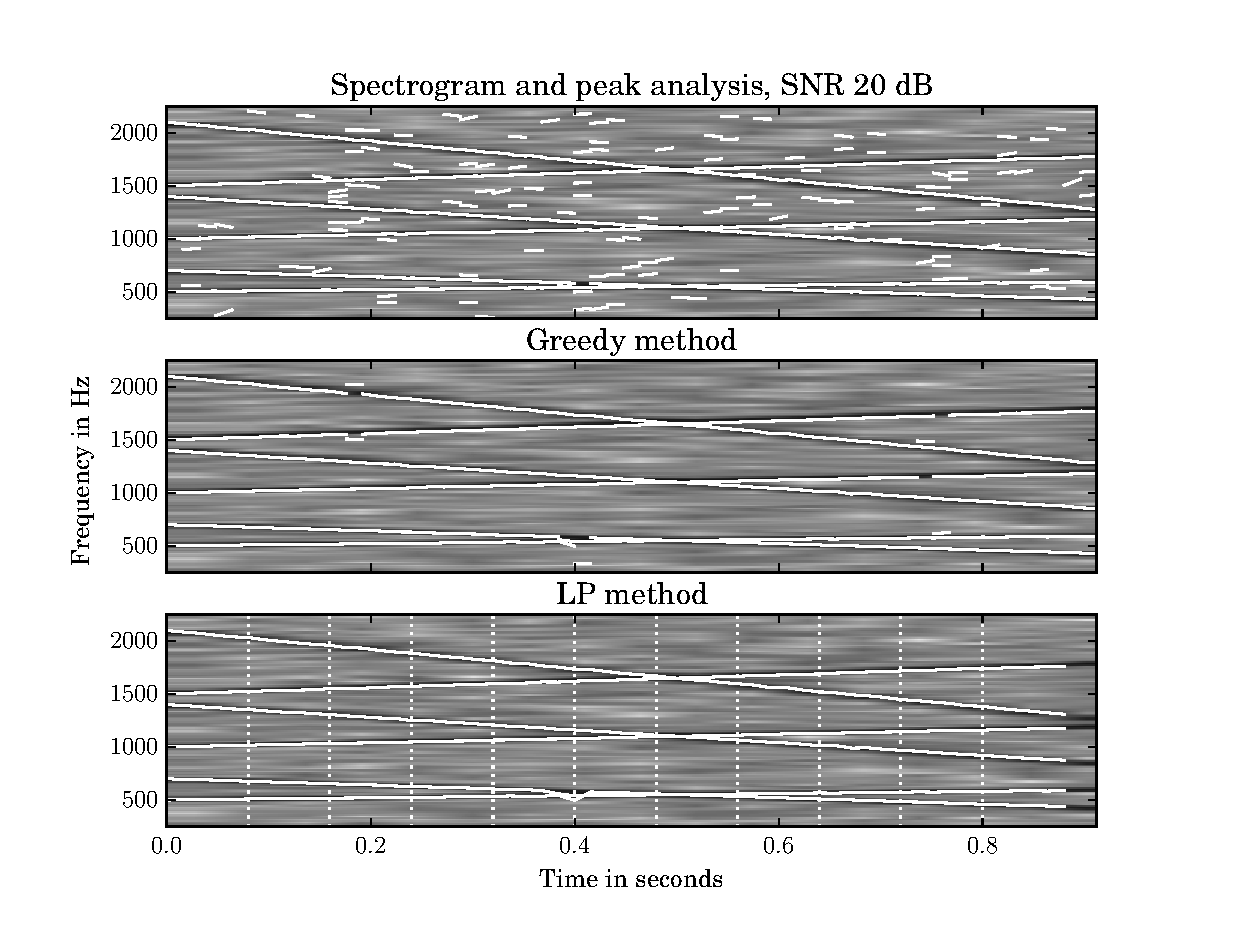
\includegraphics[width=\figwidthscale\textwidth]{plots/mq_lp_compare_chirp_20.eps}
    \caption{ Line-segments representing the discovered partial paths.
    \label{plot:mq_lp_compare_chirp_20}}
\end{figure}
\begin{figure}[!t]
    %\centering
    \centering
    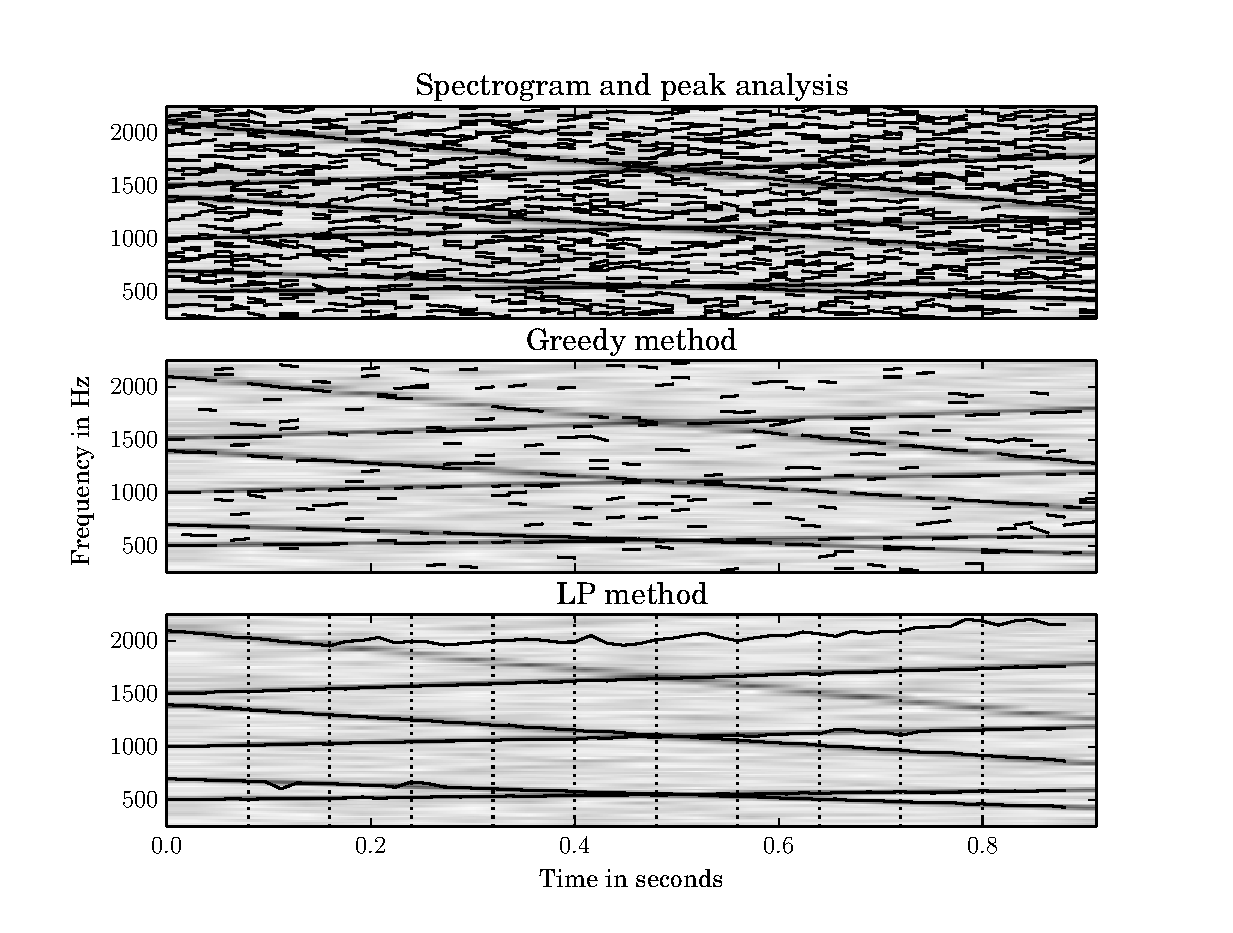
\includegraphics[width=\figwidthscale\textwidth]{plots/mq_lp_compare_chirp_15.eps}
    \caption{ Line-segments representing the discovered partial paths.
    \label{plot:mq_lp_compare_chirp_15}}
\end{figure}
\begin{figure}[!t]
    %\centering
    \centering
    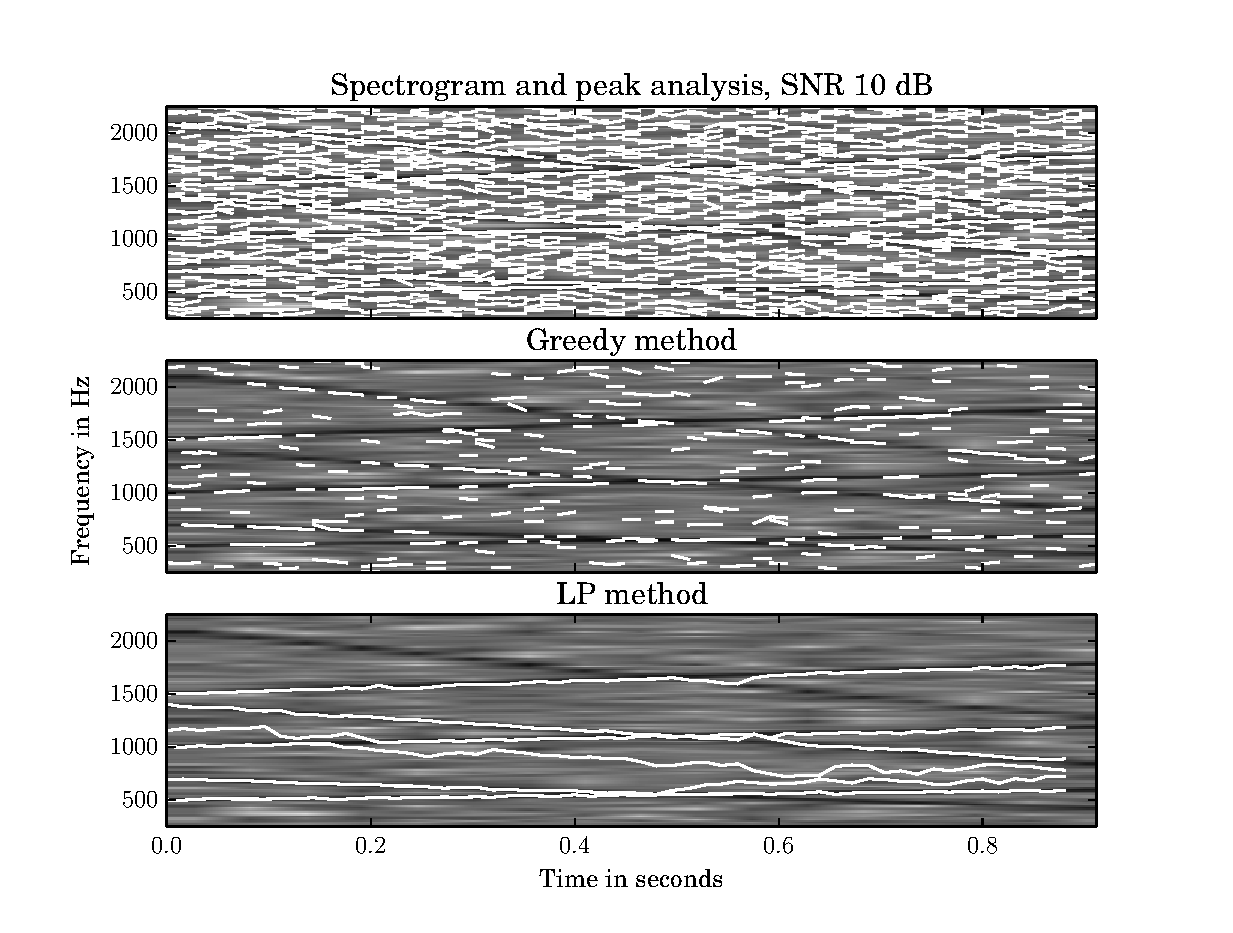
\includegraphics[width=\figwidthscale\textwidth]{plots/mq_lp_compare_chirp_10.eps}
    \caption{ Line-segments representing the discovered partial paths.
    \label{plot:mq_lp_compare_chirp_10}}
\end{figure}
%\begin{figure}[!t]
%    %\centering
%    \centering
%    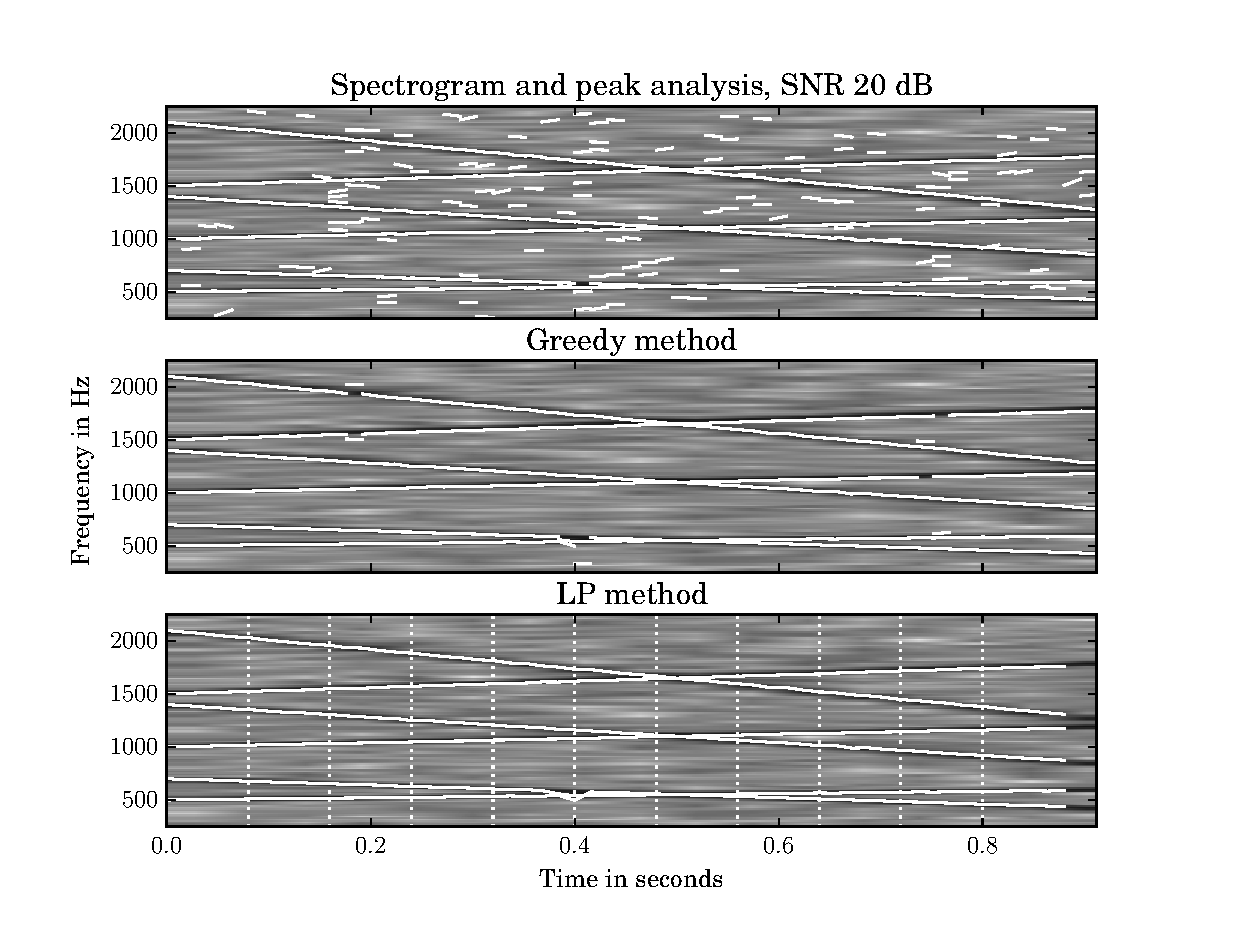
\includegraphics[width=\figwidthscale\textwidth]{plots/mq_lp_compare_chirp_20.eps}
%    \caption{ Line-segments representing the discovered partial paths.
%    \label{plot:mq_lp_compare_chirp_hint20}}
%\end{figure}
%\begin{figure}[!t]
%    %\centering
%    \centering
%    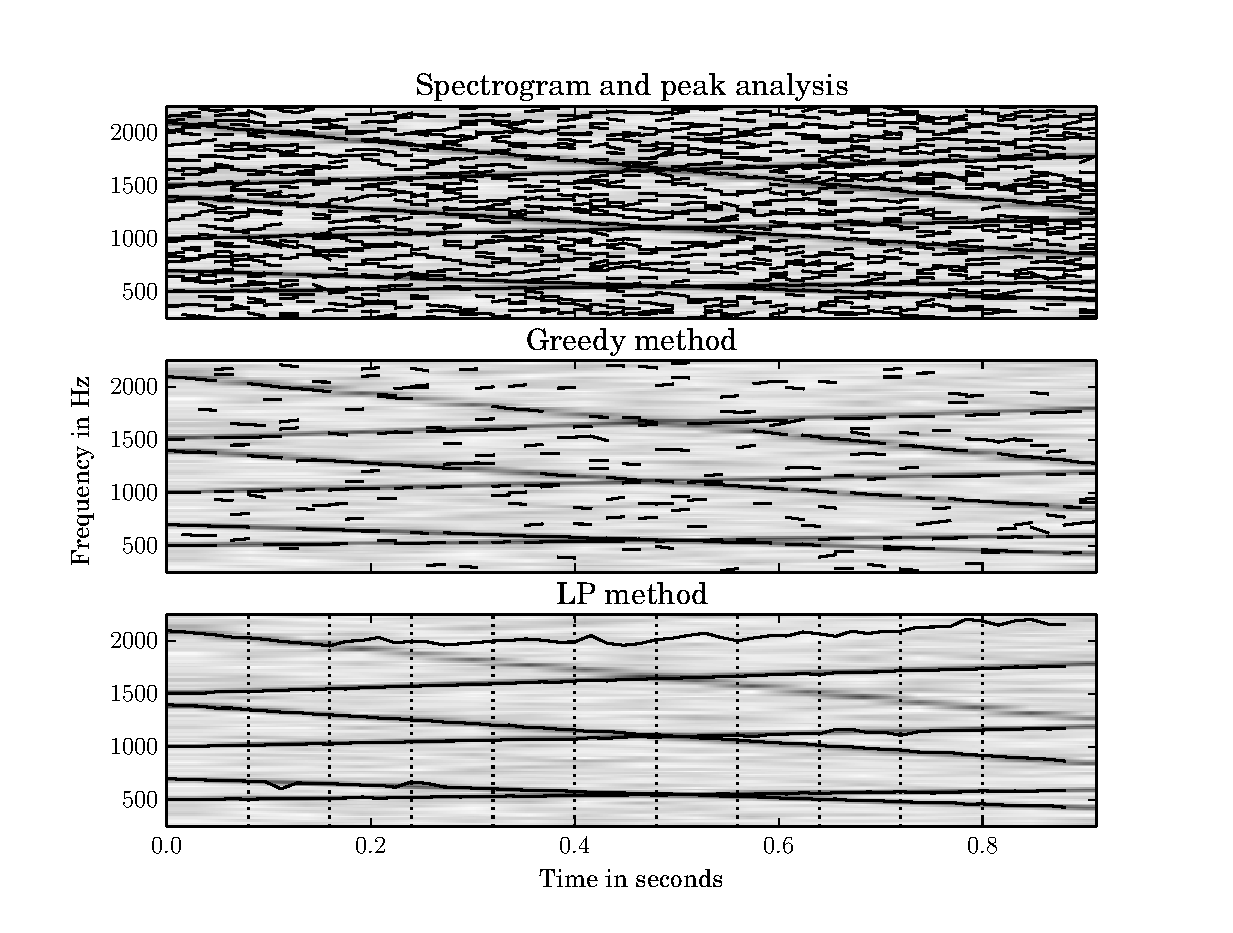
\includegraphics[width=\figwidthscale\textwidth]{plots/mq_lp_compare_chirp_15.eps}
%    \caption{ Line-segments representing the discovered partial paths.
%    \label{plot:mq_lp_compare_chirp_hint15}}
%\end{figure}
Figures~\ref{plot:mq_lp_compare_chirp_10},~\ref{plot:mq_lp_compare_chirp_15}~and~\ref{plot:mq_lp_compare_chirp_20}
show discovered partial trajectories for signals with SNR of 10, 15 and 20 dB
respectively. We can see that while the greedy method begins to perform poorly
at an SNR of 15dB, the LP method still gives plausible partial trajectories for
SNRs of 10 and 15 dB. At lower signal to noise ratios, the LP formulation gives
some paths that do not correspond to an underlying partial. These could be filtered
out by examining the cost of these paths and comparing them to the costs of the
others. Those that deviate from a mean cost more than a certain amount should be
rejected. This is the strategy used in Chapter~\ref{chap:decaysep} and
illustrated in Figure~\ref{plot:acgtra3xylofs4costlengththresh}.

But why did the LP discover a path not present in the underlying signal? This is
due to the cost function, which finds a path with minimum prediction error in
using the frequency and frequency slope coefficients of one node to predict
another node's frequency coefficient. When there are many nodes in the original
analysis it is not surprising that some unexpected path exists.  An attribute of
these erroneous paths is that they are not smooth. To deter the algorithm from
finding such paths, regularization could be used like in
Section~\ref{sec:mqfmfromphase} that minimizes the integral of the squared
estimate of the path's second derivative. More on regularization in optimization
can be found in \cite[ch.~6.3]{boyd2004convex}.
% Could also try and maximize smoothness of trajectories by adding second order
% differences as a cost.

%As a further test, we give the algorithms a hint by
%removing all spurious data-points from the first frame. We can see in
%Figures~\ref{plot:mq_lp_compare_chirp_hint15}~and~\ref{plot:mq_lp_compare_chirp_hint20}
%that this improves the results for the LP method.

\section{Classification}

If data-points consist of more than two dimensions (say $p$), it becomes
burdensome to try and find the single best or two best dimensions on which to
examine for grouping. If we consider variables on each of the dimensions that
take on the data-point's corresponding values, we are interested in the
variables that capture most of the data-points's variance. In turns out we can
determine a linear transformation of our original dataset giving $p$ variables
and their $p$ variances such that the resulting variable with the highest
variance will have the maximum variance acheivable, under some constraints that
will be explained shortly. 

\subsection{Principal components analysis (PCA)}

The following development is based on \cite{jolliffe2002principal}. Say we have
a set $\left\{ \boldsymbol{x} \right\}$ of data-points and their covariance
matrix $\boldsymbol{S}$. A linear function of $\boldsymbol{x}$,
$f_1(\boldsymbol{x})=\boldsymbol{a}_{1}^{T}\boldsymbol{x}$ has variance
$\sigma_{\boldsymbol{a}_{1}^{T}\boldsymbol{x}}=\boldsymbol{a}_{1}^{T}\boldsymbol{S}\boldsymbol{a}_{1}$.
Therefore, we desire a vector $a$ that maximizes
$\sigma_{\boldsymbol{a}_{1}^{T}\boldsymbol{x}}$. We can find this via the program
\[
        \max \boldsymbol{a}_{1}^{T}\boldsymbol{S}\boldsymbol{a}_{1}
\]
subject to
\[
    \boldsymbol{a}_{1}^{T}\boldsymbol{S}\boldsymbol{a}_{1}=1
\]
(to obtain a bounded solution).

The resulting function of $\boldsymbol{x}$,
$f_1(\boldsymbol{x})=\boldsymbol{a}_{1}^{\ast T}\boldsymbol{x}$ is called the first
\textit{principal component}. The second principal component
$f_2(\boldsymbol{x})=\boldsymbol{a}_{2}^{\ast T}\boldsymbol{x}$ is found similary
to the first, except with the additional constraint that it be uncorrelated
(orthogonal) to the first component, i.e.,
$\boldsymbol{a}_{2}^{\ast T}\boldsymbol{a}_{1}=0$, and the third is found by
requiring orthognality with the first two principal components, etc.

The principal components (PCs) now allow us to examine for grouping more easily as the
total variance of the dataset has been captured in the first few principal component
variables. These transformed data-points can now be classified using a
classification algorithm.

Before we continue describing classification techniques we will briefly discuss
the nature of our classification problem. If accurate and consistent
measurements of data-points can be made, and a large enough sample of
data-points is available to train a model, then to predict the classification of
new points, a function $g=\hat{h} \left( \boldsymbol{x} \right)$ is postulated,
giving the classification $g$ of a data-point $\boldsymbol{x}$. For example, if
there are only two classes, we might postulate a linear
classifier
\[
    \hat{h}(\boldsymbol{x}) = \begin{cases}
        0 \text{ if } \boldsymbol{\beta}^{T}\boldsymbol{x} > c \\
        1 \text{ if } \boldsymbol{\beta}^{T}\boldsymbol{x} < c
    \end{cases}
\]
where 0 and 1 indicate membership in class 0 or 1. Techniques for choosing
$\hat{h}$ are discussed in \ref{friedman2001elements} and often require data on
which to ``train'' a classifier, i.e., determine a function $\hat{h}$ that
classifies well a dataset with known classifications.  Here we do not have a
sample dataset because of the large number of possible situations and the
difficulty of consistently estimating underlying model parameters (see, for
example, Section~\ref{sec:mq_lp_compare_chirp}). As training to find a suitable
$\hat{h}$ is not possible, we propose \textit{kernels} that reflect the
hypothesized underlying structure of the distribution of $\boldsymbol{x}$. To
elaborate, we may observe that the classification of a
point is indicated by its nearness to other points in the same class, i.e., its
membership to a cluster. The proposed kernel is a parameterized model of a
cluster, whose parameters we can adjust until they fit the observed data well.
We then choose the kernel that best explains the data to indicate what class
these data are in. The following section describes a technique using normal
distributions as kernels, which is the technique used in later experiments.

\subsection{Gaussian Mixture Models (GMM) \label{sec:gmm}}

Consider the data-points $\boldsymbol{X}$ as realizations of the vector Gaussian
distributed random variable $X$. With a large enough sample and a small enough
covariance, we will observe realizations of $X$ as a cluster with some mean
(centre point) $\boldsymbol{\mu}$ and a shape described by the covariance matrix
$\boldsymbol{\Sigma}$. If we observe multiple clusters this might imply that
there are $P$ different distributions each with mean $\boldsymbol{\mu}_p$ and
covariance matrix $\boldsymbol{\Sigma}_p$ and on each iteration one is chosen
with probability $w_p$. With $N$ observations $\boldsymbol{x}_{n}$ we can
estimate, via maximum likelihood, the $P$ sets of parameters using a form of the
\textit{expectation maximization (EM)} algorithm \cite{moon1996expectation},
\cite{dempster1977maximum}, which is an algorithm suitable for estimating
missing data from known ones. First, define
\[
    \mathrm{p} \left( \boldsymbol{x}_{n} | p \right)
    =
    \ddfrac{
        \mathcal{N} \left( \boldsymbol{x}_{n}; \boldsymbol{\mu}^{k}_{p} ,
        \boldsymbol{\Sigma}^{k}_{p} \right) w^{k}_{p}
    }{
        \sum_{l=1}^{P}
        \mathcal{N} \left( \boldsymbol{x}_{n}; \boldsymbol{\mu}^{k}_{l} ,
        \boldsymbol{\Sigma}^{k}_{l} \right) w^{k}_{l}
    }
\]
the probability that $\boldsymbol{x}_n$ given distribution $p$ (see
Appendix~\ref{apdx:gaussian_dist} for the definition of $\mathcal{N} \left(
\boldsymbol{x} ; \boldsymbol{\mu}^{k} , \boldsymbol{\Sigma}^{k} \right)$). The superscript $k$
indicates the value of this parameter on iteration $k$. To update $w^{k}_p$:
\[
    w^{k+1}_p = \frac{1}{N} \sum_{n=1}^{N} \mathrm{p} \left( \boldsymbol{x}_n |
    p \right)
\]
which means intuitively that the probability of a data-point having been
generated by distribution $p$ is the average probability of observing any
$\boldsymbol{x}_n$ given $p$. To update $\boldsymbol{\mu}^{k+1}_p$:
\[
    \boldsymbol{\mu}^{k+1}_p
    =
    \ddfrac{\sum_{n=1}^{N} \mathrm{p} \left( \boldsymbol{x}_n |
    p \right) \boldsymbol{x}_n }{\sum_{n=1}^{N} \mathrm{p} \left( \boldsymbol{x}_n |
    p \right)}
\]
which is a weighted mean of all the data-points. Those less likely for a
given $p$ will weight the mean less and vice versa. A similar computation is
made for $\boldsymbol{\Sigma}^{k+1}_p$:
\[
    \boldsymbol{\Sigma}^{k+1}_p
    =
    \ddfrac{\sum_{n=1}^{N} \mathrm{p} \left( \boldsymbol{x}_n | p \right)
        \left( \boldsymbol{x}_n - \boldsymbol{\mu}^{k+1}_p \right) \left(
        \boldsymbol{x}_n - \boldsymbol{\mu}^{k+1}_p \right)^{T}
    }{
        \sum_{n=1}^{N} \mathrm{p} \left( \boldsymbol{x}_n | p \right)
    }
\]
The algorithm is halted after some number of iterations or when convergence is
reached, i.e., the parameters change little each iteration. After convergence, the
classification $p^{\ast}$ of the data-point $\boldsymbol{x}$ is simply
\[
    p^{\ast} = \argmax_{p} \mathrm{p} \left( \boldsymbol{x}_n | p \right)
\]

\section{Partial synthesis \label{sec:partialsynthesis}}

Once the parameters have been estimated, the partials have been determined, and
the partials have been grouped into sources, we can now synthesize a single
source by choosing only those partials belonging to a single source and
resynthesizing from the parameters in some fashion. A popular technique that is
straightforward to implement is the \textit{overlap-and-add} procedure
\cite{portnoff1976implementation}, \cite{moore1990elements}. We assume that in
the neighbourhood of $\tau_{r}$ the signal is approximately described by the
function $x(n) \approx f_{\tau_{r}}(n-\tau_{r})$. To synthesize an approximation of $x$
we sum windowed $f_{\tau_{r}}$ at multiple locations, windowed by a function $w$
with finite support so
the resulting signal has finite energy and the piecewise assumption is
maintained. For simplicity we assume the $\tau_{r}$ are equally spaced by $H$
samples, and $\tau_{0}=0$, so we have $\tau_{r} = rH$. The length of the window
function $w$ is $M$ samples. The approximate signal at sample $n$ is then
\[
    \tilde{x}(n) = \sum_{l=L_{-}}^{L^{+}} w(n-lH) f_{\tau_l}(n-\tau_l)
\]
where
\[
    L_{-} = \left\lfloor \frac{n-M}{H} + 1 \right\rfloor
\]
and
\[
    L_{+} = \left\lfloor \frac{n}{H} \right\rfloor
\]
This method has some drawbacks. Usually the function $f$ is an approximation
$\tilde{f}$ of the true underlying function. In the case of partial tracking,
often partials that are too short are discarded or missed. At amplitude
transients, these short partials are important for reproducing sharp attacks
that are shorter than the window length. If these partials are missing, the
resulting signal takes on a transient similar to the window shape. This could be
overcome by choosing a window with a shape similar to the overall amplitude
envelope in the attack region when resynthesizing an attack transient.

Another drawback is that no attempt is made to interpolate between the functions
estimated at $\tau_{r}$ and $\tau_{r+1}$. This is what is carried out in
Section~\ref{sec:mqfmfromphase} and results in a cubic interpolating polynomial
for phase. From Equation~\ref{eq:ddmsyseq} we know we can estimate a polynomial
of arbitrary order for phase. We will see that using this additional information
can give us an interpolating function closer to the underlying model.


\chapter{Partial Tracking\label{chap:partialtracking}}

In the previous chapter, we saw how to estimate parameters of sinusoids with
polynomial phase. While theoretically applicable to signals of arbitrary length,
for reasons of flexibility and efficiency, we usually estimate the local
parameters of the signal under a low-order model and connect multiple
estimations to form a partial. We will call these local estimations ``analysis
points'' or ``parameter sets''.

This chapter presents an interpretation of the \textit{peak matching} procedure
of McAulay and Quatieri \cite{mcaulay1986speech}, a classical approach to discovering partials. Our
interpretation allows for the specification of an arbitrary cost function
measuring the plausibility that a set of analysis points forms the path of a
partial. With this path interpretation, we were able to design a technique that finds the
optimal set of paths under a constraint on the number of paths. The chapter
concludes with an example of partial tracking on a synthetic signal.

Typically the DTSTFT is computed for a block of contiguous samples, called a
\textit{frame} and these frames are computed every $H$ samples, $H$ being the
\textit{hop-size}. We will denote the $M$ sets of parameters at local maxima in
frame $h$ as $\theta_0^{h}, \dotsc, \theta_{M-1}^{h}$ and the $N$ in frame $h+1$
as $\theta_0^{h+1}, \dotsc, \theta_{N-1}^{h+1}$ where $h$ and $h+1$ refer to
adjacent frames. We are interested in paths that extend across $K$ frames where
each path touches only one parameter set and each parameter set is either
exclusive to a single path or is not on a path.

%In Section~\ref{sec:mqfmfromphase} we discussed how to determine reasonable
%values for the coefficients of a cubic phase polynomial by using the frequency,
%phase and time difference of two local maxima in the DTSTFT. In this section we
%discuss possible ways of determining which local maxima are connected. This is
%referred to as \textit{peak matching} \cite{mcaulay1986speech}
%or \textit{partial tracking} \cite{smith1987parshl} \cite{depalle1993tracking}.

\section{A greedy method}

In this section, we present the McAulay-Quatieri method of peak matching. It is
conceptually simple and a set of short paths can be computed quickly, but
it can be sensitive to spurious peaks and is optimal only in the sense that
the set of paths computed contains the best path possible --- the quality of the
other paths may be compromised under this criterion.

In \cite[p.~748]{mcaulay1986speech} the peak matching algorithm is described in
a number of steps; we summarize them here in a way comparable with the linear
programming formulation to be presented in the sequel. In that paper, the
parameters of adjacent frames $h$ and $h+1$ are the instantaneous amplitude,
phase, and frequency and are indexed by frequency as $\omega_0^{h}, \dotsc,
\omega_{M-1}^{h}$ and $\omega_0^{h+1}, \dotsc, \omega_{N-1}^{h+1}$ but we will
allow for arbitrary parameter sets.  Define a distance function $\mathcal{D}
\left( \theta_{i},\theta_{j} \right)$ that computes the similarity between $K=2$
sets of parameters. We will now consider a method that finds $L$ pairs of
parameters that are closest.

We compute the cost matrix $\boldsymbol{C}$ \[ \boldsymbol{C} = \theta^{h}
\otimes_{\mathcal{D}} \theta^{h+1} \] so that the $i$th row and $j$th column
contain $C_{i,j} = \mathcal{D} \left( \theta_{i}^{h},\theta_{j}^{h+1} \right)$.
For each $l \in \left[0 \dotsc L-1 \right]$, find the indices $i_{l}$ and
$j_{l}$ corresponding to the shortest
distance, then remove the $i_{l}$th row and $j_{l}$th column from consideration
and continue until $L$ pairs have been determined or the distances exceed some
threshold $\Delta$. This is summarized in Algorithms~\ref{alg:mq_peak_match}

\iftoggle{formfudge}{%
    \medskip
}

\begin{algorithm}[H]
    \KwIn{the cost matrix $\boldsymbol{C}$}
    \KwOut{$L$ pairs of indices $\Gamma_{i}$ and $\Gamma_{j}$}
    $\Gamma_{i} \leftarrow \varnothing$\;
    $\Gamma_{j} \leftarrow \varnothing$\;
    \For{$l \leftarrow 0$ to $L-1$}{
        $\D i_{l},j_{l}=\argmin_{i \in \left[ 0,\dotsc,M-1 \right] \setminus
        \Gamma_{i}, j \in \left[ 0,\dotsc,M-1 \right] \setminus \Gamma_{j}}
        C_{i,j}$\;
        \If{$ C_{i_{l},j_{l}} > \Delta$}{
            \KwRet{$\Gamma_{i},\Gamma_{j}$}
        }
        $\Gamma_{i} \leftarrow \Gamma{i} \cup i_{l}$\;
        $\Gamma_{j} \leftarrow \Gamma{i} \cup j_{l}$\;
    }
    \KwRet{$\Gamma_{i},\Gamma_{j}$}
    \caption{A generalized McAulay-Quatieri peak-matching algorithm.}%
    \label{alg:mq_peak_match}
\end{algorithm}

\iftoggle{formfudge}{%
    \newpage%
}

This is a greedy algorithm because on every iteration the smallest cost is
identified and its indices are removed from consideration. Perhaps choosing a
slightly higher cost in one iteration would allow smaller costs to be chosen in
successive iterations. This algorithm does not allow for that. In other terms,
the algorithm does not find a set of pairs that represent a globally minimal sum of
costs.
Another drawback of the algorithm is that it only works between two successive
frames. The cost function could be extended to consider $K$ frames ($K$
arbitrary) of parameter sets, constructing a $K$-dimensional tensor instead of a
matrix, but assuming equal numbers of parameter sets in all frames, the search
space would grow exponentially with $K$. Nevertheless, the method is simple to
implement, computationally negligible when $K$ is small, and works well with a
variety of signals encountered in audio \cite{mcaulay1986speech}
\cite{smith1987parshl}.

\section{An optimal method \label{sec:lppathsearch}}

There is a way to find a set of paths over multiple frames ($K > 2$) having the
lowest total cost if
we restrict the search to exactly $L$ paths. Instead of indexing parameters by
their frame number $h$, we make $h$ part of the parameter set so that it can be
used by the distance function $\mathcal{D}$. Assume that over $K$ frames there
are $M$ total parameter sets. In this context we will consider them as nodes in
a graph. We define the vector $\boldsymbol{c} \in \mathbb{R}^{M^2}$
where the entry $\boldsymbol{c}_{i + Mj} = \mathcal{D} \left( \theta_{i}, \theta_{j}
\right)$. If we have a set of connections $\Gamma_{i,j}$ we can calculate the
total cost of these connections by defining the vector
\[
    \boldsymbol{x}_{i + Mj} = \begin{cases}
        1 & \text{there is a connection between }i\text{ and }j\\
        0 & \text{otherwise}
    \end{cases}
\]
and then forming the inner product
\[
    c_{\text{total}}=\left\langle \boldsymbol{c},\boldsymbol{x} \right\rangle
\]
Note that a node cannot be connected to itself. The question is how to find
$\boldsymbol{x}^{\ast}$ so that $c_{\text{total}}$ is minimized. If no
constraints are placed on $\boldsymbol{x}$, the solution is trivial, but not
useful. How do we constrain $\boldsymbol{x}$ to give us a solution to the
partial tracking problem? Let us consider an example.

In Figure~\ref{plot:simple_graph} we have an example of a simple graph or
lattice. Such a graph represents a plausible partial tracking situation:
vertically aligned nodes are parameter sets estimated from the same analysis
frame and we would like to connect these parameter sets between frames. The
numbers are indices of nodes in the graph and the possible connections between
them are indicated by lines, or \textit{edges}. Imagine that we would like to
find the two shortest paths. We will now examine the resulting paths from two
algorithms using different criteria for shortness.

In Figure~\ref{plot:simple_graph_greedy_paths} we find the paths using an
algorithm similar to Algorithms~\ref{alg:mq_peak_match} but search instead over a
tensor of distances $C \in \mathbb{R}^{3 \times 4 \times 2}$ whose entry
$C_{i,j,h}$ represents the cost of travelling on the path connecting the $i$th
node in layer 0, the $j$th node in layer 1 and the $h$th node in layer 2. This
cost is the sum of the Euclidean distances giving the lengths of the
connections. This is the greedy method of searching for the best paths whose
optimality criterion is to find the set of best paths containing the absolute
best path. We see in Figure~\ref{plot:simple_graph_greedy_paths} that the
absolute shortest path, $1 \rightarrow 4 \rightarrow 8$, is discovered, followed
by the second shortest path not using the nodes of the first path, $2
\rightarrow 5 \rightarrow 7$.

\begin{figure}[!t]
    \centering
    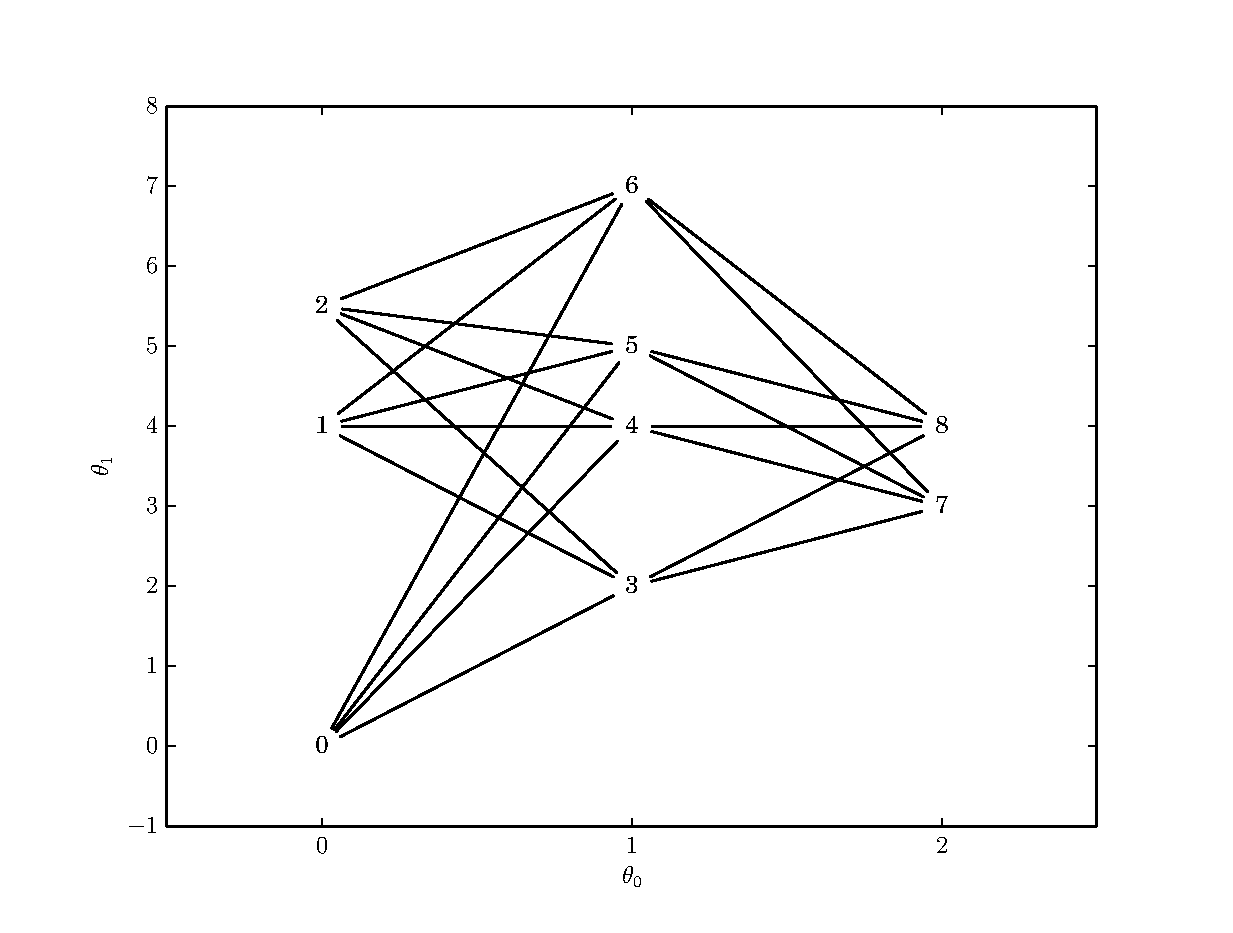
\includegraphics[width=\figwidthscale\textwidth]{plots/small_graph_ex.eps}
    \CaptionWithTitle{%
        \input{plots/small_graph_ex.txt}%
    }{\label{plot:simple_graph}}
\end{figure}

\begin{figure}[!t]
    \centering
    \includegraphics[width=\figwidthscale\textwidth]{plots/small_graph_ex_greedy_paths.eps}
    \CaptionWithTitle{%
        \input{plots/small_graph_ex_greedy_paths.txt}%
    }{\label{plot:simple_graph_greedy_paths}}
\end{figure}

\subsection{$L$ shortest paths via linear programming}

To find a set of paths minimizing the total cost, we instead search for total
solutions $\boldsymbol{x}$ that describe all paths in the graph. Assume for now
that we can guarantee that the entries of $\boldsymbol{x}$ will be either 0 or
1. To find a set of constraints for our search, we consider the structure of a
valid solution $\boldsymbol{x}^{\ast}$. To maintain that paths not overlap, a
valid solution's nodes are only allowed to have one edge entering ---
coming from a node in a previous frame --- and one edge leaving
--- going to a node in a successive frame. To translate this into a
constraint, consider the node $i$ and its possible $R_{i}$ successive connecting
nodes $j_{0} \dotsc j_{R_{i}-1}$. Define the vector\footnote{The superscript s
stands for ``successive''.}
\[
    a^{\text{s},i}_{i + Mj_{r}} = \begin{cases}
        1 & \forall j_{r} \in \left[ j_{0} \dotsc j_{R_{i}-1} \right] \\
        0 & \text{otherwise}
    \end{cases}
\]
As all the entries of $\boldsymbol{x}$ are either 0 or 1, we have
\[
    0 \leq \left\langle \boldsymbol{a}^{\text{s},i}, \boldsymbol{x} \right\rangle \leq 1
\]
so we can make this a constraint to ensure that a node has at most one path
leaving. Similarly, if we consider the node $j$ and its possible $R_{j}$ previous connecting
nodes $i_{0} \dotsc i_{R_{j}-1}$, the vector\footnote{The superscript p
stands for ``previous''.}
\[
    a^{\text{p},j}_{i_{r} + Mj} \begin{cases}
        1 & \forall i_{r} \in \left[ i_{0} \dotsc i_{R_{j}-1} \right] \\
        0 & \text{otherwise}
    \end{cases}
\]
constrains that node $j$ have only one path entering through the constraint
\[
    0 \leq \left\langle \boldsymbol{a}^{\text{p},j} , \boldsymbol{x} \right\rangle \leq 1
\]
A node on a path will also have an edge entering and an edge leaving. To
translate this into a constraint, we define a vector that counts the number of
edges entering a node and subtracts then the number of edges leaving a node. The
result should always be 0 for an equal number of edges entering and exiting a
node. If $r$ is the index of the node considered, the vector is simply
\footnote{The superscript b stands for ``balanced''.}
\[
    \boldsymbol{a}^{\text{b},r} = \boldsymbol{a}^{\text{p},r} -
    \boldsymbol{a}^{\text{s},r}
\]
and the constraint
\[
    \left\langle \boldsymbol{a}^{\text{b},r}, \boldsymbol{x} \right\rangle = 0
\]
Finally we want to constrain that there be only $L$ paths. We do this by
noticing that if this is true, there will be $L$ edges between frames $h$ and
$h+1$. We constrain the number of paths going from edges
$\Gamma_{h}$ in frame $h$ to $\Gamma_{h+1}$ by forming the vector
\footnote{The superscript c stands for ``connections''.}
\[
    \boldsymbol{a}^{\text{c},h} = \sum_{j \in \Gamma_{h}}
    \boldsymbol{a}^{\text{s},j}
\]
and asserting the constraint
\[
    \left\langle \boldsymbol{a}^{\text{c},h} , \boldsymbol{x} \right\rangle = L
\]
The length of $\boldsymbol{x}$ is $M^{2}$ so the total size of all the
constraints is not insignificant, but most entries in the constraint vectors will
be 0 and therefore the resulting constraint matrices very sparse, so sparse
linear algebra routines can be used in computations. Furthermore, the
$\boldsymbol{a}^{b}$ and $\boldsymbol{a}^{c}$ constraints are derived from
$\boldsymbol{a}^{p}$ and $\boldsymbol{a}^{s}$, so only the latter need to be
stored.

\begin{figure}[!t]
    \centering
    \includegraphics[width=\figwidthscale\textwidth]{plots/small_graph_ex_lp_paths.eps}
    \CaptionWithTitle{%
        \input{plots/small_graph_ex_lp_paths.txt}%
    }{\label{plot:simple_graph_lp_paths}}
\end{figure}

The complete \textit{linear program (LP)} solving the $L$ shortest paths problem is then
\[
    \min_{\boldsymbol{x}} \left\langle \boldsymbol{c}, \boldsymbol{x} \right\rangle
\]
subject to
\[
    \boldsymbol{0} \leq
    \begin{bmatrix}
        \boldsymbol{A}_{\text{s}} \\
        \boldsymbol{A}_{\text{p}}
    \end{bmatrix} \boldsymbol{x}
    \leq \boldsymbol{1}
\]
\[
    \begin{bmatrix}
        \boldsymbol{A}_{\text{b}} \\
        \boldsymbol{A}_{\text{c}}
    \end{bmatrix}
    \boldsymbol{x}
    =
    \begin{bmatrix}
        \boldsymbol{0} \\
        L\boldsymbol{1}
    \end{bmatrix}
\]
\[
    \boldsymbol{0} \leq \boldsymbol{x} \leq \boldsymbol{1}
\]
where $\boldsymbol{A}_{\text{s}}$ is the matrix with
$\boldsymbol{a}^{\text{s},m}$ as its rows for $m \in [0 \dotsc M-1]$ and
$\boldsymbol{A}_{\text{p}}$ is the matrix with $\boldsymbol{a}^{\text{p},m}$ as
its rows, etc.

The solution of the two best paths using the LP formulation
is shown in Figure~\ref{plot:simple_graph_lp_paths} and a comparison of the
total costs is shown in Table~\ref{tab:greedy_lp_cost_compare}

\begin{table}[!b]
    \caption{\label{tab:greedy_lp_cost_compare} Comparison of total costs in
    Figure~\ref{plot:simple_graph_lp_paths}}
    \begin{center}
        \begin{tabular}{c c}
            Greedy & LP \\
            \hline
            \input{plots/small_graph_ex_greedy_cost.txt} &
            \input{plots/small_graph_ex_lp_cost.txt} \\
        \end{tabular}
    \end{center}
\end{table}

The LP formulation is inspired by a multiple object tracking algorithm for video
\cite{jiang2007linear}. A proof that the solution $\boldsymbol{x}^{\ast}$ will
have entries equal to either $0$ or $1$ can be found in
\cite[p.~167]{parker1988discrete}. The theoretical computational complexity of
the linear program is polynomial in the number of variables, see
\cite{karmarkar1984new} for a proof and the demonstration of a fast algorithm
for finding its solution. In practice, to extract paths from the solution, we do
not test equality with $0$ or $1$ but rather test if the solution vector's
values are greater than some threshold. This may mean that suboptimal solutions
may still be close enough. The tolerance of the solutions to suboptimality
should be investigated, as if they are tolerant, fewer iterations of a
barrier-based algorithm would be required to solve the problem. More information
on linear programming and optimization in general can be found in
\cite{boyd2004convex}.

\subsection{Complexity}

The LP formulation of the $L$-best paths problem gives results equivalent to the
solution to the $L$-best paths problem proposed in \cite{wolf1989finding}. The
complexity of our algorithm is different.  Assuming we
use the algorithm in \cite{karmarkar1984new} to solve the LP, our program has a
complexity of $O(M^{7}B^{2})$ where $M$ is the number of nodes (parameter sets)
and $B$ is the number of bits used to represent each number in the input. The
complexity of the algorithm by Wolf in \cite{wolf1989finding} is equivalent to
the Viterbi algorithm for finding the single best path through a trellis whose
$h$th frame has $\binom{N_{h}}{L}\binom{N_{h+1}}{L}L!$ connections where $N_{h}$
and $N_{h+1}$ are the number of nodes in two consecutive frames of the original
lattice. Therefore, assuming a constant number $N$ of nodes in each frame, its
complexity is $O((\binom{N}{L}^{2}L!)^{2}T)$. If there are few nodes in each
frame and a small number of paths are searched, Wolf's formulation is superior
as its complexity increases linearly with the number of frames in the lattice.
On the other hand, if each frame has a large number of nodes or many paths are
searched, the LP formulation is superior.  Informally we have found this to
agree with reality --- both algorithms were tried when producing the figures in
Section~\ref{sec:mq_lp_compare_chirp}.  Indeed the Wolf formulation took
prohibitively long to compute when many paths were desired, as did the LP when
many frames were considered.

It should be noted that in the special case that only 1 shortest path is
searched an algorithm exists that requires on the order of $N^{2}T$ calculations
\cite{rabiner1989tutorial} where $N$ is the number of nodes in each frame and
$T$ is the number of frames (assuming the same number of nodes in each frame):
this algorithm is known as the Viterbi algorithm \cite{forney1973viterbi}.

\section{Partial paths on an example signal\label{sec:mq_lp_compare_chirp}}

We compare the greedy and LP based methods for peak matching on a synthetic
signal. The signal is composed of $K=6$ chirps of constant amplitude, the $k$th
chirp $s$ at sample $n$ described by the equation
\[
    s_{k}(n) = \exp(j(\phi_{k} + \omega_{k}n +
    \frac{1}{2} \psi_{k} n^{2}))
\]
The parameters for the 6 chirps are presented in
Table~\ref{tab:ptrackexamplechirpparams}.

\begin{table}[!b]
    \caption{Parameters of $k$th chirp. $f_{0}$ and $f_{1}$ are the initial and
    final frequency of the chirp in Hz. \label{tab:ptrackexamplechirpparams}}
    \begin{center}
        \begin{tabular}{l c c c c c}
            $k$ & $\phi_{k}$ & $\omega_{k}$ & $\psi_{k}$ & $f_{0}$ & $f_{1}$ \\
            \hline
            \input{plots/mq_lp_compare_chirp_params.txt}
        \end{tabular}
    \end{center}
\end{table}

Two 1 second long signals are synthesized at a sampling rate of 16000 Hz, the
first with chirps 0--2, the second with chirps 3--5. We add
Gaussian distributed white noise at several SNRs to evaluate the technique in the
presence of noise.

\begin{figure}[!t]
    %\centering
    \centering
    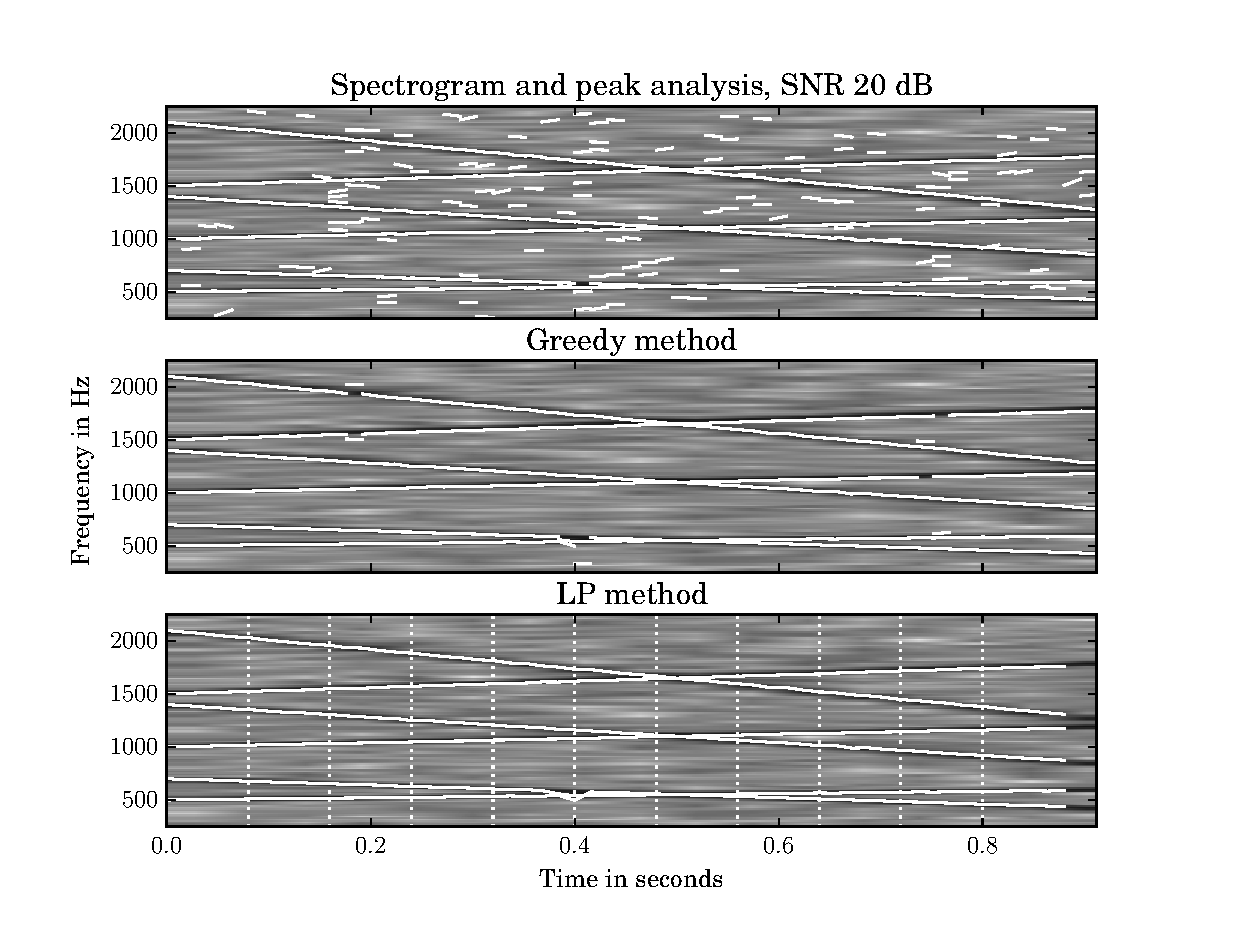
\includegraphics[width=\figwidthscale\textwidth]{plots/mq_lp_compare_chirp_20.eps}
    \CaptionWithTitle{%
        \input{plots/mq_lp_compare_chirp_20.txt}%
    }{ Line-segments representing the frequency and frequency-slope at local
        spectrogram maxima. In the bottom two plots the line segments not deemed
        by the respective algorithms as belonging to a partial path are
        discarded, revealing the estimated partial trajectories. See
        Table~\ref{tab:ptrackexamplechirpparams} for the chirp parameters.
    \label{plot:mq_lp_compare_chirp_20}}
\end{figure}
\begin{figure}[!t]
    %\centering
    \centering
    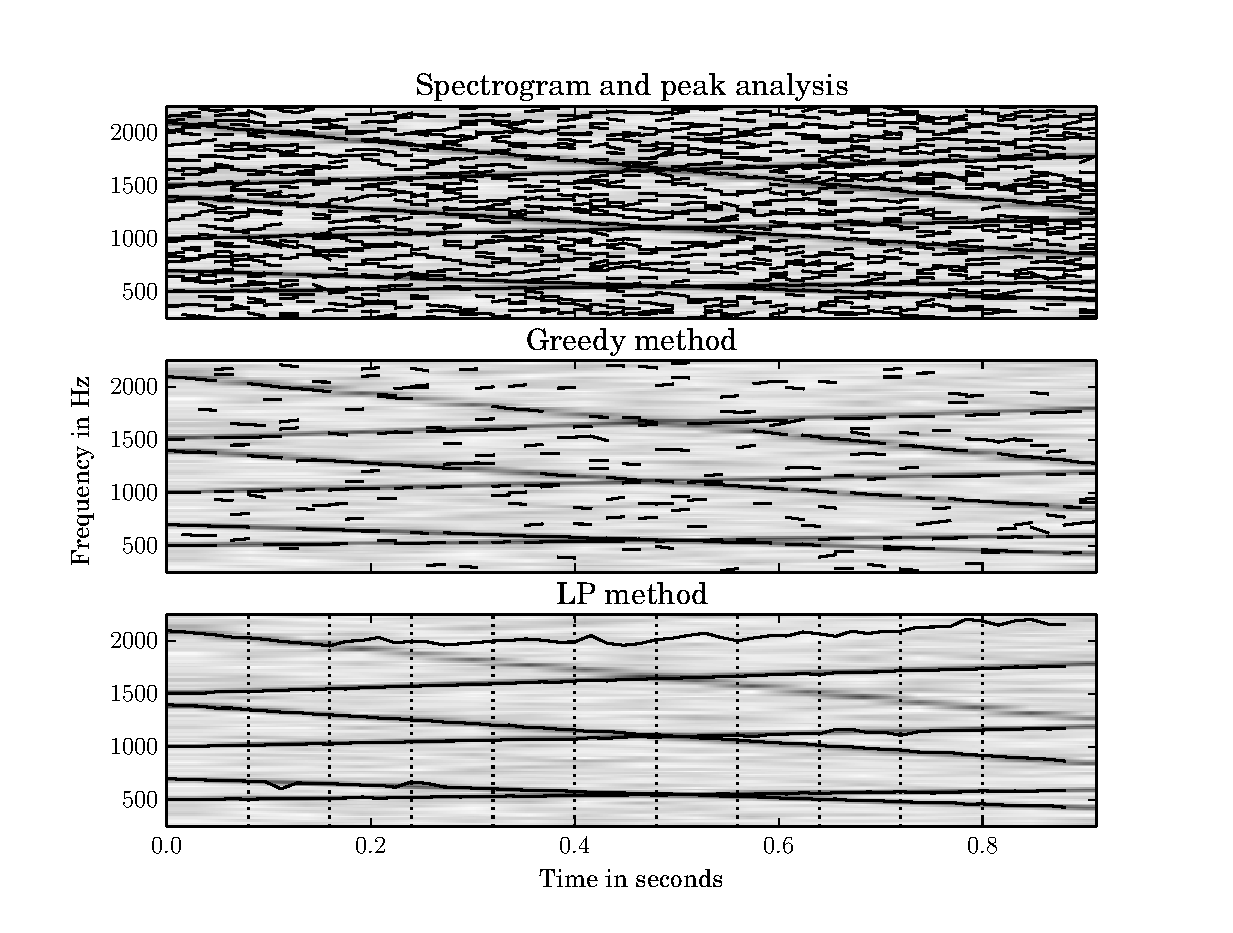
\includegraphics[width=\figwidthscale\textwidth]{plots/mq_lp_compare_chirp_15.eps}
    \CaptionWithTitle{%
        \input{plots/mq_lp_compare_chirp_15.txt}%
    }{ Line-segments representing the frequency and frequency-slope at local
        spectrogram maxima. In the bottom two plots the line segments not deemed
        by the respective algorithms as belonging to a partial path are
        discarded, revealing the estimated partial trajectories. See
        Table~\ref{tab:ptrackexamplechirpparams} for the chirp parameters.
    \label{plot:mq_lp_compare_chirp_15}}
\end{figure}
\begin{figure}[!t]
    %\centering
    \centering
    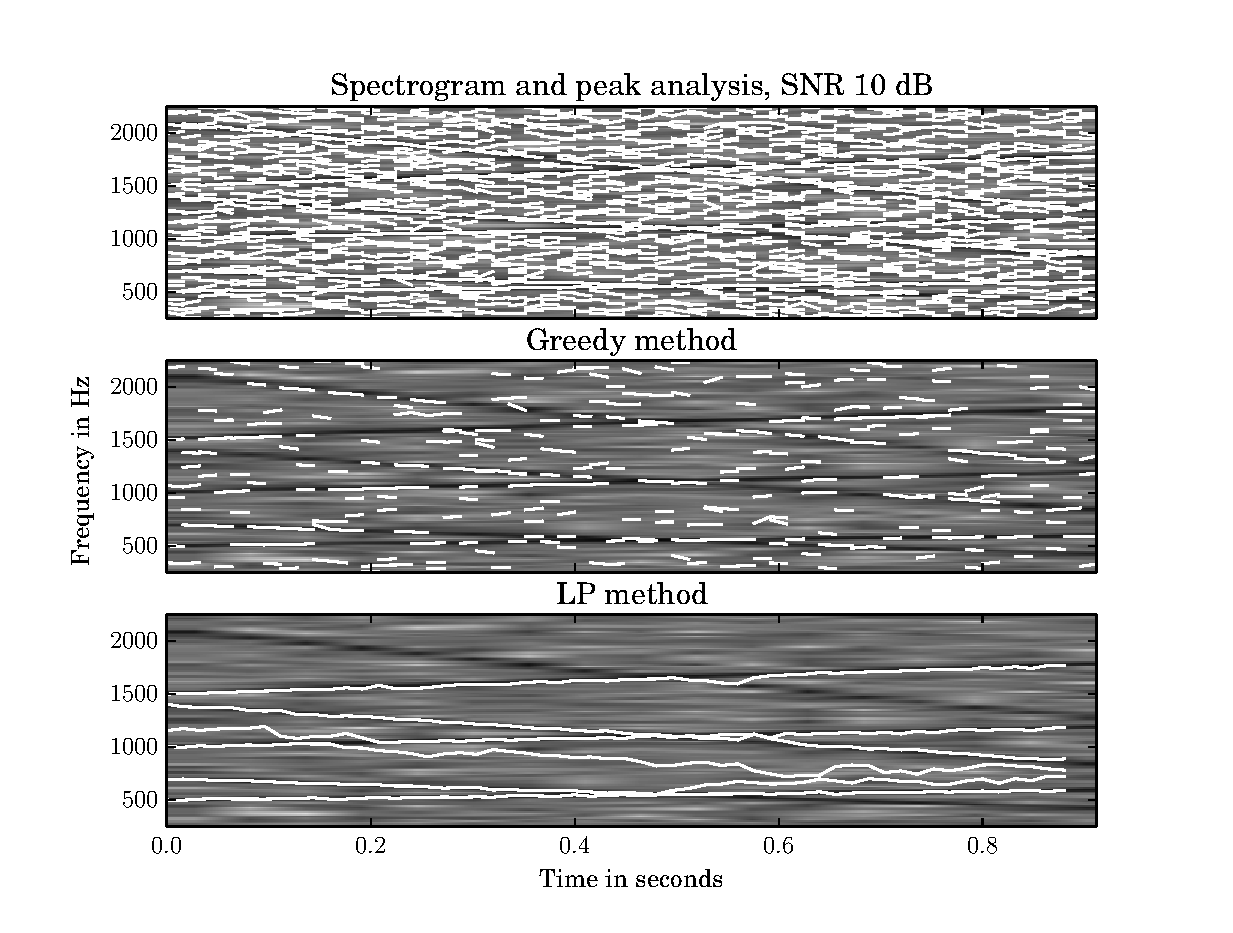
\includegraphics[width=\figwidthscale\textwidth]{plots/mq_lp_compare_chirp_10.eps}
    \CaptionWithTitle{%
        \input{plots/mq_lp_compare_chirp_10.txt}%
    }{ Line-segments representing the frequency and frequency-slope at local
        spectrogram maxima. In the bottom two plots the line segments not deemed
        by the respective algorithms as belonging to a partial path are
        discarded, revealing the estimated partial trajectories. See
        Table~\ref{tab:ptrackexamplechirpparams} for the chirp parameters.
    \label{plot:mq_lp_compare_chirp_10}}
\end{figure}

A spectrogram of each signal is computed with an analysis window length of 1024
samples and a hop-size $H$ of 256 samples. Local maxima are searched in 150 Hz
wide bands spaced 75 Hz apart. A local maximum is only accepted if its amplitude
is greater than -20 dB. At each local maximum the DDM is used to estimate the
local chirp parameters, the $i$th set of parameters in frame $h$ denoted
$\theta_{i}^{h} = \left\{ \phi_{i}^{h} , \omega_{i}^{h} , \psi_{i}^{h}
\right\}$. The results of the analyses of both signals are lumped together and
it is on this lumped data that we perform partial tracking.

We search for partial tracks using both the greedy and LP strategies. Both
algorithms use the distance metric $\mathcal{D}_{\text{pr.}}$ between two parameters sets:
\[
    \mathcal{D}_{\text{pr.}} \left( \theta_{i}^{h},
    \theta_{j}^{h+1} \right) = \left( \omega_{i}^{h} +
    \psi_{i}^{h} H - \omega_{j}^{h+1} \right)
\]
which is the error in predicting $j$th frequency in frame $h+1$ from the $i$th
parameters in frame $h$. For the greedy method, the search for partial paths is
restricted to one frame ahead like in \cite{mcaulay1986speech}. For the LP
method, to keep the computation time reasonable, we search over 6 frames for 6
best paths\footnote{The number of paths does not affect the computation time.}.
To maintain connected paths, the search on the next frames uses the end nodes of
the last search as starting points. For both methods, the search is restricted
to nodes between frequencies 250 to 2250 Hz.

Figures~\ref{plot:mq_lp_compare_chirp_20},~\ref{plot:mq_lp_compare_chirp_15},%
~and~\ref{plot:mq_lp_compare_chirp_10}
show discovered partial trajectories for signals with a SNR of 20, 15, and 10
dB,
respectively. It is seen that while the greedy method begins to perform poorly
at a SNR of 15dB, the LP method still gives plausible partial trajectories for
SNRs of 10 and 15 dB. At lower SNRs, the LP formulation gives
some paths that do not correspond to an underlying partial. These could be filtered
out by examining the cost of these paths and comparing them to the costs of the
others. Those that deviate from a mean cost more than a certain amount should be
rejected. This is the strategy used in Chapter~\ref{chap:decaysep} and
illustrated in Figure~\ref{plot:acgtra3xylofs4costlengththresh}. In any case,
the lower SNRs are relatively challenging for any partial tracking technique.

But why did the LP discover a path not present in the underlying signal? This is
due to the cost function, which finds a path with minimum prediction error in
using the frequency and frequency slope coefficients of one node to predict
another node's frequency coefficient. When there are many nodes in the original
analysis it is not surprising that some unexpected path exists.  An attribute of
these erroneous paths is that they are not smooth. To deter the algorithm from
finding such paths, regularization could be used like in
Section~\ref{sec:mqfmfromphase} that minimizes the integral of the squared
estimate of the path's second derivative. More on regularization in optimization
can be found in \cite[ch.~6.3]{boyd2004convex}.

\section{Conclusion}

In this chapter we reformulated the classical greedy algorithm of McAulay and
Quatieri and showed that it can be seen as a greedy algorithm for finding the $L$
shortest paths in a lattice. An algorithm was then proposed minimizing the sum
of the $L$ paths, using a linear programming approach. It was shown on synthetic
signals that the new approach finds plausible paths in lattices with a
large number of spurious nodes.

There are problems with the proposed approach. As discussed in
\ref{sec:lppathsearch}, ``jagged'' paths should be removed using regularization.
There are also situations where it is undesirable to have paths extend
throughout the entire lattice. Acoustic signals produced by striking media, such
as strings or bars, exhibit a spectrum where the upper partials decay more
quickly than the lower ones (e.g., see Figure~\ref{plot:acgtra3specgram}) --- it
would be desirable in these situations to have shorter paths for the upper
partials, those decaying more quickly. This could be addressed as in
\cite{depalle1993tracking} where the signal is divided into overlapping sequences of
frames and partial paths are connected between sequences.

The proposed algorithm, while faster than algorithms based on the Viterbi
algorithm, is still not fast. Assuming the same cost function
$\mathcal{D}_{\text{pr.}}$ as in Section~\ref{sec:mq_lp_compare_chirp} it would
be more efficient to consider narrow bands over which to search for paths when
analysing signals with little frequency modulation. However, as we will see in
Chapter~\ref{chap:amfmsep}, with different cost functions, the algorithm is
useful for solving general $L$ shortest paths problems outside of partial
tracking. 

% Problems:
% We assume paths spanning entire analysis are optimal

% Could also try and maximize smoothness of trajectories by adding second order
% differences as a cost.

%As a further test, we give the algorithms a hint by
%removing all spurious data-points from the first frame. We can see in
%Figures~\ref{plot:mq_lp_compare_chirp_hint15}~and~\ref{plot:mq_lp_compare_chirp_hint20}
%that this improves the results for the LP method.


\chapter{The extended phase and amplitude model\label{chap:exphsmodel}}

In Chapter~\ref{chap:partialtracking} techniques were presented for discovering
partials in a signal. Each partial is a set of analysis points indexed by time.
The information at each analysis point can be used to synthesize a portion of
the partial and these are combined to give a signal representing a partial.
The various techniques to synthesize these pieces of the signal discussed here
differ in the orders used for analysis and those for synthesis. The first
technique presented simply synthesizes signals of short duration using the
estimated parameters and blends these segments together. We recognize that
having multiple estimations of parameters at discrete times within the partial
duration allow us to postulate, via interpolation, functions describing the
partial of higher-order than those whose parameters were estimated during
analysis. It is shown that this strategy is not always to our advantage ---
interpolants of higher-order than the underlying function can suffer from errors
due to over-fitting. In the case of functions that are always better
approximated by higher-order polynomials, we will see that there is an advantage
to using high order interpolation. These cases are illustrated through the
analysis and synthesis of synthetic signals.

\section{Partial synthesis \label{sec:partialsynthesis}}

A popular technique for synthesizing partials from a set of analysis points is
the \textit{overlap-and-add} procedure \cite{portnoff1976implementation},
\cite{moore1990elements}. We assume that in the neighbourhood of $\tau_{r}$ the
partial's signal is approximately described by the function $x(n) \approx
f_{\tau_{r}}(n-\tau_{r})$. To synthesize an approximation of $x$ we sum windowed
$f_{\tau_{r}}$ at multiple locations, windowed by a function $w$ with finite
support so the resulting signal has finite energy and the piecewise assumption
is maintained. For simplicity we assume the $\tau_{r}$ are equally spaced by $H$
samples, and $\tau_{0}=0$, so we have $\tau_{r} = rH$. The length of the window
function $w$ is $M = VH + 1$ samples, with $V,H \in \mathbb{N}%
$\footnote{%
    $M$ is always odd so one may wonder how the Fast Fourier Transform can be
    used to invert $F_{\tau_{r}}$, the frequency-domain representation of
    $f_{\tau_{r}}$.  Recall that the DTFT can be interpreted as the coefficients
    of a Fourier series that give the periodic version of the analysed signal.
    Also recall that we use window functions that are real and even. In practice
    the edges of the window are often equal to zero so that the length of the
    non-zero part is equal to the length of the DTFT $N$. In the case they are
    not, simply ensuring that values in the window indexed by integer multiples
    of $N$ are 0, and that the value at the centre of the window is 1 will ensure proper
    synthesis \cite[p.~244]{portnoff1976implementation}. In that case, the values
    outside of the part of the window presented to the DTFT are folded into this
    region using the window indices modulo-$N$. See
    \cite{portnoff1976implementation} and \cite{moore1990elements} for more details on this
    procedure.%
}.
The approximate signal at sample $n$ is then
\[
    \tilde{x}(n) = \sum_{l=L_{-}}^{L^{+}} w(n-lH) f_{\tau_l}(n-\tau_l)
\]
where
\[
    L_{-} = \left\lceil \frac{n}{H} \right\rceil - V
\]
and
\[
    L_{+} = \left\lfloor \frac{n}{H} \right\rfloor + V
\]
This method has some drawbacks. Usually the function $f$ is an approximation
$\tilde{f}$ of the true underlying function. In the case of partial tracking,
often partials that are too short are discarded or missed. At amplitude
transients, these short partials are important for reproducing sharp attacks
that are shorter than the window length. If these partials are missing, the
resulting signal takes on a transient similar to the window shape. This could be
overcome by choosing a window with a shape similar to the overall amplitude
envelope in the attack region when resynthesizing an attack transient.

Another drawback is that no attempt is made to interpolate between the functions
estimated at $\tau_{r}$ and $\tau_{r+1}$ using the model that the underlying
sinusoids are non-stationary\footnote{%
    This is one of the causes of ``pre-echo'' when
    time-stretching using the STFT \cite{roebel2003transient}.%
}
From Equation~\ref{eq:ddmsyseq} we know we can estimate a polynomial of
arbitrary order for the argument of the complex exponential. We will see that
using this additional information can give us an interpolating function closer
to the underlying model.

\section{The interpolating analysis-synthesis system}

In the following, we investigate the synthesis quality of three interpolating
analysis-synthesis systems. The qualifier ``interpolating'' is used because each
system takes the multiple sets of estimated parameters of a smaller order model
and interpolates them with a higher-order model, which is then used for
synthesis. This is necessary because we only have values every $H$ samples from
the analysis step but require a value for every sample value in the output. The
systems will be denoted $\mathscr{S}_{p,q}$ where $p$ is the order of the
analysis system and $q$ the order of the synthesis system, e.g., a linear
analysis system has $p=1$, etc.

\section{$\mathscr{S}_{1,3}$: the McAulay-Quatieri method}

\subsection{Analysis: linear phase and constant amplitude%
\label{sec:S13analysis}}

For the McAulay-Quatieri method, the analysis model is a sinusoid of constant frequency
and amplitude
(linear phase and constant log-amplitude) in each analysis frame. To estimate the frequency of this
sinusoid we find the bin with the most energy and find a refined estimate of the
frequency as the maximum of a quadratic interpolating polynomial fit to this bin
and its two neighbouring bins. This is a procedure documented in
\cite[p.~45]{serra1989system}. The interpolation is best performed in the
log-spectrum and on a spectrum produced using a window, such as a zero-padded
Hann window, giving a wide enough main-lobe so that the three points lie on this
lobe and not on side-lobes. A refined estimate of the amplitude of the sinusoid
is obtained with this procedure as well.

In the original paper by McAulay and Quatieri, they do not use this technique
but, as they show an example analysis of a speech signal, instead adjust the
analysis window to be a multiple of the period of the glottal pulse. The bins of
the DTFT used in the analysis will be integer multiples of the frequency given
as the reciprocal of this period. Under the model of the speech signal as
harmonically related sinusoids, the best estimate for the frequency is the bin
of a local maximum, its amplitude the modulus of the spectrum at this maximum, and
the phase the argument.

In our system, we use a fixed window size. To estimate the initial phase then we use
Equation~\ref{eq:ddmestc0} with
\[
    \gamma_{\text{MQ}}(n)=\exp(2\pi\frac{k^{\ast}}{M}n)
\]
where $k^{\ast}$ is the bin we have determined to correspond to the frequency of
the sinusoid. The initial phase is then $\Im \left\{ c_{0} \right\}$.

\subsection{Synthesis: cubic phase and linear log-amplitude \label{sec:S13synthesis}}

\subsubsection{The phase part}

Given two local maxima of the
DTSTFT $X(\tau_0,\omega_0)$ and $X(\tau_1,\omega_1)$, where $H = \tau_1 -
\tau_0$ we can conjecture a cubic
polynomial phase function for the imaginary part of the phase argument

\[
    \tilde{\phi}(n) = \Im\left\{c_3\right\} (n-\tau_0)^3 + \Im\left\{c_2\right\} (n-\tau_0)^2 + \Im\left\{c_1\right\} (n-\tau_0) + \Im\left\{c_0\right\}
\]

By noting that we have 2 measurements of the phase and frequency,
$\angle\{X(\tau_0,\omega_0)\}$ and $\angle\{X(\tau_1,\omega_1)\}$, and the frequency
is the derivative of the phase, we can solve for the coefficients of the
polynomial phase function using the following linear system of equations,
assuming the DTSTFT was computed using a real and even window
\[
    \begin{pmatrix}
        0   & 0     & 0 & 1 \\
        H^3 & H^2   & H & 1 \\
        0   & 0     & 1 & 0 \\
        3 H^2 & 2 H & 1 & 0
    \end{pmatrix}
    \begin{pmatrix}
        \Im\{c_3\} \\
        \Im\{c_2\} \\
        \Im\{c_1\} \\
        \Im\{c_0\}
    \end{pmatrix}
    =
    \begin{pmatrix}
        \angle\{X(\tau_0,\omega_0)\} \\
        \angle\{X(\tau_1,\omega_1)\} + 2 \pi M \\
        \omega_0 \\
        \omega_1        
    \end{pmatrix}
\]
We choose $M$ so that
\begin{equation}
    \label{eq:minfmmq}
    \int_{0}^{H}(\frac{d^{2}\tilde{\phi}}{dt^2}(t))^{2}dt
\end{equation}
is minimized in order to have a smooth evolution of phase in the interpolated
region. $M$ is necessary because some integer number of periods of a sinusoid
will have passed from times $\tau_{0}$ to $\tau_{1}$. Informally we choose $M$
so that a polynomial describing the phase evolution between these two times
takes a direct route, which is a plausible criterion because a signal with more
radical phase variation would unlikely exhibit a spectrum that could be well
described by two points in the time-frequency plane, i.e., the signal
would exhibit a large bandwidth. See \cite[p.~751]{mcaulay1986speech} for
further clarification.

\subsubsection{The amplitude part}

As only two measurements of the amplitude of the sinusoid are available,
$|X(\tau_0,\omega_0)|$ and $|X(\tau_1,\omega_1)|$, the coefficients
$c_3$ and $c_2$ are purely imaginary and the real parts of $c_1$ and $c_0$ are
determined as
\[
    \begin{pmatrix}
        0 & 1 \\
        H & 1
    \end{pmatrix}
    \begin{pmatrix}
        \Re\{c_1\} \\
        \Re\{c_0\}
    \end{pmatrix}
    =
    \begin{pmatrix}
        \log(|X(\tau_0,\omega_0)|) \\
        \log(|X(\tau_1,\omega_1)|)
    \end{pmatrix}
\]

\section{$\mathscr{S}_{2,3}$ and $\mathscr{S}_{2,5}$: the DDM-based methods}

Here we extend the $\mathscr{S}_{1,3}$ model of McAulay-Quatieri to account for
the additional parameters estimated via the DDM. For the $\mathscr{S}_{2,3}$
model, we must introduce additional constraints into the system as we have more
estimated parameters than are available in the synthesis model. It would be
possible to solve this system via least-squares, but the proposed constraints
simplify analytically the expression maximizing the smoothness of the phase and
log-amplitude
functions, and give satisfactory results. For the $\mathscr{S}_{2,5}$ model the
derivation is straightforward as in the $\mathscr{S}_{1,3}$ case --- there are
the same number of estimated parameters as there are parameters in the model.

\subsection{Analysis: quadratic phase and log-amplitude \label{sec:s235analysis}}

The DDM is used on segments of the signal to estimate the parameters of sinusoid
with a complex quadratic polynomial argument. This sinusoid has the form
\begin{equation}
    \label{eq:quadraticphasepoly}
    x_{a}(n) = \exp \left(a_2 n^{2} + a_1 n + a_0 \right)
\end{equation}
with $a_{i} \in \mathbb{C}$.

We can estimate the coefficients of Equation~\ref{eq:quadraticphasepoly} using
the DDM. We write Equation~\ref{eq:ddmsyseq} in matrix form with $Q=2$
\[
    \begin{pmatrix}
        \left\langle \mathcal{T}^{0} x , \overline{\psi}_{1} \right\rangle &
        2\left\langle \mathcal{T}^{1} x , \overline{\psi}_{1} \right\rangle \\
        \vdots & \vdots \\
        \left\langle \mathcal{T}^{0} x , \overline{\psi}_{R} \right\rangle & 
        2\left\langle \mathcal{T}^{1} x , \overline{\psi}_{R} \right\rangle
    \end{pmatrix}
    \begin{pmatrix}
        a_{1} \\
        a_{2}
    \end{pmatrix}
    =
    \begin{pmatrix}
        -\left\langle  x , \frac{d\overline{\psi}_{1}}{dn} \right\rangle \\
        \vdots \\
        -\left\langle  x , \frac{d\overline{\psi}_{R}}{dn} \right\rangle
    \end{pmatrix}
\]

From this we recognize we need to define three functions
\[
    \left\langle \mathcal{T}^{0} x , \overline{\psi}_{k} \right\rangle 
    =
    \sum_{m=0}^{M-1} w(m) x(m + \tau) \exp(-j 2 \pi \frac{k m}{M})
\]
\[
    \left\langle \mathcal{T}^{1} x , \overline{\psi}_{k} \right\rangle
    =
    \sum_{m=0}^{M-1} m w(m) x(m + \tau) \exp(-j 2 \pi \frac{k m}{M})
\]
\[
    \left\langle  x , \frac{d\overline{\psi}_{k}}{dn} \right\rangle
    =
    -j 2 \pi \frac{k}{M} X_{p_{1}} \left( \tau , k \right) + 
    \sum_{m=0}^{M-1} \frac{dw}{dn}(m) x(m + \tau) \exp(-j 2 \pi \frac{k m}{M})
\]
Where $M$ is the length of the window and $k$ is the frequency
``bin''\footnote{For tractability, the functions $X(\tau,k)$ are only evaluated at
    a finite number of frequencies, which are often called ``bins'' in the
signal processing literature.}. We also
only consider $x$ at the samples $m = [0, \dotsc, M-1]$ because we can always
shift the time reference to view an arbitrary contiguous segment of signal with
these indices.

We then find $k^{\ast}$ such that $X$ is maximum. If multiple components
are present in the signal and are sufficiently separated in frequency, we can
split the signal up into frequency bands and find local maxima. A technique for
doing so is described in \cite[p.~42]{serra1989system}. To have a system of
equations with a unique solution, we take the two adjacent bins $k-1$ and $k+1$
to have enough unique atoms for Equation~\ref{eq:ddmsyseq}. These bins should
only contain energy from the component whose parameters we are interested in
measuring --- this is true if the components are adequately separated in time
and frequency. We could choose only two bins to have a non-singular system, and
there are many possibilities for choosing different atoms
\cite[p.~4639]{betser2009sinusoidal}. We choose three from the same frame to
have improved estimation accuracy in situations where components are adequately
separated in frequency, while avoiding a more sophisticated local peak selection
procedure. Then $a_2$ and $a_1$ can be determined by solving the linear system
\[
    \begin{pmatrix}
        \left\langle \mathcal{T}^{0} x , \overline{\psi}_{k-1} \right\rangle &
        \left\langle \mathcal{T}^{1} x , \overline{\psi}_{k-1} \right\rangle \\
        \left\langle \mathcal{T}^{0} x , \overline{\psi}_{k} \right\rangle &
        \left\langle \mathcal{T}^{1} x , \overline{\psi}_{k} \right\rangle \\
        \left\langle \mathcal{T}^{0} x , \overline{\psi}_{k+1} \right\rangle & 
        \left\langle \mathcal{T}^{1} x , \overline{\psi}_{k+1} \right\rangle
    \end{pmatrix}
    \begin{pmatrix}
        a_{1} \\
        2a_{2}
    \end{pmatrix}
    =
    \begin{pmatrix}
        -\left\langle  x , \frac{d\overline{\psi}_{k-1}}{dn} \right\rangle \\
        -\left\langle  x , \frac{d\overline{\psi}_{k}}{dn} \right\rangle \\
        -\left\langle  x , \frac{d\overline{\psi}_{k+1}}{dn} \right\rangle
    \end{pmatrix}
\]
With $a_{1}$ and $a_{2}$ determined, we can use Equation~\ref{eq:ddmestc0} to
estimate $a_0$. We will write $a^{\tau}_{i}$ to refer to coefficient $i$
determined at time $\tau$.

\subsection{Synthesis: cubic order ($\mathscr{S}_{2,3}$)
\label{sec:s23synthesis}}

In this section we describe how to obtain a cubic phase and log-amplitude polynomial from
local estimations of the coefficients of a quadratic phase and log-amplitude polynomial.

\subsubsection{The phase part}

A complex sinusoid with cubic phase has the following form:
\begin{equation}
    \label{eq:cubicphasepoly}
    \beta(n) = \exp \left(j\left(b_3 n^{3} + b_2 n^{2} + b_1 n + b_0
        \right)\right)
\end{equation}
with $b_{i} \in \mathbb{R}$. This sinusoid has magnitude 1 everywhere, only its
phase is changing.

Once the $\boldsymbol{a}^{\tau}$ have been determined
at two times $\tau_{0}$ and $\tau_{1}$, with $H = \tau_{1} - \tau_{0}$, and these
times have between determined as connected (see
Chapter~\ref{chap:partialtracking}), we can write a system of equations
to determine an interpolating cubic phase polynomial. To avoid numerical
instabilities and for simplicity, we shift the time origin so that $\tau_{0} =
0$. This means $b_0 = \Im \left\{ a^{\tau_0}_{0} \right\}$. To reduce the size
of the system, we require that 
\[
    \frac{d \phi}{d n} \left(\frac{H}{2} \right)
    =
    \frac{1}{2}
    \left( \Im \left\{ a^{\tau_0}_{1} \right\} + \Im \left\{ a^{\tau_1}_{1}
    \right\} \right)
\]
and
\[
    \frac{d^{2} \phi}{d n^{2}} \left(\frac{H}{2}
    \right)
    =
    \frac{1}{2} \left( \Im \left\{ a^{\tau_0}_{2} \right\} + \Im \left\{
    a^{\tau_1}_{2} \right\} \right)
\]
i.e., the frequency and first-order frequency modulation in the middle of the
segment are the average of the two measured coefficients. Finally we require
that the change in phase from time $0$ to $H$ correspond to that what was
observed, but account for the cycles that were not observed by adding an integer
number of $2\pi$ radians. If $\phi(n)=j(b_3 n^{3} + b_2 n^{2} + b_1 n + b_0)$,
then
\[
    \phi \left( H \right)
    =
    \Im \left\{ a^{\tau_1}_{0} \right\} - \Im \left\{ a^{\tau_0}_{0} \right\}
    + 2 \pi U^{\ast}
\]
where $U^{\ast} \in \mathbb{Z}$ is determined to minimize
Equation~\ref{eq:minfmmq}, in this case:
\begin{equation}
    \label{eq:minfmcubic}
    \tilde{U} = \argmin_{U} \int_{0}^{H} \left(
    6 b_3 t + 2 b_2 \right)^{2} dt
\end{equation}
which is then rounded to the nearest integer to give $U^{\ast}$. To summarize we have
\[
    \begin{pmatrix}
        H^{3} & H^{2} & H \\
        \frac{3}{4}H^{2} & H & 1 \\
        3 H & 2 & 0
    \end{pmatrix}
    \begin{pmatrix}
        b_{3} \\
        b_{2} \\
        b_{1}
    \end{pmatrix}
    =
    \begin{pmatrix}
        \Im \left\{ a^{\tau_1}_{0} \right\} - \Im \left\{ a^{\tau_0}_{0} \right\}
            + 2 \pi U^{\ast} \\
        \frac{1}{2}
        \left( \Im \left\{ a^{\tau_0}_{1} \right\} + \Im \left\{ a^{\tau_1}_{1}
        \right\} \right) \\
        \frac{1}{2} \left( \Im \left\{ a^{\tau_0}_{2} \right\} + \Im \left\{
        a^{\tau_1}_{2} \right\} \right)
    \end{pmatrix}
\]
Solving for $b_1, \dotsc, b_3$, we have
\[
    \begin{pmatrix}
        b_{3} \\
        b_{2} \\
        b_{1}
    \end{pmatrix}
    =
    \begin{pmatrix}
        \frac{4}{H^3} \left( \Im \left\{ a^{\tau_1}_0 \right\}
            - \Im \left\{ a^{\tau_0}_0 \right\} + 2 \pi U^{\ast} \right)
        - \frac{2}{H^{2}} \left( \Im \left\{ a^{\tau_1}_1 \right\}
            + \Im \left\{ a^{\tau_0}_1 \right\} \right) \\
        \frac{-6}{H^2} \left( \Im \left\{ a^{\tau_1}_0 \right\}
            - \Im \left\{ a^{\tau_0}_0 \right\} + 2 \pi U^{\ast} \right)
        - \frac{3}{H} \left( \Im \left\{ a^{\tau_1}_1 \right\}
            + \Im \left\{ a^{\tau_0}_1 \right\} \right)
        + \frac{1}{4}  \left( \Im \left\{ a^{\tau_0}_{2} \right\} + \Im \left\{
            a^{\tau_1}_{2} \right\} \right) \\
        \frac{-H}{4}  \left( \Im \left\{ a^{\tau_0}_{2} \right\} + \Im \left\{
            a^{\tau_1}_{2} \right\} \right) 
        + \frac{3}{H} \left( \Im \left\{ a^{\tau_1}_0 \right\}
            - \Im \left\{ a^{\tau_0}_0 \right\} + 2 \pi U^{\ast} \right)
        -  \Im \left\{ a^{\tau_1}_1 \right\}
            - \Im \left\{ a^{\tau_0}_1 \right\}
    \end{pmatrix}
\]
and then $\tilde{U}$ is determined using Equation~\ref{eq:minfmcubic} to be
\[
    \tilde{U} = \frac{1}{4 \pi} \left[ H \left( \Im \left\{ a^{\tau_1}_1
            \right\} + \Im \left\{
        a^{\tau_0}_1 \right\} \right)
        -2 \left( \Im \left\{ a^{\tau_1}_0 \right\} - \Im \left\{
        a^{\tau_0}_0 \right\} \right) \right]
\]
and then rounded to obtain $U^{\ast}$.

\subsubsection{The amplitude part}

Solving for the cubic polynomial describing the local log-amplitude function
\[
    \mu(n) = \exp \left(d_3 n^{3} + d_2 n^{2} + d_1 n + d_0 \right)
\]
with $d_i \in \mathbb{R}$, is more straightforward analytically as it does not
require solving to maximize the smoothness of resulting polynomial. To require
continuity at the end-points of our polynomial, we require
\[
    \mu(0) = \Re \left\{ a^{\tau_0}_0 \right\}
\]
and
\[
    \mu(H) = \Re \left\{ a^{\tau_1}_0 \right\}
\]
The first constraint is satisfied simply by setting $d_0 = \Re \left\{
a^{\tau_0}_0 \right\}$. The second will be accounted for in a constrained
least-squares solution for the other coefficients. The other observations are
\[
    \frac{d \mu}{dn} (0) = \Re \left\{ a^{\tau_0}_1 \right\}
\]
\[
    \frac{d \mu}{dn} (H) = \Re \left\{ a^{\tau_1}_1 \right\}
\]
\[
    \frac{d^2 \mu}{dn^2} (0) = \Re \left\{ a^{\tau_0}_2 \right\}
\]
\[
    \frac{d^2 \mu}{dn^2} (H) = \Re \left\{ a^{\tau_1}_2 \right\}
\]
The constrained least-squares problem to be solved is then
\[
    \begin{pmatrix}
        0 & 0 & 1 \\
        3 H^2 & 2 H & 1 \\
        0 & 2 & 0 \\
        6 H & 2 & 0
    \end{pmatrix}
    \begin{pmatrix}
        d_3 \\
        d_2 \\
        d_1
    \end{pmatrix}
    =
    \begin{pmatrix}
        \Re \left\{ a^{\tau_0}_1 \right\} \\
        \Re \left\{ a^{\tau_1}_1 \right\} \\
        \Re \left\{ a^{\tau_0}_2 \right\} \\
        \Re \left\{ a^{\tau_1}_2 \right\}
    \end{pmatrix}
\]
subject to
\[
    \begin{pmatrix}
        H^3 & H^2 & H
    \end{pmatrix}
    \begin{pmatrix}
        d_3 \\
        d_2 \\
        d_1
    \end{pmatrix}
    =
    \begin{pmatrix}
        \Re \left\{ a^{\tau_1}_0 \right\}
    \end{pmatrix}
\]
This can be solved using numerical methods, in particular, using a specific
interpretation of weighted least-squares \cite[p.~266]{golub1996matrix}.

\subsection{Synthesis: quintic order ($\mathscr{S}_{2,5}$) \label{s25synthesis}}

\subsubsection{The phase part}

Solving for the coefficients of a quintic phase polynomial is done very
similarly to Section~\ref{sec:s23synthesis}. As we have the same number of
analysis and synthesis parameters, no constraints have to be
introduced to solve the system apart from the value $U$ that maximizes
smoothness of the phase function. The quintic phase polynomial is%
\footnote{Remember, this sinusoid has constant amplitude of 1 and
this function only describes its change of phase.}
\begin{equation}
    \label{eq:quinticphasepoly}
    \lambda(n) = \exp \left(j\left(u_5 n^{5} + u_4 n^{4} + u_3 n^{3} + u_2 n^{2}
    + u_1 n + u_0 \right)\right)
\end{equation}
with $u_i \in \mathbb{R}$. We have
\[
    \phi(0) = \Im \left\{ a^{\tau_0}_0 \right\}
\]
\[
    \frac{d \phi}{d n}(0) = \Im \left\{ a^{\tau_0}_1 \right\}
\]
\[
    \frac{d^{2} \phi}{d n^{2}}(0) = \Im \left\{ a^{\tau_0}_2 \right\}
\]
and solving for the remaining coefficients is done using the linear system of
equations:
\[
    \begin{pmatrix}
        H^5 & H^4 & H^3 \\
        5 H^4 & 4 H^3 & 3 H^2 \\
        20 H^3 & 12 H^2 & 6 H
    \end{pmatrix}
    \begin{pmatrix}
        u_5 \\
        u_4 \\
        u_3
    \end{pmatrix}
    =
    \begin{pmatrix}
        -\frac{ H^{2} }{2} \ImNe{ a^{\tau_0}_2 } - H \ImNe{ a^{\tau_0}_1 } +
            \ImNe{ a^{\tau_1}_0 } - \ImNe{ a^{\tau_1}_1 } + 2 \pi U^{\ast}\\
        -H \ImNe{ a^{\tau_0}_2 } + \ImNe{ a^{\tau_1}_1 } - \ImNe{ a^{\tau_0}_1 } \\
        \ImNe{ a^{\tau_1}_2 } - \ImNe{ a^{\tau_0}_2 }
    \end{pmatrix}
\]
The smoothness maximizing $\tilde{U}$ is found as
% M=np.round((20.*H*(w_i0+w_i1)+(H**2.)*(psi_i0-psi_i1)+40.*(phi_i0-phi_i1))/(80.*np.pi))
\[
    \tilde{U} = \frac{1}{80 \pi} \left[ 20 H ( \ImNe{ a^{\tau_0}_1 } + \ImNe{ a^{\tau_1}_1 } )
        + H^2 ( \ImNe{ a^{\tau_0}_2 } - \ImNe{ a^{\tau_1}_2 } )
        + 40 ( \ImNe{ a^{\tau_0}_0 } - \ImNe{ a^{\tau_1}_0 } ) \right]
\]
and then rounded to produce $U^{\ast}$ as above.

The quintic interpolating phase polynomial has been proposed in a previous paper
\cite{girin2003comparing} although they do not directly estimate the frequency
slope, choosing instead to derive it using the difference in frequency between
two analysis frames.

\subsubsection{The amplitude part}

Solving for the quintic log-amplitude polynomial
\begin{equation}
    \label{eq:quinticamppoly}
    \rho(n) = \exp \left(v_5 n^{5} + v_4 n^{4} + v_3 n^{3} + v_2 n^{2} + v_1 n + v_0 \right)
\end{equation}
with $v_i \in \mathbb{R}$, is as follows:
\[
    \mu(0) = \Re \left\{ a^{\tau_0}_0 \right\}
\]
\[
    \frac{d \mu}{d n}(0) = \Re \left\{ a^{\tau_0}_1 \right\}
\]
\[
    \frac{d^{2} \mu}{d n^{2}}(0) = \Re \left\{ a^{\tau_0}_2 \right\}
\]
and solving for the remaining coefficients is done using the linear system of
equations:
\[
    \begin{pmatrix}
        H^5 & H^4 & H^3 \\
        5 H^4 & 4 H^3 & 3 H^2 \\
        20 H^3 & 12 H^2 & 6 H
    \end{pmatrix}
    \begin{pmatrix}
        v_5 \\
        v_4 \\
        v_3
    \end{pmatrix}
    =
    \begin{pmatrix}
        -\frac{ H^{2} }{2} \ReNe{ a^{\tau_0}_2 } - H \ReNe{ a^{\tau_0}_1 } +
            \ReNe{ a^{\tau_1}_0 } - \ReNe{ a^{\tau_1}_1 } \\
        -H \ReNe{ a^{\tau_0}_2 } + \ReNe{ a^{\tau_1}_1 } - \ReNe{ a^{\tau_0}_1 } \\
        \ReNe{ a^{\tau_1}_2 } - \ReNe{ a^{\tau_0}_2 }
    \end{pmatrix}
\]

\section{Evaluation}

We compared the quality of an analysis-synthesis system using the original
$\mathscr{S}_{1,3}$ method, $\mathscr{S}_{2,3}$ method, and the
$\mathscr{S}_{2,5}$. Frequency- and amplitude-modulated sinusoids were
synthesized and then analysed frame-by-frame using the DDM to estimate their
initial phase (amplitude), frequency (amplitude slope), and frequency-modulation
(amplitude-modulation). Afterwards, the signals were resynthesized using the
estimated parameters and compared to the original.  We are interested in seeing
in what cases higher-order phase and log-amplitude polynomials will improve the accuracy of
synthesis.

\subsection{Evaluation on a sinusoid of cubic phase and quartic log-amplitude \label{sec:evalcubicphase}}
\begin{table}
    \caption{\label{tab:cubicsinphparams}}
    \begin{center}
        \begin{tabular}{l|c c c}
            Time (seconds) & 0 & 0.25 & 0.5 \\
            Frequency (Hz) & 100 & 200 & 100
        \end{tabular}
    \end{center}
\end{table}
\begin{table}
    \caption{\label{tab:quarticsinampparams}}
    \begin{center}
        \begin{tabular}{l|c c c c}
            Time (seconds) & 0 & 0.1 & 0.3 & 0.5 \\
            Amplitude (dB) & -10 & 0 & 0 & -10
        \end{tabular}
    \end{center}
\end{table}

% Plots of this section produced with
% mq_cubic_test_less_fm_{1..3}.py
% compare_mq_interp_funcs_1.py
\begin{figure}[!t]
    \centering
    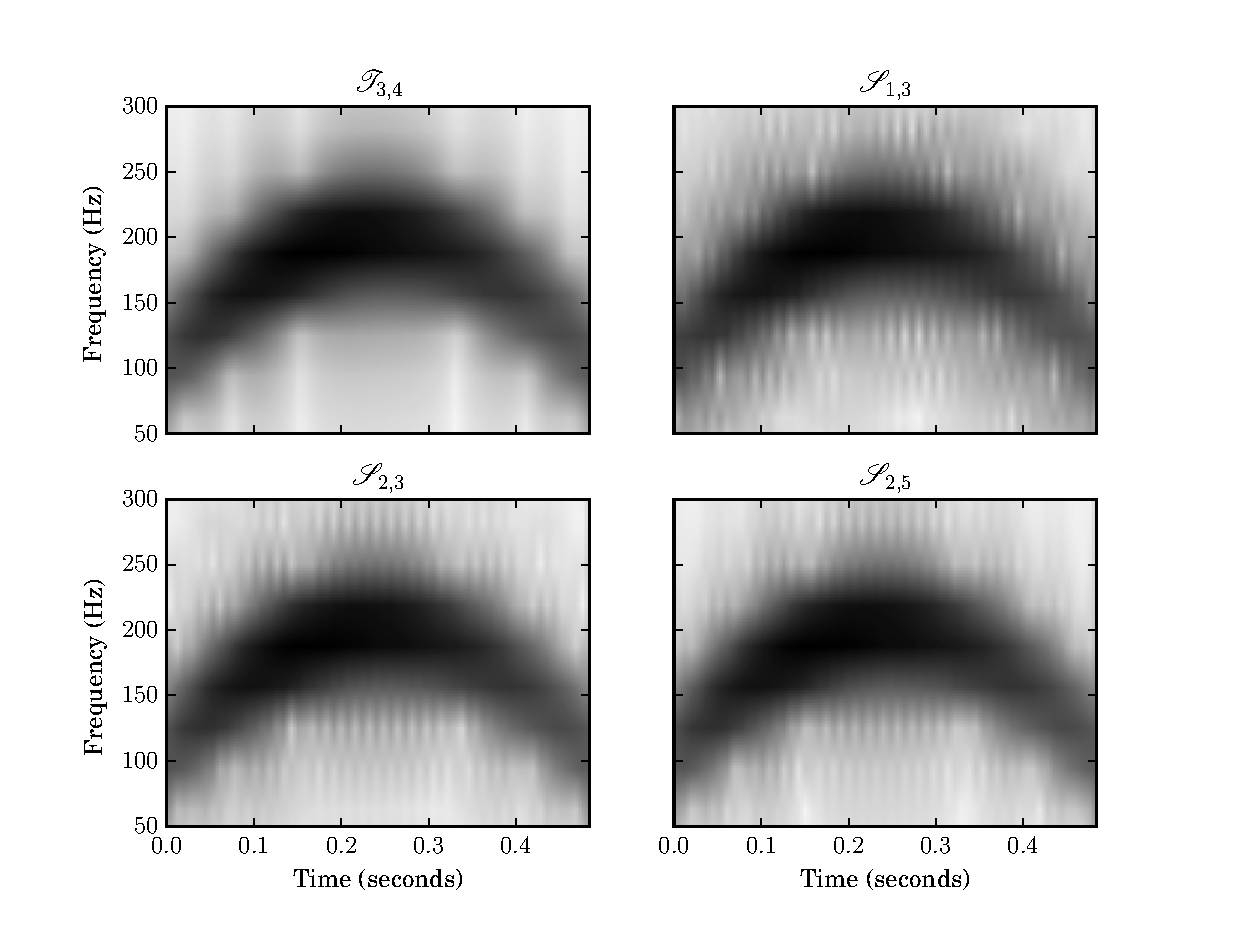
\includegraphics[width=\figwidthscale\textwidth]{plots/mq_mod_err_comp_all_spect.eps}
    \CaptionWithTitle{%
        \input{plots/mq_mod_err_comp_all_spect.txt}%
    }{
        Spectrograms of the true signal and estimated signals for the 
        $\mathscr{T}_{3,4}$ signal.
    \label{plot:mqmoderrorallspect}}
\end{figure}

\begin{figure}[!t]
    \centering
    \includegraphics[width=\figwidthscale\textwidth]{plots/mq_mod_err_comp_true_vs_est_err.eps}
    \CaptionWithTitle{%
        \input{plots/mq_mod_err_comp_true_vs_est_err.txt}%
    }{
        The power of the error when subtracting the original signal from the estimated
        signal. The local upper bound on the error was produced by connecting
        the local maxima in the error data.
    \label{plot:mqerrortruevsesterr}}
\end{figure}

\begin{figure}[!t]
    \centering
    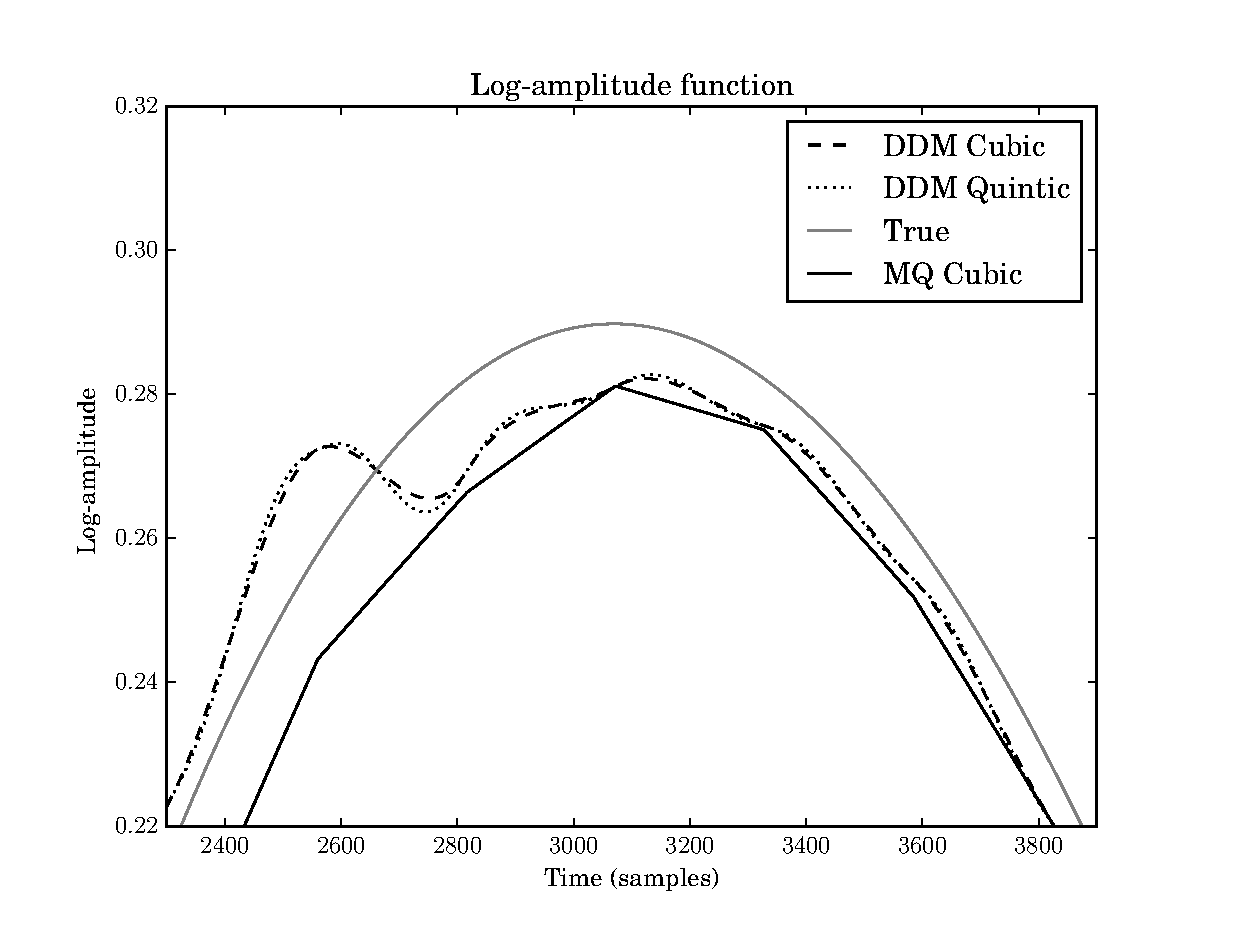
\includegraphics[width=\figwidthscale\textwidth]{plots/mq_mod_err_comp_logamp_func.eps}
    \CaptionWithTitle{%
        \input{plots/mq_mod_err_comp_logamp_func.txt}%
    }{This compares the original log-amplitude function with the
    interpolated log-amplitude functions. The log-amplitude functions are
    considered because these are the real part of the polynomial exponents in
    the complex sinusoid model.
    \label{plot:mqmoderrcomplogampfunc}}
\end{figure}

\begin{figure}[!t]
    \centering
    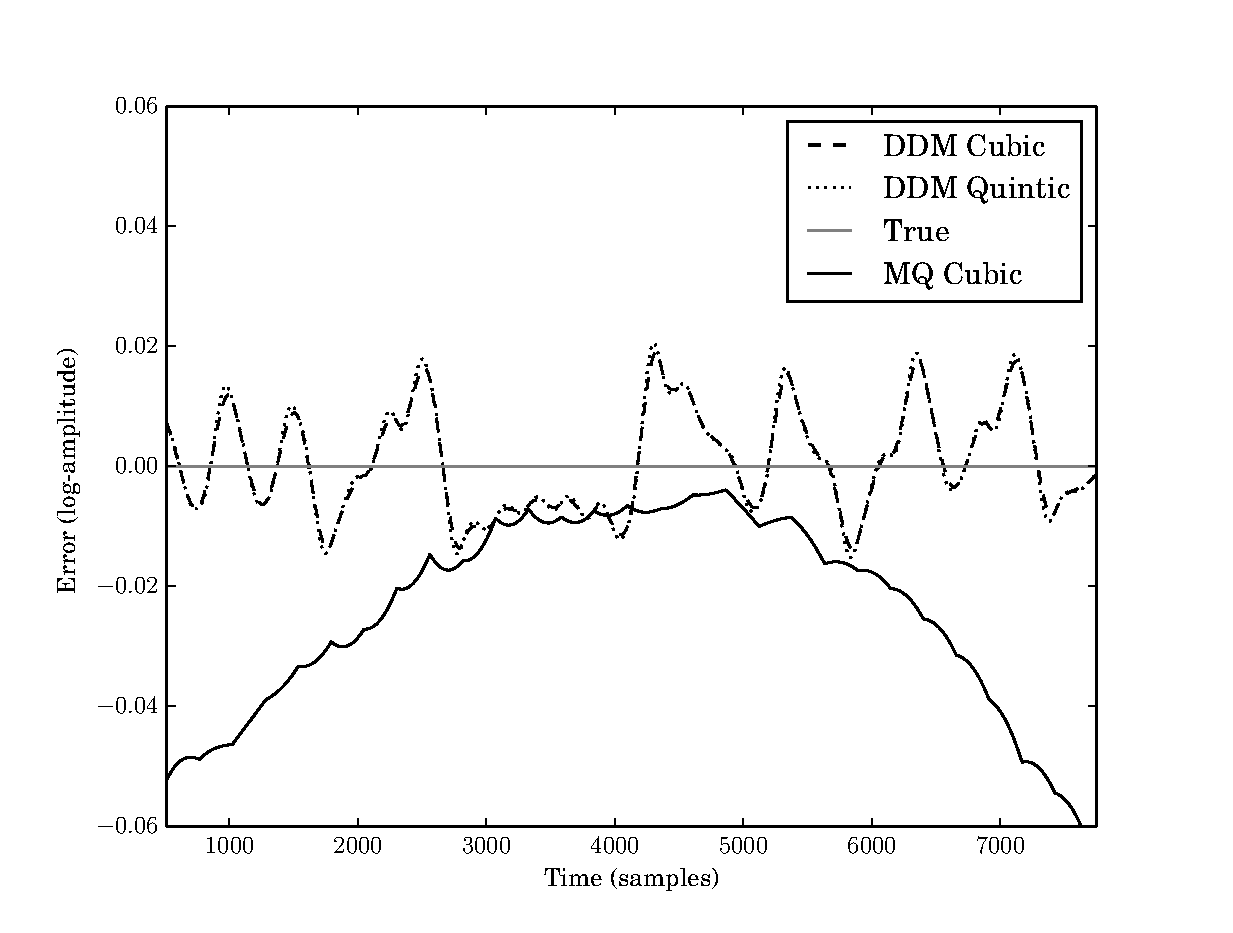
\includegraphics[width=\figwidthscale\textwidth]{plots/mq_mod_err_comp_logamp_err.eps}
    \CaptionWithTitle{%
        \input{plots/mq_mod_err_comp_logamp_err.txt}%
    }{This shows the error of the interpolated log-amplitude functions when compared
    with the original log-amplitude function for the three proposed methods.
    \label{plot:mqmoderrcomplogamperr}}
\end{figure}

\begin{figure}[!t]
    \centering
    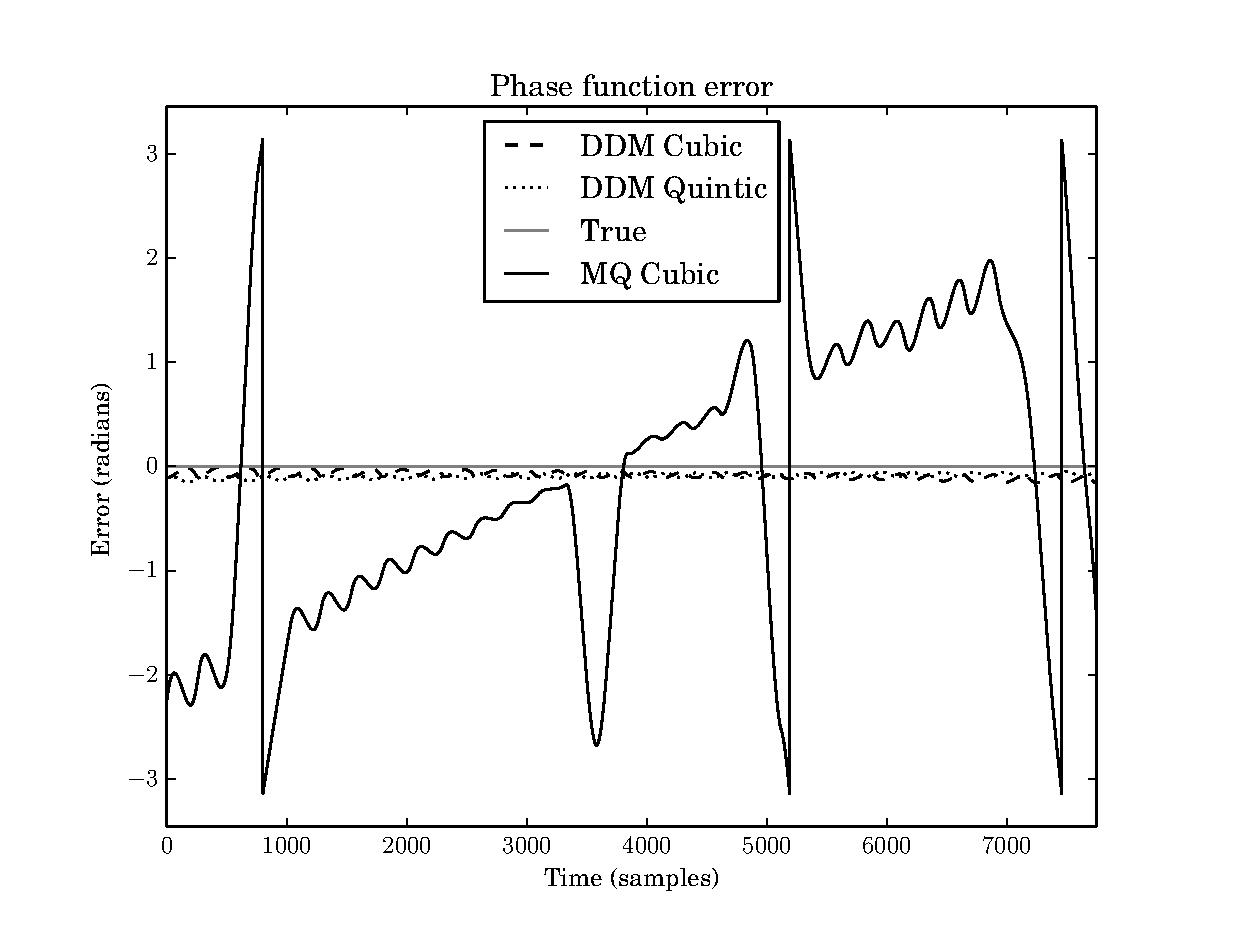
\includegraphics[width=\figwidthscale\textwidth]{plots/mq_mod_err_comp_phase_err.eps}
    \CaptionWithTitle{%
        \input{plots/mq_mod_err_comp_phase_err.txt}%
    }{This compares the theoretical phase function with the interpolated
        phase functions. The phase functions are considered because these are
        the imaginary part of the polynomial exponents in the complex sinusoidal
        model.  The errors are ``wrapped'' to lie between $-\pi$ and $\pi$. The
        errors stem from both the estimation of the phase and the interpolation
        of phase between analysis points. As a frequency modulated sinusoid is
        considered, it is not surprising that the stationary frequency
        assumption of the $\mathscr{S}_{1,3}$ model exhibits the most errors.
    \label{plot:mqmoderrcompphaseerr}}
\end{figure}

The initial evaluation illustrates how higher-order phase and log-amplitude polynomials will not
necessarily improve the quality of synthesis if the underlying phase and
log-amplitude functions are
a polynomial of lower order than the polynomials used for synthesis. As we will
see, the estimated phase and log-amplitude functions suffer from ``overfitting''.

The synthesized signal has 3 frequency break-points and an initial phase,
therefore its phase function can be interpolated by a cubic polynomial
\[
    x_{\phi}(n) = \exp \left(g_3 n^{3} + g_2 n^{2} + g_1 n + g_0 \right)
\]
the frequency break-points are summarized in Table~\ref{tab:cubicsinphparams}. The
initial phase is $0$ radians.

A quartic polynomial is used for the log-amplitude function
\[
    x_{\mu}(n) = \exp \left(h_4 n^{4} + h_3 n^{3} + h_2 n^{2} + h_1 n + h_0 \right)
\]
and its amplitude break-points are summarized in
Table~\ref{tab:quarticsinampparams}. This will be referred to as the
$\mathscr{T}_{3,4}$ signal.

These polynomials are chosen because their orders are greater than or equal to
the order of the synthesis model in the $\mathscr{S}_{2,3}$ system and less than
the order of the synthesis model in the $\mathscr{S}_{2,5}$ system.

The signal was sampled with a sampling rate of 16000 Hz and was analysed every
256 samples with an analysis window of length 1024 samples. For the DDM method, the
$\mathcal{C}^{1}$ 4-Term Blackman-Harris was used (see
Section~\ref{sec:optblackman}).

The results of the evaluation are presented in
Figures~\ref{plot:mqmoderrorallspect}~through~\ref{plot:mqmoderrcompphaseerr}.
In Figure~\ref{plot:mqmoderrorallspect} we see informally that the synthesis
quality is good for all model orders even though the $\mathscr{S}_{1,3}$ model
assumes linear phase in its analysis. Figure~\ref{plot:mqerrortruevsesterr}
shows how accurately the different model orders reconstruct the original signal.
We see that the $\mathscr{S}_{2,5}$, although of higher-order, is not systemically a
better interpolator of the true underlying signal.
Figure~\ref{plot:mqmoderrcomplogampfunc} shows the estimated log-amplitude functions
along with the original and Figure~\ref{plot:mqmoderrcomplogampfunc} their
respective errors in approximating the true log-amplitude function.  Finally,
Figure~\ref{plot:mqmoderrcompphaseerr} shows that the models incorporating the
non-stationary assumption in their analysis perform better at approximating the
true phase function. 

%\begin{figure}[!t]
%    \centering
%    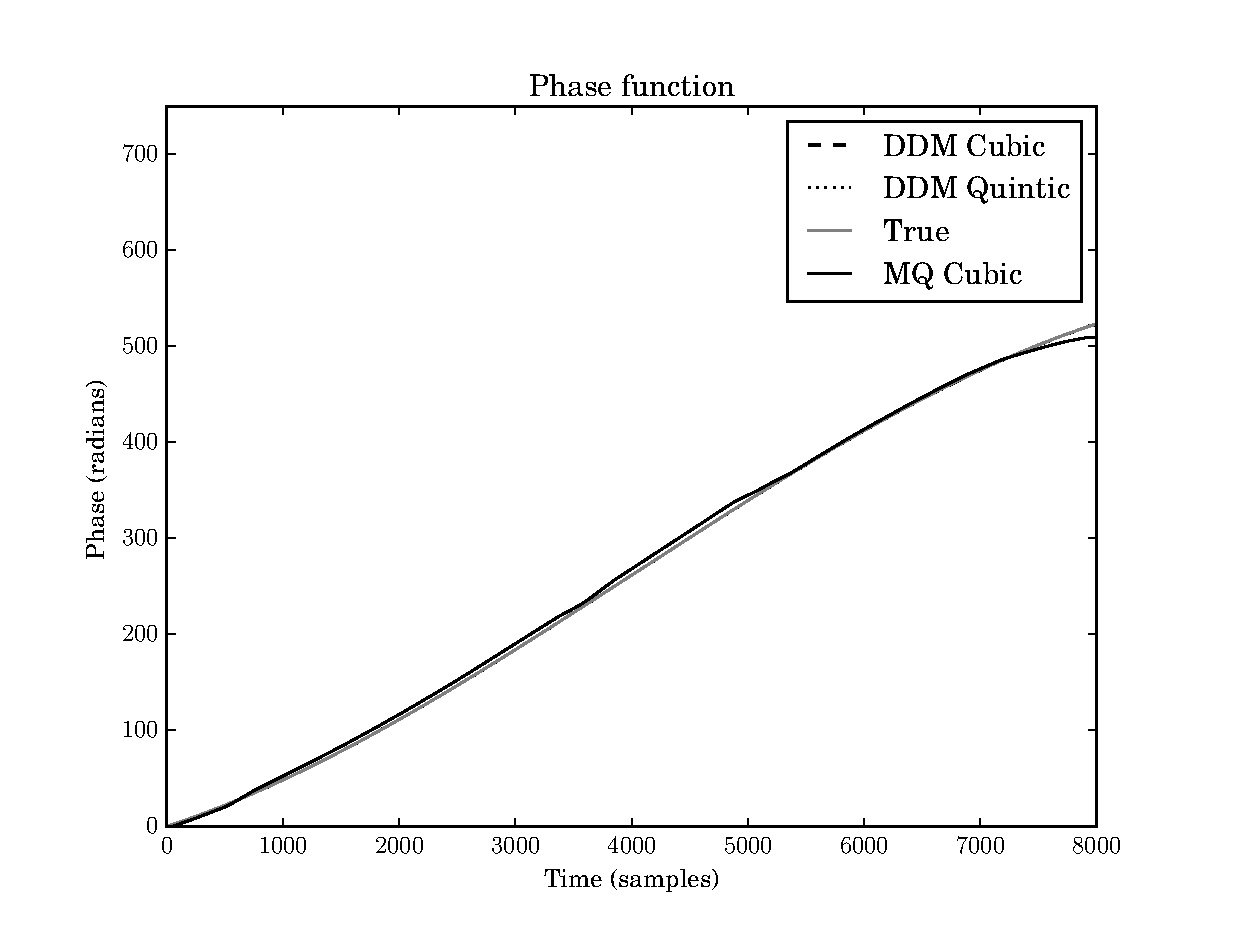
\includegraphics[width=\figwidthscale\textwidth]{plots/mq_mod_err_comp_phase_func.eps}
%    \caption{Error bound of polynomial evaluation using Horner's method. The
%    error bound is shown for the quintic phase and amplitude polynomials.
%    \label{plot:mqmoderrcompphasefunc}}
%\end{figure}

\subsection{Evaluation on sinusoid of exponential phase \label{sec:evalexpphase}}

\begin{figure}[!t]
    \centering
    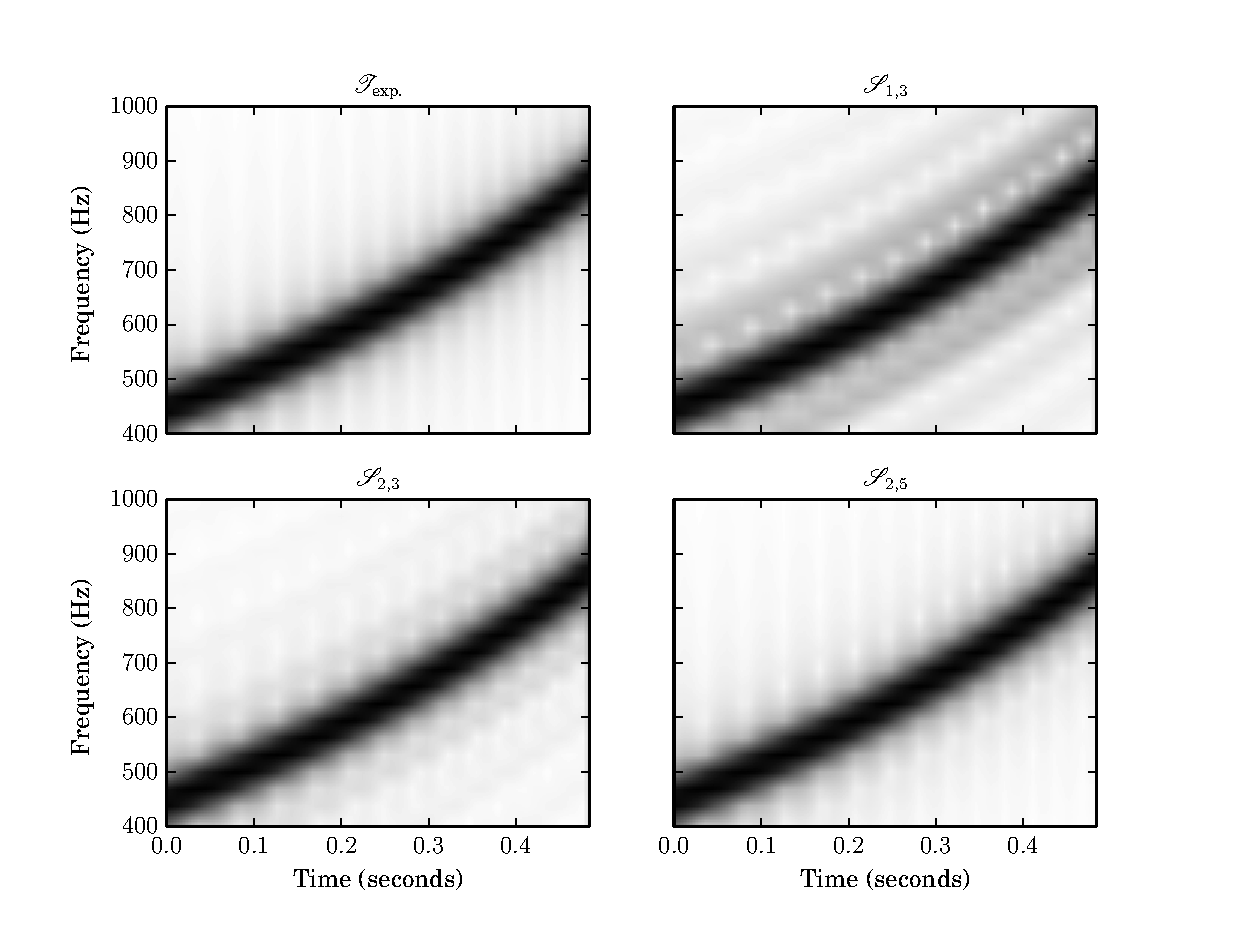
\includegraphics[width=\figwidthscale\textwidth]{plots/mq_exp_err_comp_all_spect.eps}
    \CaptionWithTitle{%
        \input{plots/mq_exp_err_comp_all_spect.txt}%
    }{
        Spectrograms of the true signal and estimated signals for the
        exponential phase signal.
    \label{plot:mqexperrorallspect}}
\end{figure}

\begin{figure}[!t]
    \centering
    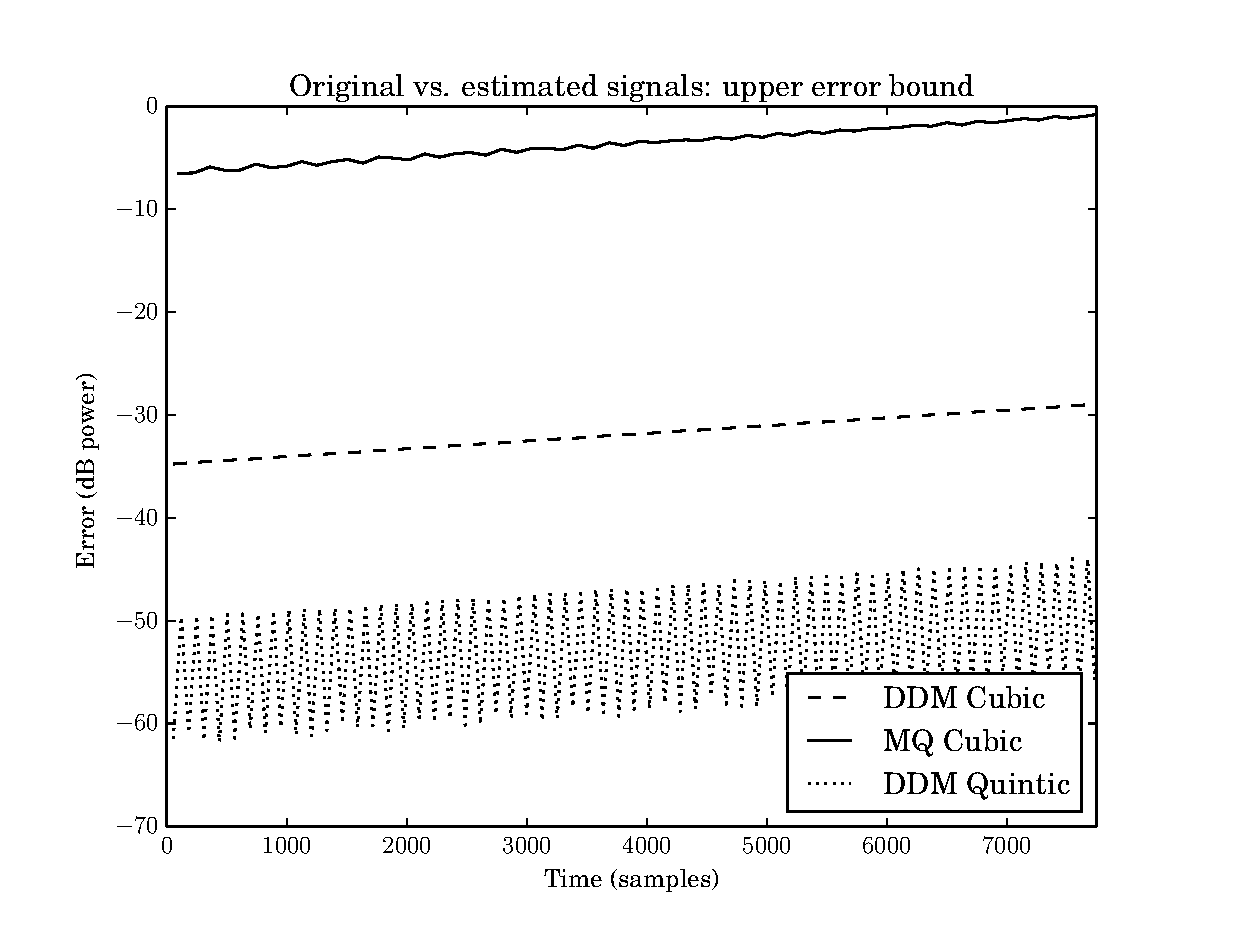
\includegraphics[width=\figwidthscale\textwidth]{plots/mq_exp_err_comp_true_vs_est_err.eps}
    \CaptionWithTitle{%
        \input{plots/mq_exp_err_comp_true_vs_est_err.txt}%
    }{
        The power of the error when subtracting the original signal from the
        estimated signal for the signals of exponential phase. The local upper
        bound on the error was produced by connecting the local maxima in the
        error data.
    \label{plot:mqexperrortruevsesterr}}
\end{figure}

The previous evaluation of this analysis-synthesis system was on a sinusoid with
small order polynomial phase and log-amplitude. In the cases where we observed overfitting, the
polynomial used for synthesis was of higher-order than the true underlying one
--- the interpolating polynomials were more times differentiable than the true
polynomial. We propose evaluating the system on an infinitely differentiable and
analytic phase function. The rationale behind this stems from the definition of
an analytic function: one whose power series representation (a polynomial)
converges to the function as the number of terms approaches infinity. What this
means is, in the region of convergence, the larger the number of terms in the
approximating polynomial, the better the approximation to the true underlying
function. The exponential function
\[
    y=\exp(x), x,y \in \mathbb{R}
\]
is one such function whose power series is
\[
    \exp(x)=\sum_{n=0}^{\infty} \frac{x^{n}}{n!}
\]
To find the radius of convergence, we use the ratio test
\[
    \lim_{n \rightarrow \infty} \frac{|1/n!|}{|1/(n+1)!|} = \lim_{n \rightarrow \infty} n = \infty
\]
i.e., the power series of the exponential function converges everywhere and so
using more terms of its power series will improve its approximation for
any $x \in \mathbb{R}$.

The exponential function arises in music. In 12-tone equal temperament tuning,
to find the frequency $f_{1}$ of a pitch $b$-semitones away from the frequency
$f_{0}$ we compute
\[
    f_{1}=f_{0}2^{\frac{b}{12}}=f_{0}\exp(\log(2)\frac{b}{12})
\]
So a linear transition from pitch $b_{0}$ to $b_{1}$ (in semitones) is an
exponential change in frequency. This could be observed in recordings of
performances of the \textit{portamento} gesture.

We synthesize a sinusoid  of length $N$ samples with exponential phase and use
the same analysis system as in Section~\ref{sec:evalcubicphase} to evaluate the
synthesis accuracy for piece-wise interpolating polynomials of cubic and quartic
order for phase. The signal $x$ is defined
\[
    x(n) = \exp(j\frac{2\pi f_{0}}{c_{1}}\exp(c_{1}n + c_{0}))
\]
with
\[
    c_{0} = \log(2)\frac{b_{0}}{12}
\]
and
\[
    c_{1}= \log(2)\frac{b_{1}}{12N}
\]
i.e., a signal starting at pitch $b_{0}$ with frequency $f_{0}$ and arriving at
pitch $b_{1}$ in $N$ samples. We keep the amplitude of the signal constant in
this evaluation as we are interested in the accuracy of the phase
reconstruction. The same procedure as in
Section~\ref{sec:evalcubicphase} is used to estimate the parameters of
piece-wise interpolating phase polynomials. We can see in
Figure~\ref{plot:mqexperrortruevsesterr} that the resynthesis accuracy is
greater for higher-order polynomials. Spectrograms of the original and estimated
signals are plotted in Figure~\ref{plot:mqexperrorallspect}.

\section{Conclusion}

\subsection{Polynomial phase and log-amplitude function}

Out of the three proposed methods it appears that the modified cubic
interpolation method works superiorly for the signal model considered. We observe
overfitting by the higher-order quintic model in
Figure~\ref{plot:mqmoderrcomplogampfunc}, compromising the accuracy of
resynthesis.  Even the proposed cubic model shows some overfitting in this case.
This is consistent with the results of \cite{girin2003comparing}. From
Figure~\ref{plot:mqmoderrcompphaseerr} it is clear that the DDM based methods
provide superior estimation of the phase function --- this is not the case for
the log-amplitude function. Depending on the underlying signal, perhaps better
results can be obtained by postulating a lower-order log-amplitude function and
higher-order phase function. The possibility of errors arising from numerical
accuracy when evaluating the quintic polynomials has been ruled out.  We
evaluated these polynomials using an implementation of Horner's method that
keeps track of the error bound \cite[p.~95]{higham2002accuracy}: the errors are
negligible, see Figure~\ref{plot:mqmodquinticpolyevalerr} for the results.

\begin{figure}[!t]
    \centering
    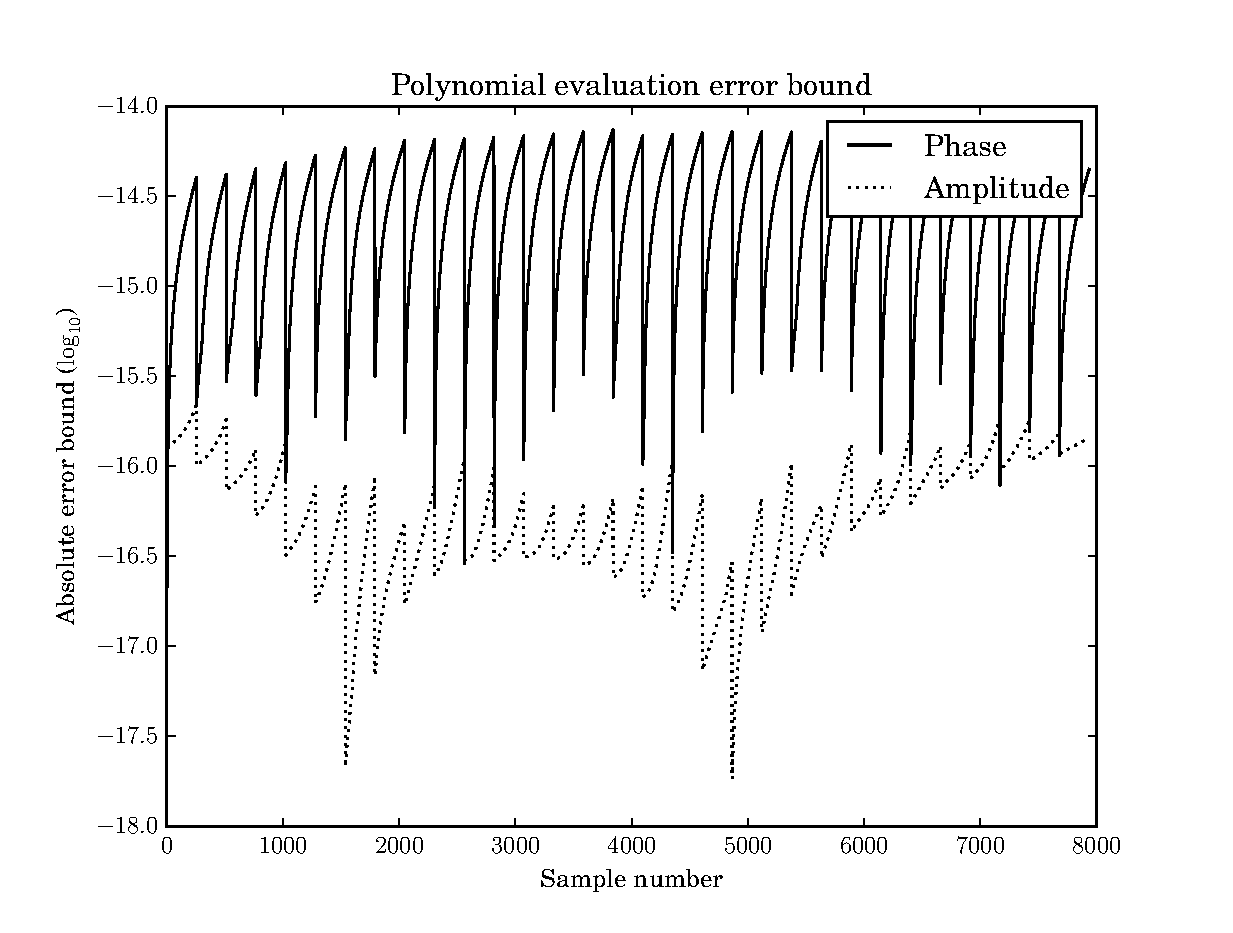
\includegraphics[width=\figwidthscale\textwidth]{plots/mq_mod_quintic_poly_eval_err.eps}
    \CaptionWithTitle{%
        \input{plots/mq_mod_quintic_poly_eval_err.txt}%
    }{The error bound in evaluating the quintic log-amplitude and phase
        polynomials of $\mathscr{S}_{2,5}$ using Horner's method. This plot was produced by plotting only
    the local maxima of the error bound data in order to reduce the plot's
    range.\label{plot:mqmodquinticpolyevalerr}}
\end{figure}

\subsection{Exponential phase function}

The quintic interpolation $\mathscr{S}_{2,5}$, the polynomial of highest order,
performs the most accurate resynthesis. This is consistent with the analytic
property of the exponential function and an encouraging result as it suggests
analytic phase functions can be approximated with arbitrary accuracy simply by
increasing the order of the interpolating polynomials. Many models of musical
gestures involve such functions, apart from the portamento gesture modeled by an
exponential phase function, vibrato can be modeled as a sinusoid with sinusoidal
phase \cite{maher1990investigation}. The DDM-based analysis system combined with
the higher-order polynomial phase and log-amplitude synthesis system presented here
allows for accurate modeling of these gestures.


\chapter{Experiment 2: Partial grouping in one frame}

\section{Introduction}
To evaluate whether the grouping of partials with common AM and FM parameters is
plausible, we synthesize a set of parameters and test by corrupting the
parameters with noise and adding spurious sets of parameters that should not
belong to any sources.

\section{Methodology}
We assume parameters have been estimated already so we start from theoretical
values for the amplitude, frequency, frequency modulation and amplitude
modulation.  On each frame of analysis data, i.e., for parameters belonging to
the same time instant, we consider each data-point as a multi-dimensional random
variable. With these random variables, we compute principal components in order
to produce a variable with maximum variance. This variable is classified using a
clustering algorithm and we evalutate the results. A summary follows:
\begin{itemize}
    \item 
        Parameters are synthesized from a theoretical mixture of AM and FM
        sinusoids.  Spurious data are added to these parameters.
    \item
        Principal components analysis is carried out on the parameters happening
        at one time instance.
    \item
        A histogram is made of the 1st principal components. Values sharing a
        bin with too few other values are discarded to remove spurious data
        points.
    \item
        Initial means and standard deviations for the Gaussian mixture models
        are made by dividing the histogram into equal parts by area and choosing
        the centres of these parts.
    \item
        The EM algorithm for Gaussian mixture models is carried out to classify
        the sources.
\end{itemize}
\section{Evaluation}
The algorithm is run on a typical source separation problem to evaluate its
plausibility.
\section{Synthesis}
Our model makes available the following parameters. Time values are in seconds,
frequency values are in $Hz$ and phase values are in radians.
\begin{itemize}
    \item
        $t$ time.
    \item
        $f_{s}$ sampling frequency.
    \item
        $N$ length of signal in samples.
    \item
        $H$ duration between data-point calculations in samples (i.e., the hop
        size).
    \item
        $N_{p}$ number of sources.
    \item
        $p$ which source.
    \item
        $f_{0,p}$ fundamental frequency.
    \item
        $K_{p}$ number of harmonics.
    \item
        $k_{60,p}$ harmonic number 60 dB lower than the first.
    \item 
        $B_{p}$ the inharmonicity coefficient.
    \item
        $\phi_{0,p}$ initial phase.
    \item
        $\phi_{0,f,p}$ initial FM phase.
    \item
        $t_{60,p}$ time until amplitude of partial has dropped 60 dB.
    \item
        $t_{\text{attack},p}$ time duration of attack portion.
    \item
        $A_{f,p}$ amplitude of FM.
    \item
        $f_{f,p}$ frequency of FM.
    \item
        $s_{p}$ the signal representing the $p$th source.
\end{itemize}

To incorporate inharmonicity often observed in real string instruments where the
strings exhibit some stiffness, we define the \textit{stretched} harmonic numbers
as follows
\cite{paspweb2010}\footnote{
\texttt{http://ccrma.stanford.edu/\~{}jos/pasp/Dispersion\_Filter\_Design\_I.html}}

\begin{equation}
    K_{B}(k) = k (1+Bk^{2})^{\frac{1}{2}}
\end{equation}

Each source is synthesized using the following equation:
\begin{equation}
    s_{p}(t) = \sum_{k=1}^{K_{p}} A_{p}(k,t) \exp(j(2\pi
    f_{0,p}t - \frac{A_{f,p}}{f_{f,p}} \cos(2\pi f_{f,p} t +
    \phi_{0,f,p}) K_{B_{p}}(k) + \phi_{0,p}))
\end{equation}
where
\begin{equation}
    A_{p}(k,t) = 
    \begin{cases}
        \exp(a_{60,p} t + a_{k,60,p}k) \cos^{2}
        (\frac{\pi}{2}(\frac{t}{t_{\text{attack},p}} - 1)) & \text{if } t \leq
        t_{\text{attack},p},\\
        \exp(a_{60,p} t + a_{k,60,p}k) & \text{if } t > t_{\text{attack},p},\\
        0 & \text{otherwise}.
    \end{cases}
\end{equation}
\begin{equation}
    a_{60,p} = \frac{\log(10^{-3})}{t_{60,p}}
\end{equation}
\begin{equation}
    a_{k,60,p} = \frac{\log(10^{-3})}{k_{60,p}} 
\end{equation}
The piecewise amplitude function is based on the amplitude function of the
\textit{Formant Wave Function (FOF)}\footnote{FOF stands for \textit{Forme
d'Onde Formantique}.} described in \cite[p.~19]{rodet1984chant}.

The estimation of these parameters is a separate problem addressed by the
DDM (see Section~\ref{sec:ddm_description}). We use theoretical values calculated
directly from the model signals. For interpretation, and to make it possible to
simply replace the theoretical values with those obtained from an analysis, we
compute parameters that correspond to the model of these methods.

The DDM seeks signals $s_k \in \mathbb{C}$ of the following form:
\begin{equation}
    s_{k}(n) = \exp(\log(A_{k}) + \alpha_{k}n + j(\phi_{k} + \omega_{k}n +
    \frac{1}{2} \psi_{k} n^{2})) \label{eq:rm_model}
\end{equation}
Here $n$ is the sample number. Typically when performing a short-time analysis,
the time corresponding to $n = 0$ is made to be the centre of the window,
therefore, $t$ is the time at the centre of the window and $N_{w}$, in samples,
is the length of the middle (usually non-zero) portion of the window. The
coefficents of the $k$th harmonic of the $p$th source from our synthetic model
are given by
\begin{equation}
    \alpha_{k,p}(t) = \frac{a_{60,p}}{f_{s}}
\end{equation}
\begin{equation}
    A_{k,p}(t) = \exp(a_{60,p} t + a_{k,60,p} k)
\end{equation}
for the part of the signal after the attack portion.

For the attack portion, we estimate the parameters using least-squares on a
rectangular-windowed signal. Let
\begin{equation}
    \hat{\mathbf{s}}_{k,p}(t) =
    \begin{pmatrix}
        \exp \left(\displaystyle a_{60,p} \left( t - \frac{N_{w}}{2f_{s}} \right)  +
        a_{k,60,p} k \right) \cos^{2} \left(\displaystyle \frac{\pi}{2} \left(
                \frac{ t
        - \frac{N_{w}}{2f_{s}} }{ t_{\text{attack},p}} - 1 \right) \right)  \\
        \vdots \\
        \exp \left(\displaystyle a_{60,p} \left( t + \frac{N_{w}}{2f_{s}} \right)  +
        a_{k,60,p} k \right) \cos^{2} \left(\displaystyle \frac{\pi}{2} \left(
                \frac{ t
        + \frac{N_{w}}{2f_{s}}  }{ t_{\text{attack},p}} - 1 \right) \right)
    \end{pmatrix}
\end{equation}
then $\log(A_{k,p})$ and $\alpha_{k,p}$ are found as the least-squares solution of
\begin{equation}
    \begin{bmatrix}
        1 & \frac{-N_{w}}{2} \\
        \vdots & \vdots \\
        1 & \frac{N_{w}}{2}
    \end{bmatrix}
    \begin{pmatrix}
        \log(A_{k,p}(t)) \\
        \alpha_{k,p}(t)
    \end{pmatrix}
    = \log{\hat{\mathbf{s}}_{k,p}(t)}
\end{equation}

for the argument parameters (those multiplied by $j$ in Equation~\eqref{eq:rm_model})

\begin{equation}
    \omega_{k,p} \left( t \right)  = \frac{2 \pi}{f_{s}}  \left(  f_{0,p} +
    A_{f,p} \sin \left( 2 \pi f_{f,p} t + \phi_{0,f,p} \right)  \right)
    K_{B_{p}} \left( k \right) 
\end{equation}
\begin{equation}
    \psi_{k,p} \left( t \right)  =  \left( \frac{2 \pi}{f_{s}} \right) ^{2}
    A_{f,p} f_{f,p}  \left(  f_{0,p} + A_{f,p} \cos \left( 2 \pi f_{f,p} t +
    \phi_{0,f,p} \right)  \right)  K_{B_{p}} \left( k \right) 
\end{equation}
\begin{equation}
    \phi_{k} \left( t \right)  =  \left( 2\pi f_{0,p}t - \frac{A_{f,p}}{f_{f,p}}
    \cos \left( 2\pi f_{f,p} t + \phi_{0,f,p} \right)  \right)  K_{B_{p}} \left(
    k \right)  + \phi_{0,p}
\end{equation}

To simulate the noise that would be present in an estimation of the signal
parameters from an arbitrary signal, we create noise corrupted values by
substituting the random variables:
\begin{itemize}
    \item
        $\tilde{\Psi}_{k,p}(t) \sim
        \mathcal{N}(\psi_{k,p}(t),\psi_{no})$
    \item
        $\tilde{\Omega}_{k,p}(t) \sim
        \mathcal{N}(\omega_{k,p}(t),\omega_{no})$
    \item
        $\tilde{\alpha}_{k,p}(t) \sim
        \mathcal{N}(\alpha_{k,p}(t),\alpha_{no})$
    \item
        $\tilde{A}_{k,p}(t) \sim
        \mathcal{N}(A_{k,p}(t),A_{no})$
\end{itemize}
%% If using correlated random variables
%\begin{itemize}
%    \item
%        $\tilde{\Psi}_{k,p}(t) \sim
%        \mathcal{N}(\psi_{k,p}(t),\psi_{no})$
%    \item
%        $\tilde{\Omega}_{k,p}(t) \sim
%        \mathcal{N}(\omega_{k,p}(t),\omega_{no})
%        + \tilde{\psi}_{k,p}(t-\Delta t) \Delta t)$
%    \item
%        $\tilde{\Phi}_{k,p}(t) =
%        \tilde{\omega}_{k,p}(t - \Delta t) \Delta t$
%    \item
%        $\tilde{\alpha}_{k,p}(t) \sim
%        \mathcal{N}(\alpha_{k,p}(t),\alpha_{no})$
%    \item
%        $\tilde{A}_{k,p}(t) \sim
%        \mathcal{N}(A_{k,p}(t),A_{no})$
%\end{itemize}
The $\theta_{no}$ (where $\theta$ is replaced by $\omega$ etc.) specifies the
variance of the particular parameter. Most-likely in practice these random
variables would be correlated but not knowing the estimation method, we cannot
at this point say anything about this correlation. Therefore the noisy
parameters are uncorrelated random variables for this experiment.

We also add spurious data-points as a fraction $r$ of the number of true
data-points.  Their values are drawn from uniform distributions with boundaries
$\theta_{\text{min}}$ and $\theta_{\text{max}}$, where $\theta$ is some
parameter above, e.g., $\omega_{\text{min}}$ and $\omega_{\text{max}}$ for the
$\omega$ parameter. For this experiment $r = 0.25$. The parameters of the
uniformly distributed random variables are given in
Table~\ref{tab:amfmspuriousuniformparams}.
\begin{table}
    \caption{Comparison of total costs\label{tab:amfmspuriousuniformparams}}
    \begin{center}
        \begin{tabular}{l r r}
            Parameter & $\theta_{\text{min}}$ & $\theta_{\text{max}}$ \\
            \hline
            $\omega$  & $0$ & $\pi$ \\
            $\psi$    & $-1 \times 10^{-4}$ & $1 \times 10^{-4}$ \\
            $\alpha$    & $-1 \times 10^{-3}$ & $1 \times 10^{-3}$ \\
        \end{tabular}
    \end{center}
\end{table}
Data points are computed for the times $t = 0,\frac{H}{f_{s}},\frac{2
H}{f_{s}},\ldots,\frac{\left\lfloor \frac{N}{H} \right\rfloor H}{f_{s}}$.

\section{Computation of Principal Components}

At each time $t$ we have $L$ data-points. As the source of each data-point is
now unknown, we replace the $k$ and $p$ indices with index $l$. We only consider
the amplitude and frequency modulation. According to our model, the frequency
modulation is greater for harmonics of greater centre frequency. To take this
into consideration, we divide the frequency modulation estimate $\psi_{l}(t)$ by
the constant frequency estimate $\omega_{l}(t)$. This is similar to the approach
taken in \cite{creager2016musicalsource}. The amplitude modulation $\alpha_{l}(t)$
remains constant for all harmonics of the same source, only its initial value
changes according to $k_{60,p}$.  We compile the data-points at one time into a
set of observations.
\begin{equation}
    \mathbf{x}_{l}(t) = \begin{pmatrix}
        \frac{\psi_{l}(t)}{\omega_{l}(t)} \\
        \alpha_{l}
    \end{pmatrix}
\end{equation}
\begin{equation}
    \mathbf{X}(t) = \begin{bmatrix}
        \mathbf{x}_{1}(t) \ldots \mathbf{x}_{L}(t)
    \end{bmatrix}
\end{equation}
From these $L$ observations the correlation matrix $\mathbf{S}$ is computed. We
use the correlation matrix because the values in each row of $\mathbf{x}_{l}(t)$
do not have the same units, see \cite[p.~22]{jolliffe2002principal} for a
discussion about this. 

Following the standard technique for producing principal components
\cite[p.~11]{jolliffe2002principal}, we obtain a matrix $\mathbf{V}(t)$ of
eigenvectors sorted so that the eigenvector corresponding to the largest
eigenvalue is in the first column, etc.  The principal components
$\mathbf{A}(t)$ are then computed as
\begin{equation}
    \mathbf{A}(t) = \mathbf{V}^{T}(t)\mathbf{X}(t)
\end{equation}
We have found it sufficient to use only the first principal component and
therefore only use the values in the first row of $\mathbf{A}(t)$

If we see the $\mathbf{x}_{l}(t)$ as realizations of a random variable, the
above computation of principal components has the effect of projecting
realizations of $\mathbf{x}_{l}(t)$ to points $a_{1,l}(t)$ on a 1-dimensional
subspace. It is a fundamental theory of principal components that the
transformation above maximizes the expected euclidean distance between the
points $a_{1,l}(t)$. This is desirable for the current problem because it will
always produce a variable emphasizing the parameter with the most variance,
hence if we are observing a random variable drawn from multiple distributions
with sufficiently separated means and small enough variances, this separation
will be most observable in the principal components corresponding to the
greatest eigenvalues.

\section{Preparing data for clustering \label{sec:amfmseppreparecluster}}
The Expectation Maximization underlying the Gaussian mixture model parameter
estimation will only converge to a local maximum (see Dempster et al),
therefore, for the best results, we compute a good initial guess and remove
obvious outliers before carrying out the clustering algorithm.

The $a_{1,l}(t)$ are compiled into a histogram of $N_{b}$ bins. The minimum and
maximum bin boundaries are computed from the maximum and minimum values of
$a_{1,l}(t)$ respectively. Values in a bin with less than $\tau_{h}$ other
values are discarded. We find $N_{p}$ contiguous sections of equal area in the
new histogram omitting the discarded values.  We use the centres of these
sections as the initial mean guesses and half their width as the distance 3
standard deviations from the mean (roughly 99.7 percent of values drawn from one
distribution will lie within this interval if they indeed follow a normal
distribution). The initial guesses for the weights are simply $\frac{1}{N_{p}}$.

\section{Clustering}
GMM parameter estimation is discussed in Section~\ref{sec:gmm}. After
convergence we have an estimated probability $p(a_{1,l}(t) \text{ from
distribution }p)$. We choose the distribution $p$ for each $a_{1,l}(t)$ that
gives the highest probability of it having occured. The values
$\mathbf{x}_{t}(t)$ corresponding to the $a_{1,l}(t)$ have this same
classification. Those sharing the same classification can be interpreted as
coming from the same source. The figure shows the results of the above steps
carried out on a mixture of two sources synthesized with the 
parameters summarized in Table~\ref{tab:synthparamamfmsep}.
\begin{table}
    \begin{center}
        \begin{tabular}{c c c }
            Parameter & Source 1 value & Source 2 value \\
            \hline
            $f_{0,p}$ & 261.63 & 277.18 \footnote{These are the fundamental
            frequencies of a $c_{4}$
            and $c_{4}^{\sharp}$ respectively.} \\
            $K_{p}$ & 20 & 20 \\
            $k_{60,p}$ & 20 & 20 \\
            $B_{p}$ & 0.001 & 0.001 \\
            $\phi_{0,p}$ & 0 & 0 \\
            $\phi_{0,f,p}$ & 0 & 0.8 \\
            $t_{60,p}$ & 0.5 & 0.75 \\
            $t_{\text{attack},p}$ & 0.1 & 0.1 \\
            $A_{f,p}$ & 7.666 & 8.1220 \footnote{These values are found by
            computing $f_{0,p}2^{1/24}-f_{0,p}$ giving a quarter-tone of
            frequency modulation centred around the fundamental frequency.} \\
            $f_{f,p}$ & 3 & 2
        \end{tabular}
    \end{center}
    \caption{Synthesis parameters for source separation by frequency and
    amplitude modulation. \label{tab:synthparamamfmsep}}
\end{table}
The length of the signal $N$ is 8000 samples and the anlaysis hop size $H$ is 256
samples. The figures in \ref{sec:amfmsepresults} summarize the results of the
source separation experiment.

%\begin{figure}[!t]
%    %\centering
%\includegraphics[width=\textwidth]{/home/sandman/Documents/development/masters_thesis/experiment_1/plots/time_frequency_spurious.ps}
%\end{figure}
\section{Results \label{sec:amfmsepresults}}

% Plots produced in this section with signal_modeling/test/plot_all_am_fm_sep.sh

Here we show source separation results for the synthesized signals with varying
amounts of noise added to the synthesis parameters $\psi$, $\omega$, $\alpha$
and $A$. The amount of noise added and the corresponding plot title is
summarized in Table~\ref{tab:amfmexpplotkey}.

\begin{table}
    \begin{center}
        \begin{tabular}{l c c c c}
            Table number & $\psi_{no}$ & $\omega_{no}$ & $\alpha_{no}$ &
            $A_{no}$ \\
            \hline
            1 & $1 \times 10^{-2}$ & $1 \times 10^{-2}$ & $1 \times 10^{-2}$ &
            $1 \times 10^{-4}$ \\
            2 & $1 \times 10^{-2}$ & $1 \times 10^{-2}$ & $1 \times 10^{-2}$ &
            $1 \times 10^{-5}$ \\
            3 & $1 \times 10^{-3}$ & $1 \times 10^{-3}$ & $1 \times 10^{-3}$ &
            $1 \times 10^{-4}$ \\
            4 & $1 \times 10^{-3}$ & $1 \times 10^{-3}$ & $1 \times 10^{-3}$ &
            $1 \times 10^{-5}$ \\
        \end{tabular}
    \end{center}
    \caption{\label{tab:amfmexpplotkey}}
\end{table}

\begin{figure}[!t]
    %\centering
    \includegraphics[width=\textwidth]{plots/{hsrp_test_7_multi_orig_data}.eps}
    \caption{Line-segments describing the frequency and frequency modulation
    of both sources.\label{plot:hsrp_test_7_multi_orig_data}}
\end{figure}

\begin{figure}[!t]
    %\centering
    \includegraphics[width=\textwidth]{plots/{hsrp_test_7_multi_orig_spur_data}.eps}
    \caption{Line-segments describing the frequency and frequency modulation
        of the original data and the spurious data.
    \label{plot:hsrp_test_7_multi_orig_spur_data}}
\end{figure}

\begin{figure}[!t]
    %\centering
    \includegraphics[width=\textwidth]{plots/{hsrp_test_7_multi_class_pcs}.eps}
    \caption{The PCs for each theoretical analysis time-point. $\mu_{i}^{0}$ and
        $\sigma_{i}^{0}$ are respectively
    the initial mean and standard deviation guesses for the EM algorithm fitting
    the GMM parameters to the $i$th source. These values are also visible on the
    plot. The spurious points rejected using the process described in
    Section~\ref{sec:amfmseppreparecluster} are included for comparison. The
    plot is of a subsection of the analysis to better show the process.
    \label{plot:hsrp_test_7_multi_class_pcs}}
\end{figure}

\begin{figure}[!t]
    %\centering
    \includegraphics[width=\textwidth]{plots/{hsrp_test_7_multi_source_1_est}.eps}
    \caption{Line-segments classified as belonging to Source 1. The
        classification is done on each frame so classifications in consecutive
        frames may not belong to the same true source. This is because the
        ordering of the clusters in each frame in
        Figure~\ref{plot:hsrp_test_7_multi_class_pcs} is not predictible.
    \label{plot:hsrp_test_7_multi_source_1_est}}
\end{figure}

\begin{figure}[!t]
    %\centering
    \includegraphics[width=\textwidth]{plots/{hsrp_test_7_multi_source_2_est}.eps}
    \caption{Line-segments classified as belonging to Source 2. See
        Figure~\ref{plot:hsrp_test_7_multi_source_2_est} for more
        information.
    \label{plot:hsrp_test_7_multi_source_2_est}}
\end{figure}

As seen in Figure~\ref{plot:hsrp_test_7_multi_source_1_est} and
\ref{plot:hsrp_test_7_multi_source_2_est}, while
classified well in individual frames, the overall classification does not
correspond to a single source. We must find a collection of frames with high
plausibility of belonging to one source. We consider the collections of
classified data-points corresponding to each source as a node in a lattice. Each
frame of the lattice contains two nodes, one for each source. A best path
through the lattice should connect together those nodes belonging to a single
source. We use the results of
Section~\ref{sec:lppathsearch} to find the two best paths through this lattice.
We compare two distance metrics for the cost function.

The first prefers
smoothness in frequency between two frames. For frame $h$ with initial
classification $\tilde{p}$ we have frequency measurements
$\omega_{k,\tilde{p}}^{h}$
and frequency slope measurements $\psi_{k,\tilde{p}}^{h}$. The set of parameters
at time $h$ from initially classified source $\tilde{p}$ we will denote
$\boldsymbol{\theta}_{\tilde{p}}^{h}$. Between frame $h$ and frame $h-1$ we use
Algorithm~\ref{alg:mq_peak_match} on the pairs $\left\{ \boldsymbol{\theta}_{\tilde{m}}^{h},
\boldsymbol{\theta}_{\tilde{n}}^{h+1} \right\}$ with $(m,n) \in \{0,1\} \times
\{0,1\}$. For
each pair, $L$ is set to $\min(\# \boldsymbol{\theta}_{\tilde{m}}^{h} ,
\# \boldsymbol{\theta}_{\tilde{n}}^{h+1}).$\footnote{Here, the threshold parameter $\Delta
= \infty$, i.e., a connection of any cost is possible.} The cost function is the absolute error
in predicting the frequency in the next frame from parameters in the current
frame, i.e.,
\[
    \mathcal{D}_{f} \left( \theta_{i,\tilde{m}}^{h},
    \theta_{j,\tilde{n}}^{h+1} \right) = | \omega_{i,\tilde{m}}^{h} +
    \psi_{i,\tilde{m}}^{h} H - \omega_{j,\tilde{n}}^{h+1} |
\]
where $H$ is the
hop-size in samples between the two frames.
The second distance metric prefers smoothness in amplitude between two frames.
It is given as
\[
    \mathcal{D}_{a} \left( \theta_{i,\tilde{m}}^{h},
    \theta_{j,\tilde{n}}^{h+1} \right) = | \log(A_{i,\tilde{m}}^{h}) +
    \psi_{i,\tilde{m}}^{h} H - \log(A_{j,\tilde{n}}^{h+1}) |
\]
We have found the absolute error to
give better results than the squared error.

The costs of these connections
are summed over the index pairs $\Gamma_{h}$ to give the entries of the cost
vector $\boldsymbol{c}$ in the LP
\[
    \boldsymbol{c}_{4t + 2m + n} = \sum_{i^{\ast},j^{\ast} \in \Gamma_{h}}
    \mathcal{D} \left( \theta_{i^{\ast},\tilde{m}}^{h}, \theta_{j^{\ast},\tilde{n}}^{h+1}
    \right)
\]

The specification of the constraint matrices is done according to the topology
of the lattice and the requirement that we find 2 non-overlapping paths (see
Section~\ref{sec:lppathsearch}). An example of discovered paths is given in
Figure~\ref{plot:hsrp_test_7_multi_smooth_freq_amp_sol}.
\begin{figure}[!t]
    %\centering
    \includegraphics[width=\textwidth]{plots/{hsrp_test_7_multi_smooth_freq_amp_sol}.eps}
    \caption{The points originally classified as source 1 are marked with
        circles and those originally classified as source 2 squares. The paths
        in black or grey connect the points for source 1 or source 2
        respectively with optimal smoothness.
    \label{plot:hsrp_test_7_multi_smooth_freq_amp_sol}}
\end{figure}
The estimated sources after smoothing in frequency are shown in
Figures~\ref{plot:hsrp_test_7_multi_source_1_smooth_freq}~and~\ref{plot:hsrp_test_7_multi_source_2_smooth_freq}
\begin{figure}[!t]
    %\centering
    \includegraphics[width=\textwidth]{plots/{hsrp_test_7_multi_source_1_smooth_freq}.eps}
    \caption{Line-segments classified as belonging to source 1 after smoothing
        in frequency.
    \label{plot:hsrp_test_7_multi_source_1_smooth_freq}}
\end{figure}
\begin{figure}[!t]
    %\centering
    \includegraphics[width=\textwidth]{plots/{hsrp_test_7_multi_source_2_smooth_freq}.eps}
    \caption{Line-segments classified as belonging to source 2 after smoothing
        in frequency.
    \label{plot:hsrp_test_7_multi_source_2_smooth_freq}}
\end{figure}
The estimated sources after smoothing in amplitude are shown in
Figures~\ref{plot:hsrp_test_7_multi_source_1_smooth_amp}~and~\ref{plot:hsrp_test_7_multi_source_2_smooth_amp}
\begin{figure}[!t]
    %\centering
    \includegraphics[width=\textwidth]{plots/{hsrp_test_7_multi_source_1_smooth_amp}.eps}
    \caption{Line-segments classified as belonging to source 1 after smoothing
        in amplitude.
    \label{plot:hsrp_test_7_multi_source_1_smooth_amp}}
\end{figure}
\begin{figure}[!t]
    %\centering
    \includegraphics[width=\textwidth]{plots/{hsrp_test_7_multi_source_2_smooth_amp}.eps}
    \caption{Line-segments classified as belonging to source 2 after smoothing
        in amplitude.
    \label{plot:hsrp_test_7_multi_source_2_smooth_amp}}
\end{figure}
We see that when smoothed in frequency, the results are acceptable. However,
when both sets of parameters are close and give close costs, the spurious
data-points can influence the cost function causing a false classification. This
can be seen at around 0.35 seconds in
Figures~\ref{plot:hsrp_test_7_multi_source_1_smooth_freq}~and~\ref{plot:hsrp_test_7_multi_source_2_smooth_freq}
where it seems perhaps 3 frames should be classified as the other source. That
these are difficult to classify is not surprising, comparing with
Figures~\ref{plot:hsrp_test_7_multi_orig_data} we see that at around
0.38 seconds the frequency slopes are close.

When smoothed in amplitude, the results are less convincing. This is not
surprsing as smoothness in amplitude is not the best criterion at all time
points.
\begin{figure}[!t]
    %\centering
    \includegraphics[width=\textwidth]{plots/{hsrp_test_7_multi_af}.eps}
    \caption{ Line-segments representing the instantaneous amplitude and amplitude slope at
        analysis time points. 
    \label{plot:hsrp_test_7_multi_af}}
\end{figure}
In Figure~\ref{plot:hsrp_test_7_multi_af} we see that the amplitudes of
both sources are similar at many points, e.g., at around 0.05 and 0.15 seconds.
Indeed it is here that the amplitude smoothness criterion fails, as we see in
Figures~\ref{plot:hsrp_test_7_multi_source_1_smooth_amp}~and~\ref{plot:hsrp_test_7_multi_source_2_smooth_amp}.

\section{Conclusion}

In this chapter we evaluated the plausibility of separating two mixed sources
by classifying based on their theoretical frequency and amplitude modulation. We
obtained acceptable results for signals with small measurement errors. The
method is also robust in the presence of spurious data points. A shortcoming of
the method is the requirement that the frequency and frequency modulation of the
signals be known. If the signals are sufficiently separated in frequency and
have small bandwidth, as shown in Section~\ref{sec:ddm_description} the DDM can
be used to estimate these parameters. If signals are close in frequency, the
number of sinusoids is known, and these
exhibit slow modulations, signal subspace methods could be used \cite{} where
the estimations at different time points are connected as in
Section~\ref{sec:partialtracking} and the modulation parameters postulated via
interpolation similarly to Section~\ref{sec:mqfmfromphase}.
% What about initial phase of sinusoids???
Another strategy might be to use two uncorrupted measurements of one source and
extrapolate the parameters of the signal in the part corrupted by the other.
Another shortcoming of the technique presented here is the use of the costly EM
algorithm to classify data points using GMM. A more ad hoc approach could be
taken to save on these computations, perhaps partitioning the data sets using
local maxima as the means and local minima as points some number of standard
deviations away from these means. Were these two drawbacks overcome, the source
separation technique presented here is inexpensive computationally and can even
resolve the phases of the sinusoids, which are discarded in techniques using the
power spectrum such as NMF and PLCA.


\chapter{Experiment: Separation of two sources using partial decay rate
\label{chap:decaysep}}

% plot produced with
% plot_pep_3_3d.py

% plots produced with ../../signal_modeling/test/partial_estimation_plot_3_3c.py

\section{Introduction}

In this section we demonstrate how the techniques described above can be used to
perform audio source separation on signals obtained from recordings of acoustic
instruments. Specifically, we show that in the absence of frequency-modulation,
amplitude modulation --- the decay rate --- can be used to classify partials
in a mixture of two sources into two groups, each group representing an
underlying source.

\section{Description of problem}

\begin{figure}%[t]
    \centering
    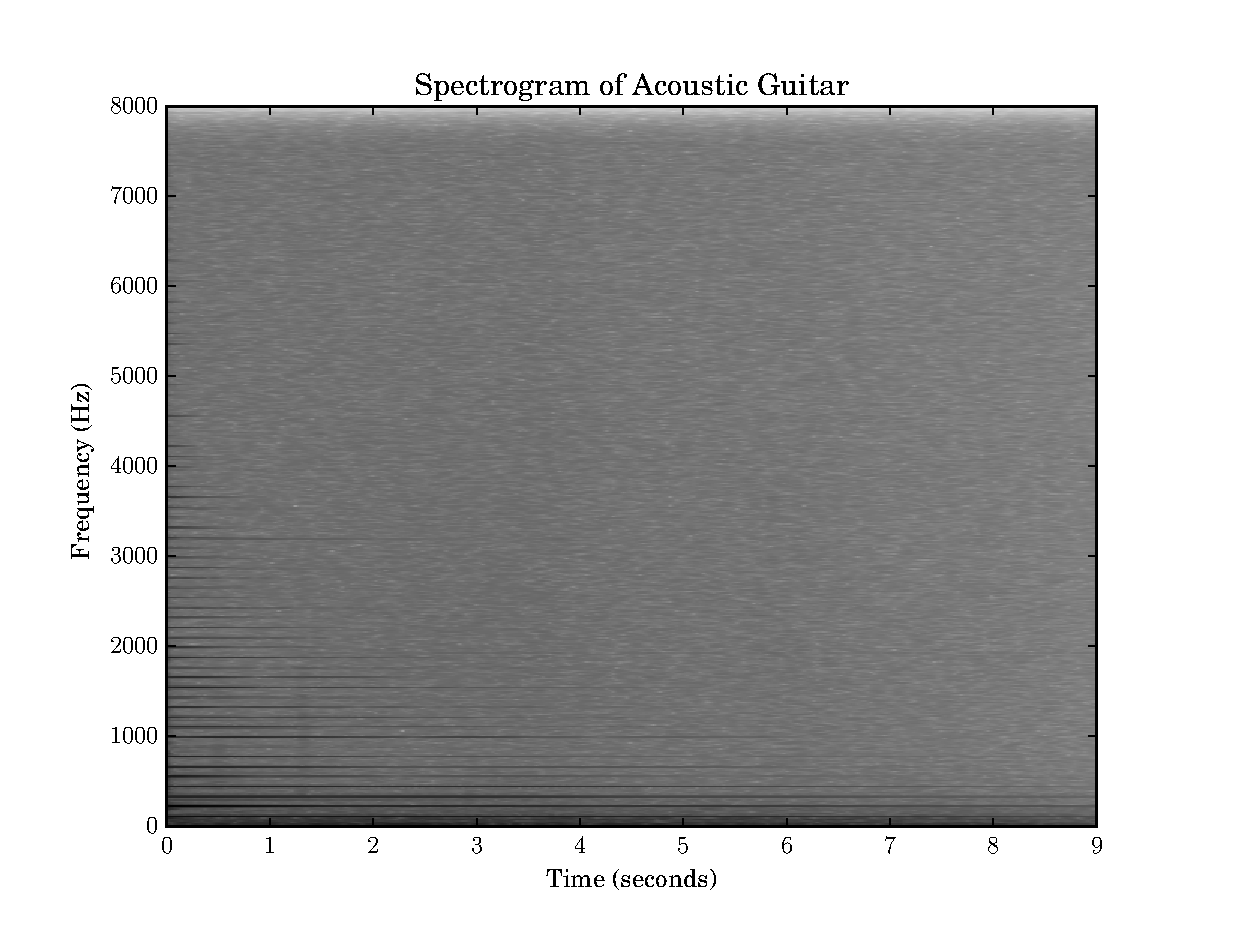
\includegraphics[width=\figwidthscale\textwidth]{plots/ac_gtr_orig_spec.eps}
    \CaptionWithTitle{%
        \input{plots/ac_gtr_orig_spec.txt}%
    }{The fundamental is $\text{A}_{3}$ or 220 Hz.%
    \label{plot:acgtra3specgram}}

    \vspace*{\floatsep}

    \centering
    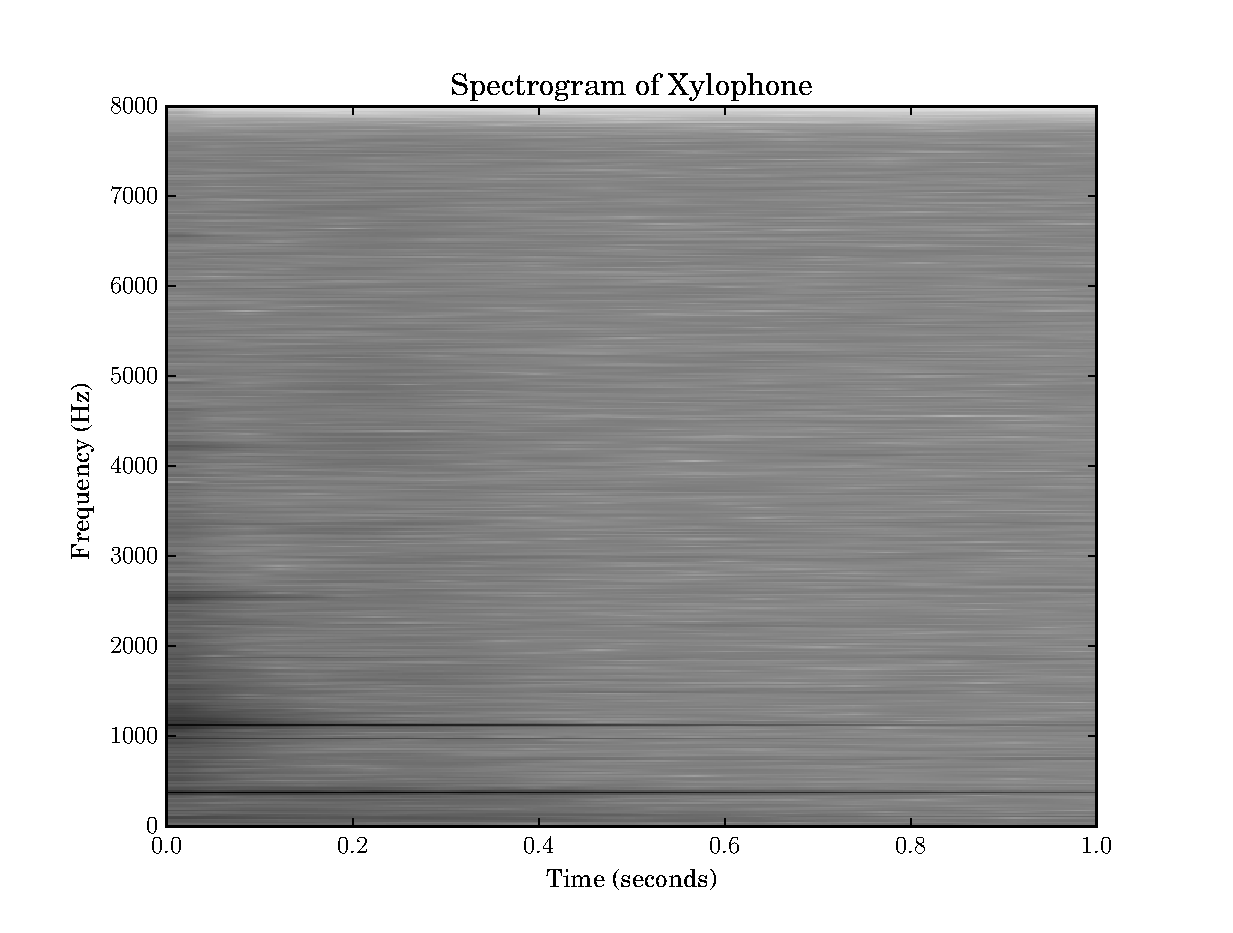
\includegraphics[width=\figwidthscale\textwidth]{plots/xylo_orig_spec.eps}
    \CaptionWithTitle{%
        \input{plots/xylo_orig_spec.txt}%
    }{The fundamental is $\text{F}_{4}^{\sharp}$ or approximately 370 Hz.%
    \label{plot:xylofs4specgram}}
\end{figure}

\begin{figure}[t]%[t]
    \centering
    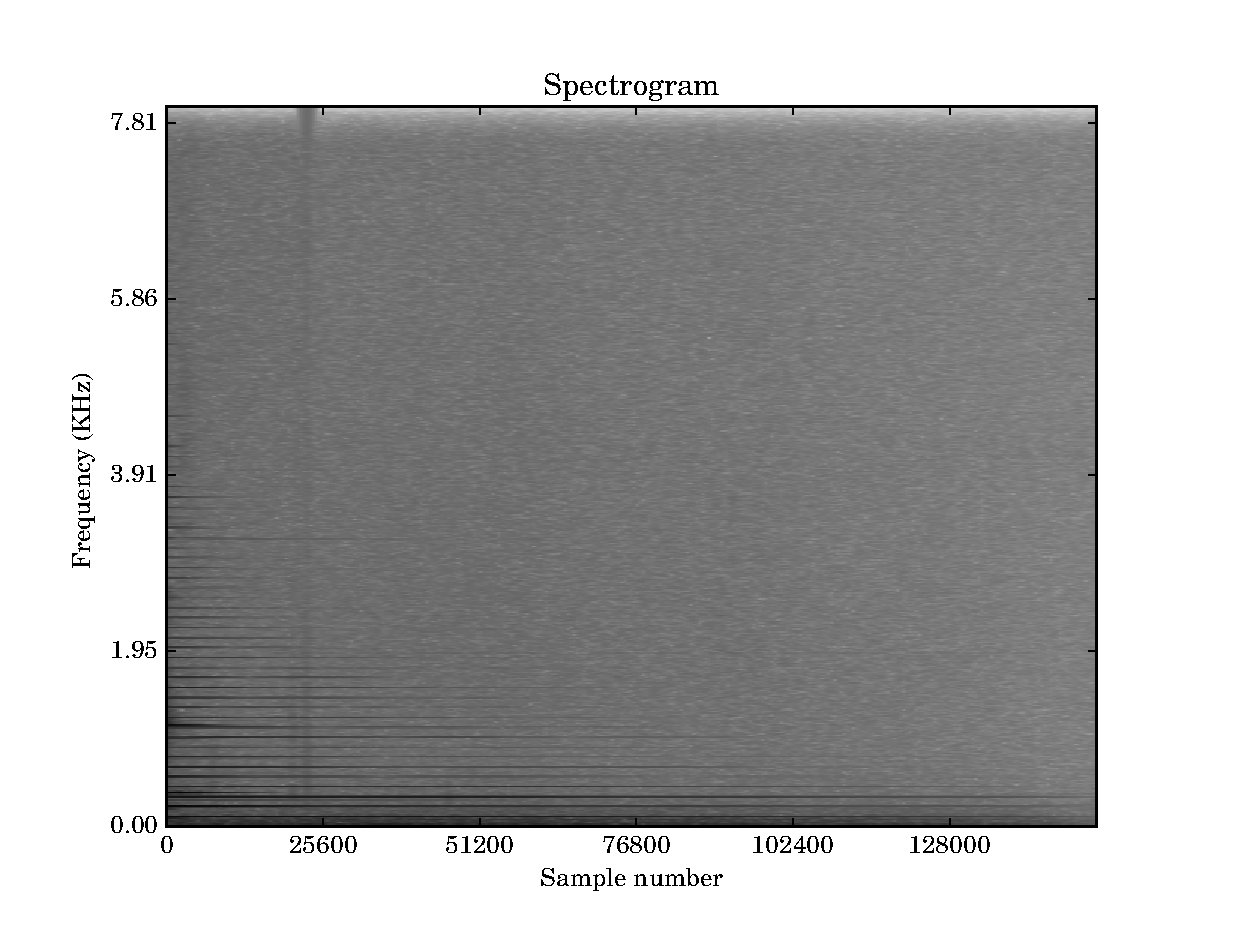
\includegraphics[width=\figwidthscale\textwidth]{plots/partial_estimation_acgtr_xylo_specgram.eps}
    \CaptionWithTitle{%
        \input{plots/partial_estimation_acgtr_xylo_specgram.txt}%
    }{This spectrogram is the sum of the spectrograms in
    Figure~\ref{plot:acgtra3specgram}~and~\ref{plot:xylofs4specgram}.%
    \label{plot:acgtra3xylofs4specgram}}
\end{figure}

We start with a recording of an acoustic guitar playing $\text{A}_{3}$ and
a xylophone playing $\text{F}_{4}^{\sharp}$.  The recordings are from
\cite{opolko1987mcgill} and have been mixed down to one channel (by simply
adding the two signals together) and resampled at 16 kHz, coded simply as a
stream of 64-bit floating-point numbers. Spectrograms of the original signals
are shown in Figure~\ref{plot:acgtra3specgram} and
Figure~\ref{plot:xylofs4specgram}. The spectrograms were produced with a Hann
window, DFT size of 4096 samples and a hop size of 512 samples. We see that
neither source exhibits much frequency-modulation. The spectrogram of
the mixture can be seen in Figure~\ref{plot:acgtra3xylofs4specgram} and the
partial paths in Figure~\ref{plot:acgtra3xylofs4partials}.

\begin{figure}
    \centering
    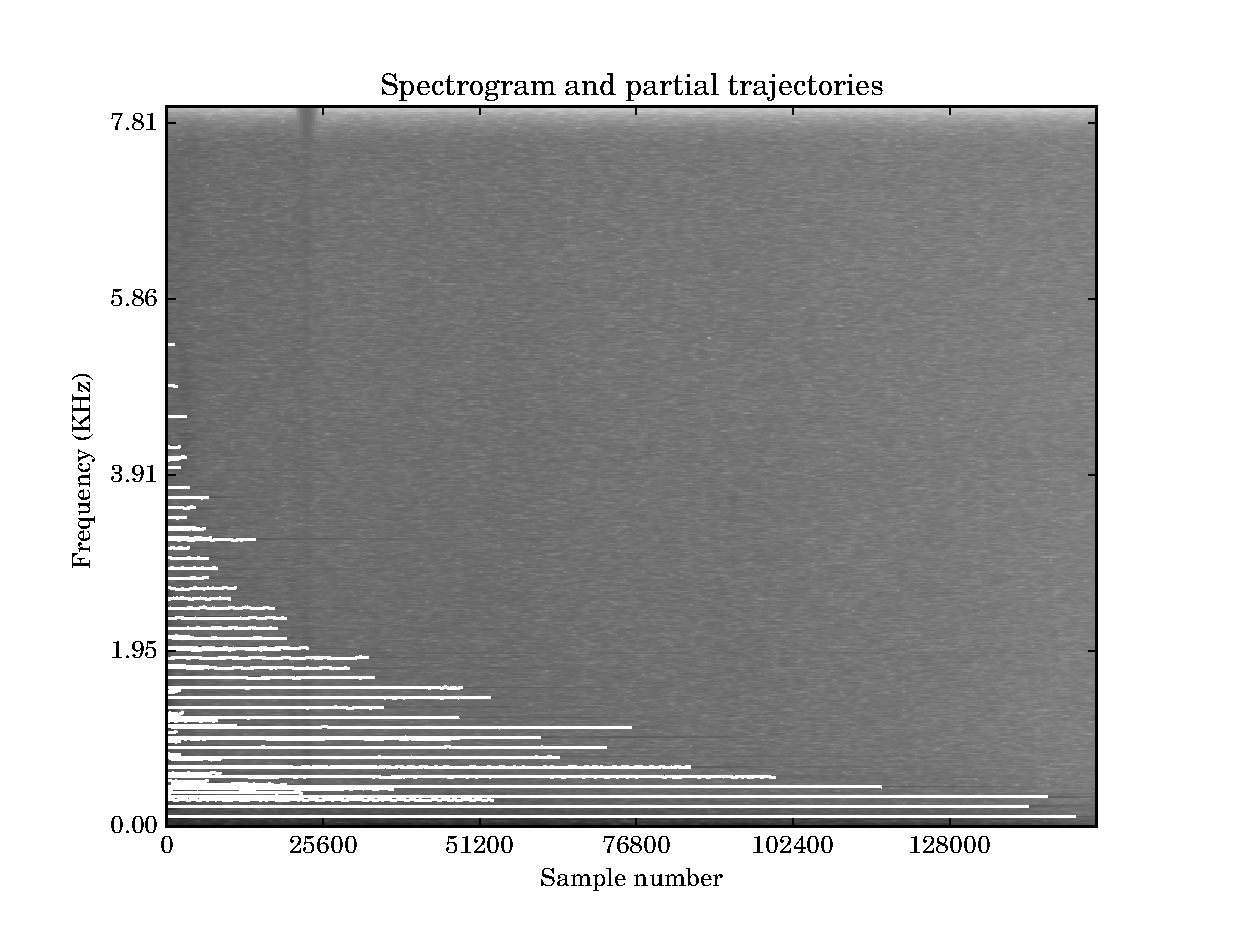
\includegraphics[width=\figwidthscale\textwidth]{plots/partial_estimation_acgtr_xylo_specgram_partials.eps}
    \CaptionWithTitle{%
        \input{plots/partial_estimation_acgtr_xylo_specgram_partials.txt}%
    }{\label{plot:acgtra3xylofs4partials}}

    \centering
    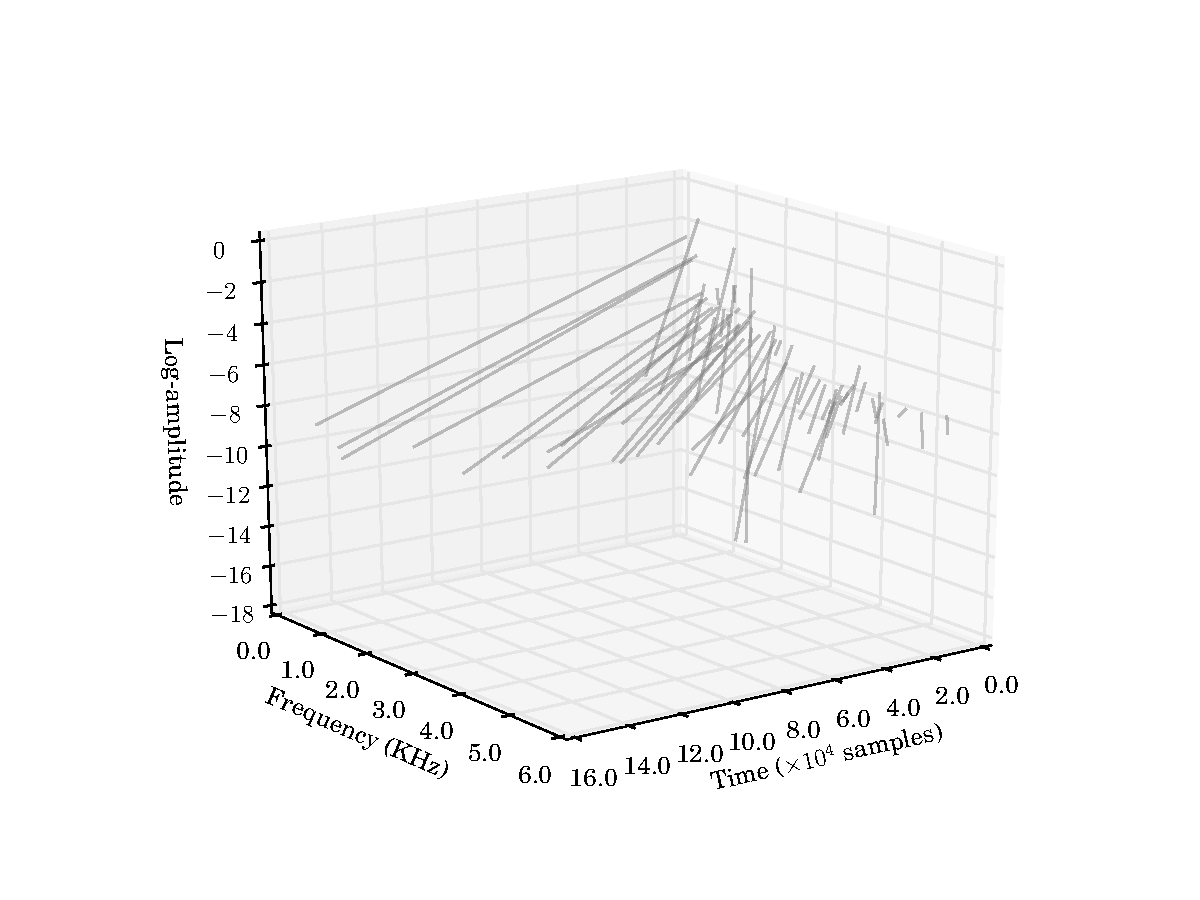
\includegraphics[width=\figwidthscale\textwidth]{plots/partial_classification_acgtr_xylo_partial_trajectories.pdf}
    \CaptionWithTitle{%
        \input{plots/partial_classification_acgtr_xylo_partial_trajectories.txt}%
    }{Line functions are fit to the partial trajectory data of each partial to
    examine their general amplitude slopes.%
\label{plot:parclassaxpartialtrajectories}}
\end{figure}

The mixture of the two signals was analysed using the DDM for finding the
coefficients of a cubic complex phase polynomial. Local maxima in each frame
were found using the technique described in \cite[p.~42]{serra1989system}. For
each of these local maxima, the polynomial coefficients were estimated. The
analysis used the $\mathcal{C}^{1}$ 4-Term Blackman-Harris window that was
designed in Chapter~\ref{chap:sigmod}. To obtain
partials it was then necessary to connect the local maxima. As the partials of
these two sound sources are quite stable in frequency it sufficed to use the
Viterbi algorithm \cite{forney1973viterbi} and the cost metric
$\mathcal{D}_{\text{pr.}}$ from Section~\ref{sec:mq_lp_compare_chirp} to connect
local maxima in sub-bands of the spectrum. The cost function is simply the
Euclidean distance between the frequencies of two local maxima. Partial starting
points are considered in sub-bands of width 15 Hz and these sub-bands overlap by
7.5 Hz. A partial path starts on the first local maximum in the band exceeding
-100 dB and ends at the last maximum exceeding -100 dB. The path search
algorithm will also look ahead to further frames if no maximum is present in the
next frame. Because of this, sometimes unrealistic paths are discovered that
jump between spurious maxima. These are filtered out by discarding paths whose
cost-length ratio is excessive. See
Figure~\ref{plot:acgtra3xylofs4costlengththresh} to see a plot of these values
and the thresholding function. 

\begin{figure}[t]
    \centering
    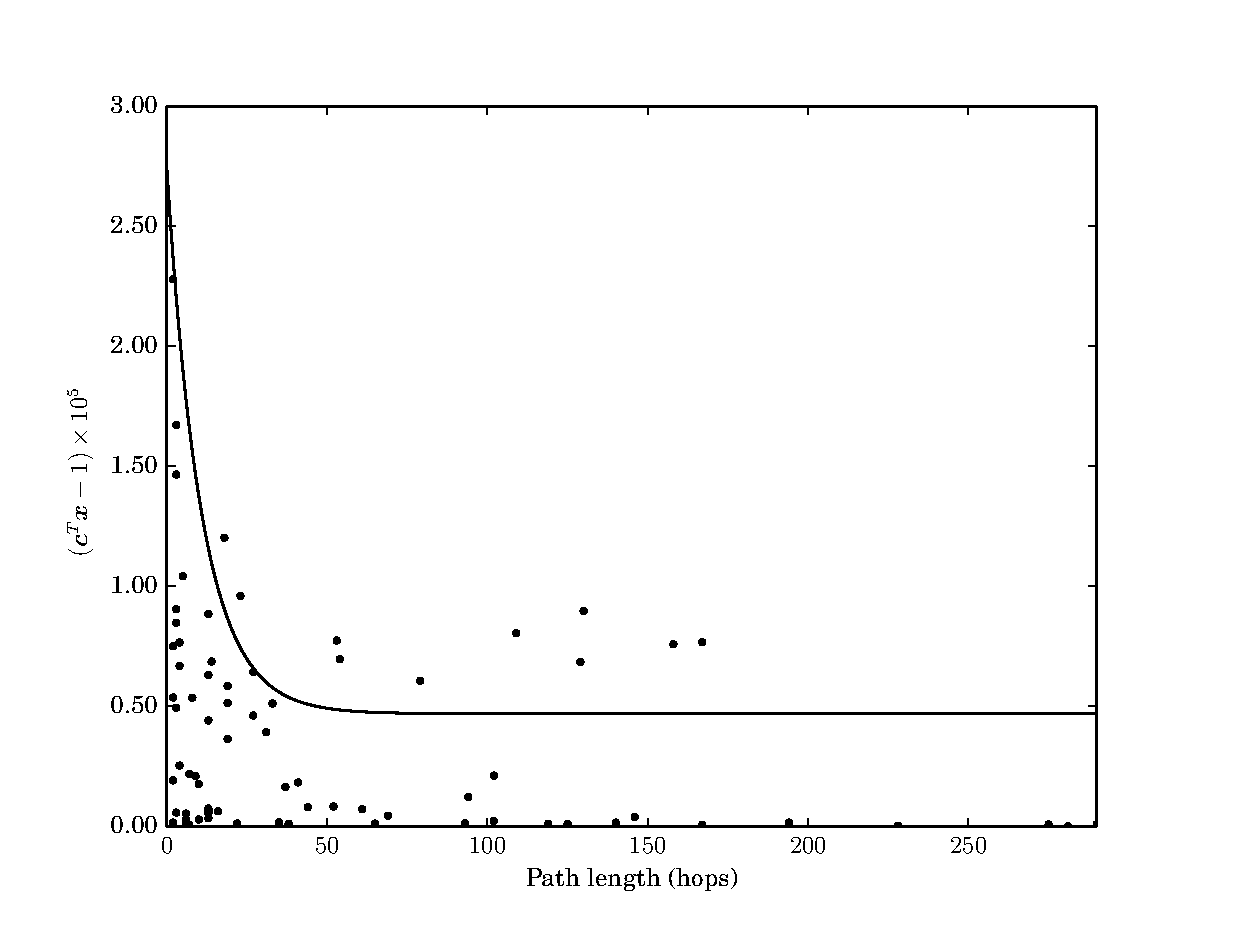
\includegraphics[width=\figwidthscale\textwidth]{plots/partial_estimation_acgtr_xylo_pcost_vs_bound.eps}
    \CaptionWithTitle{%
        \input{plots/partial_estimation_acgtr_xylo_pcost_vs_bound.txt}%
    }{Paths, represented as circles, are considered only if their
    path cost is smaller than the threshold function, the black curve. The
threshold is higher for shorter partials as to not reject those that
represent the transient region of the sound. The partials during this time
typically have rapidly changing frequency- and amplitude-modulation, so
their path costs could be disproportionately high.%
\label{plot:acgtra3xylofs4costlengththresh}}
\end{figure}

\section{Motivation}

\begin{figure}[t]
    \centering
    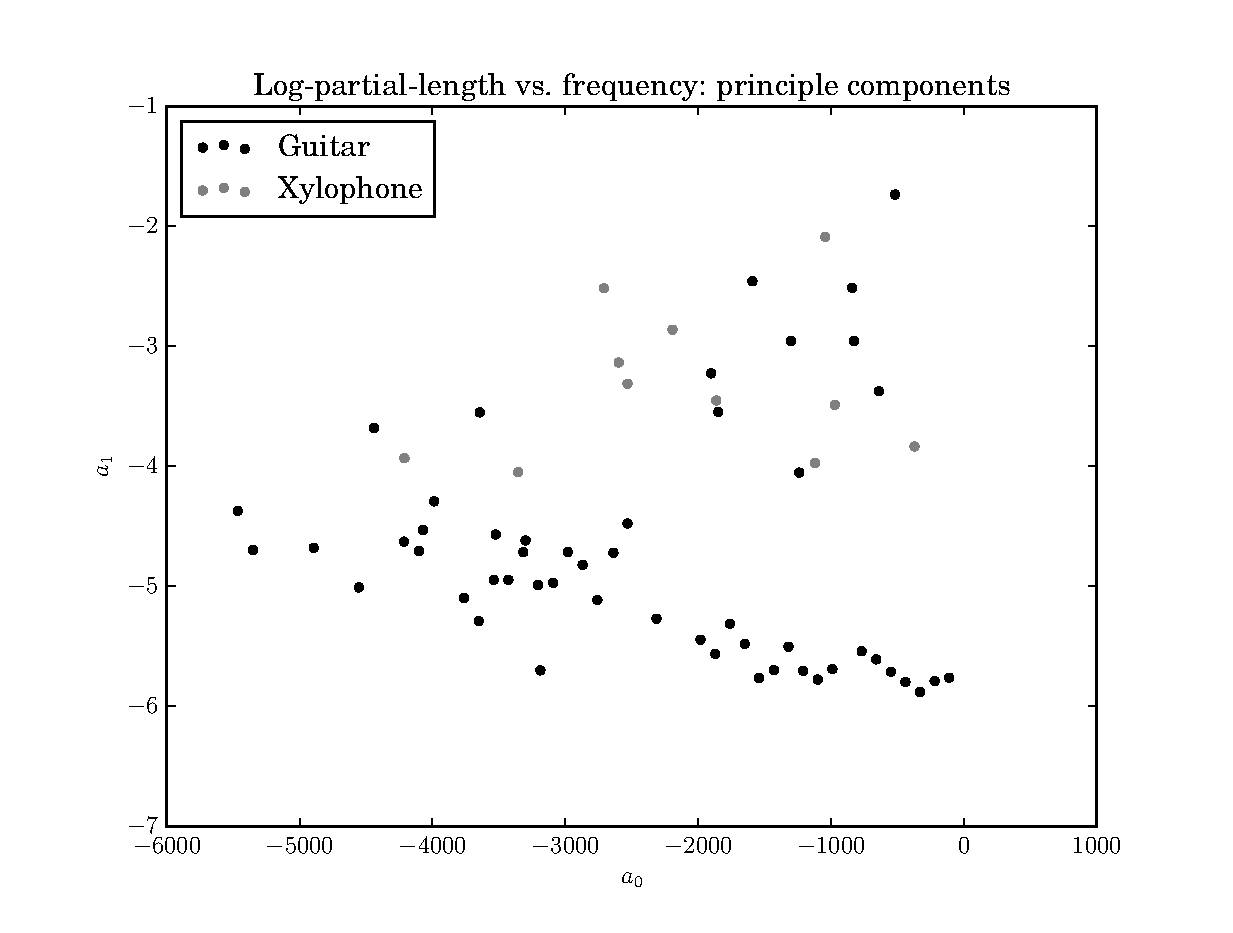
\includegraphics[width=\figwidthscale\textwidth]{plots/partial_classification_acgtr_xylo_sep_true_memberships.eps}
    \CaptionWithTitle{%
        \input{plots/partial_classification_acgtr_xylo_sep_true_memberships.txt}%
    }{This shows the distribution of partials when plotting their two principal components
        derived from their mean frequency and log-length. In this case, the
        source memberships of the partials are known. We see that there is
        generally a separation of the partials into two clusters corresponding
        to the two sources.
        \label{plot:partialclassificationacgtrxyloseptruememberships}}
\end{figure}

Line functions (functions of time) are fit to the amplitude and frequency data
on each partial trajectory via least-squares, as shown in
Figure~\ref{plot:parclassaxpartialtrajectories}. Here roughly two kinds of
partial slope with respect to amplitude are observed --- those that are steep and brief and
others that are longer and more gradual. Our goal is to classify based
on the amplitude modulation of each partial, or to an approximation, the slope
of these line functions. We found that examining the log-length of the partials
gives better results than examining the slope directly. This is perhaps
because the log-length encodes both the starting amplitude and the slope. Recall
that the partials start on the first local maximum exceeding an amplitude
threshold --- those with lower starting amplitude and steeper amplitude slope will be
shorter, while those with a higher starting amplitude and shallower slope will
be longer. We see in
Figure~\ref{plot:partialclassificationacgtrxyloseptruememberships} that using
both the amplitude-slope and the initial amplitude of the partial gives clear
separation in a plot of the log-length vs.\ the
average frequency of
the partials. These partials are from separate overlaid analyses of the guitar
and xylophone signals. The experiment uses an analysis of a signal consisting of
a mixture of the sources, of course.

The data-points have the form
\[
    \boldsymbol{a}_i = \begin{pmatrix}
        a_{i,0} \\
        a_{i,1}
    \end{pmatrix}
\]
where $a_{i,0}$ is the first principal components and $a_{i,1}$ the second and are computed via a
linear transformation of
\[
    \boldsymbol{x}_i
    =
    \begin{pmatrix}
        \overline{f}_{i} \\
        \ell_{i}
    \end{pmatrix}
\]
where $\overline{f}_{i}$ is the mean frequency of the $i$th partial and
$\ell_{i}$ its log-length (see
Appendix~\ref{chap:pca} for the computation of principal components). The set of
principal components will be denoted $\{\boldsymbol{a}\}$.
We see that, for the most part, the partials belonging to the two sources are
separated appropriately into two clusters. The partials from the xylophone
present in the guitar cluster belong to higher partials, whose omission in the
final rendering of the xylophone source would not be detrimental to its
perceptual quality. Similarly, partials belonging to the guitar present in the
xylophone cluster are short and most likely belong to briefly excited modes
of the guitar body.

\section{Classification}

Our intention is now to use GMM (see Appendix~\ref{chap:gmm}) on a set of
unclassified partials to yield a plausible source separation. GMM fitting is
sensitive to its initial guess of the parameters as the algorithm can converge
to a local maximum of the likelihood function
\cite[p.~187]{kay1993fundamentals}.  To find an initial guess we convolve the
scatter plot with kernel $\mathscr{K}$, giving a continuous function.
$\mathscr{K}$ is defined%
\footnote{Note its similarity to the normal distribution, defined in
Appendix~\ref{chap:normaldist}.}
\[
    \mathscr{K}(\boldsymbol{x},\boldsymbol{\beta})
    =
    \exp(\D-\frac{1}{2}\boldsymbol{x}^{T}\boldsymbol{\beta}^{-1}\boldsymbol{x})
\]
Here $\boldsymbol{x} \in \mathbb{R}^{2}$ and $\boldsymbol{\beta} \in
\mathbb{R}^{2 \times 2}$ controls the extent of the kernel, i.e., how much it
smooths in each dimension. 

\begin{figure}[t]%[!t]
    \centering
    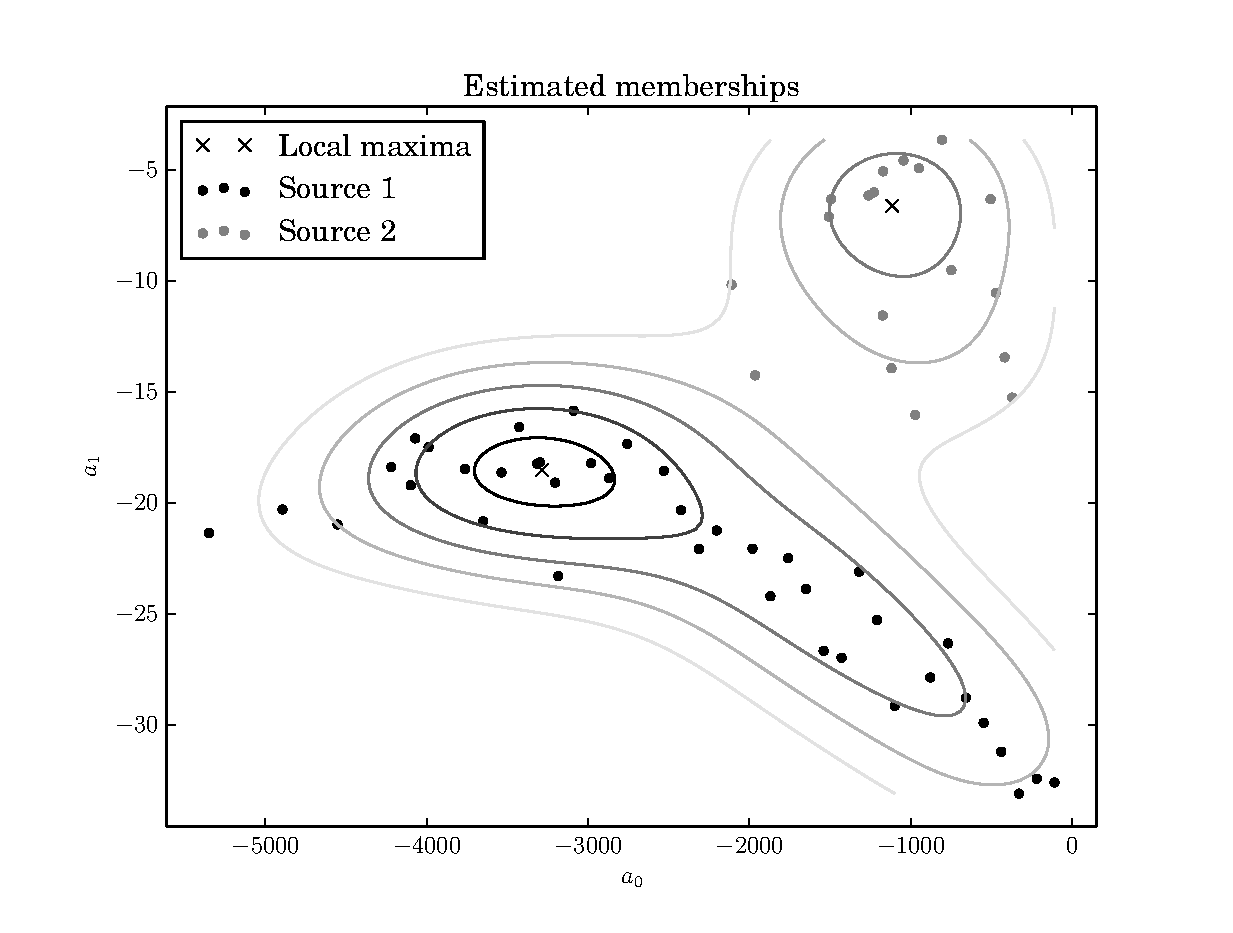
\includegraphics[width=\figwidthscale\textwidth]{plots/partial_classification_acgtr_xylo_estimated_memberships.eps}
    \CaptionWithTitle{%
        \input{plots/partial_classification_acgtr_xylo_estimated_memberships.txt}%
    }{The contours of the function resulting from convolving the data-points with kernels are
        represented by the lines. It is from the local maxima of these functions
        that the EM algorithm begins its search for the mixture of Gaussians
        (not shown) that give the classifications. A marker's classification is
        indicated by its colour.%
    \label{plot:partialclassificationacgtrxylosepestimatedmemberships}}
\end{figure}

We use the two local maxima of this function as the initial means for the two
sought classifying Gaussian distributions. The convolution function evaluated
at $\boldsymbol{\hat{a}}$ is
\[
    f(\boldsymbol{\hat{a}}) = \sum_{\boldsymbol{a}_i \in \{\boldsymbol{a}\}}
    \mathscr{K} \left( \boldsymbol{\hat{a}} - \boldsymbol{a}_i,
    \boldsymbol{\beta}_{\boldsymbol{a}} \right)
\]
To make the variance proportional to the extent of each dimension,
$\boldsymbol{\beta}_{\boldsymbol{a}}$ is defined as
\[
    \boldsymbol{\beta}_{\boldsymbol{a}}
    =
    \begin{pmatrix}
        \frac{\D\Delta_{\boldsymbol{a}_1}}{\D\Delta_{\boldsymbol{a}_0
        +\Delta_{\boldsymbol{a}_1}}}
            \theta_{\boldsymbol{\beta}_{\boldsymbol{a}}}
        & 0 \\
        0 & \frac{\D\Delta_{\boldsymbol{a}_0}}{\D\Delta_{\boldsymbol{a}_0
    +\Delta_{\boldsymbol{a}_1}}}
            \theta_{\boldsymbol{\beta}_{\boldsymbol{a}}}
    \end{pmatrix}
\]
where
\[
    \Delta_{\boldsymbol{a}_0} = \max \left( \boldsymbol{a}_0 \right)
        - \min \left( \boldsymbol{a}_0 \right)
\]
\[
    \Delta_{\boldsymbol{a}_1} = \max \left( \boldsymbol{a}_1 \right)
        - \min \left( \boldsymbol{a}_1 \right)
\]
and $\theta_{\boldsymbol{\beta}_{\boldsymbol{a}}}$ is a parameter to control
the smoothness of the resulting function, here
$\theta_{\boldsymbol{\beta}_{\boldsymbol{a}}} = 1.2$. A contour plot of the
resulting function $f(\boldsymbol{\hat{a}})$ is shown in
Figure~\ref{plot:partialclassificationacgtrxylosepestimatedmemberships}.

To initialize GMM the initial means $\boldsymbol{\mu}^{0}$ are chosen to be the
points corresponding to the local maxima of the smoothed scatter plot%
\footnote{Recall that the superscript here refers to the iteration number of the
algorithm.}. To
determine initial weights $\boldsymbol{w}^{0}$ we first determine the value of
the function at the two local maxima, $f(\boldsymbol{a}_{0}^{\ast})$ and
$f(\boldsymbol{a}_{1}^{\ast})$. To weight relative to these two values, we
compute
\[
    w_{i}^{0} = \frac{\Theta_{w} \left\{ f(\boldsymbol{a}_{i}^{\ast}) \right\}}{
    \sum_{p=0}^{R-1}\Theta_{w} \left\{ f(\boldsymbol{a}_{p}^{\ast} \right\}}
\]
where $\Theta_{w}$ is some kind of weighting operator to have parametric control
over the influence of each function value and $R$ is the number of maxima. Here
\[
    \Theta_{w} \left\{ f(\boldsymbol{a}_{i}^{\ast}) \right\}
    = \begin{cases}
        f(\boldsymbol{a}_{i}^{\ast}) \theta_{w} & i = 0 \\
        f(\boldsymbol{a}_{i}^{\ast}) & \text{otherwise}
    \end{cases}
\]
and $R = 2$, i.e., only the first maximum is weighted. For this experiment the parameter set as $\theta_{w} = 1.1$ gave
the best results. The covariance matrix $\boldsymbol{\Sigma}^{0}$ is computed as
\[
    \boldsymbol{\Sigma}^{0} = \boldsymbol{S}(\{ \boldsymbol{a} \}) +
    \epsilon\boldsymbol{I}
\]
\begin{figure}[t]
    \centering
    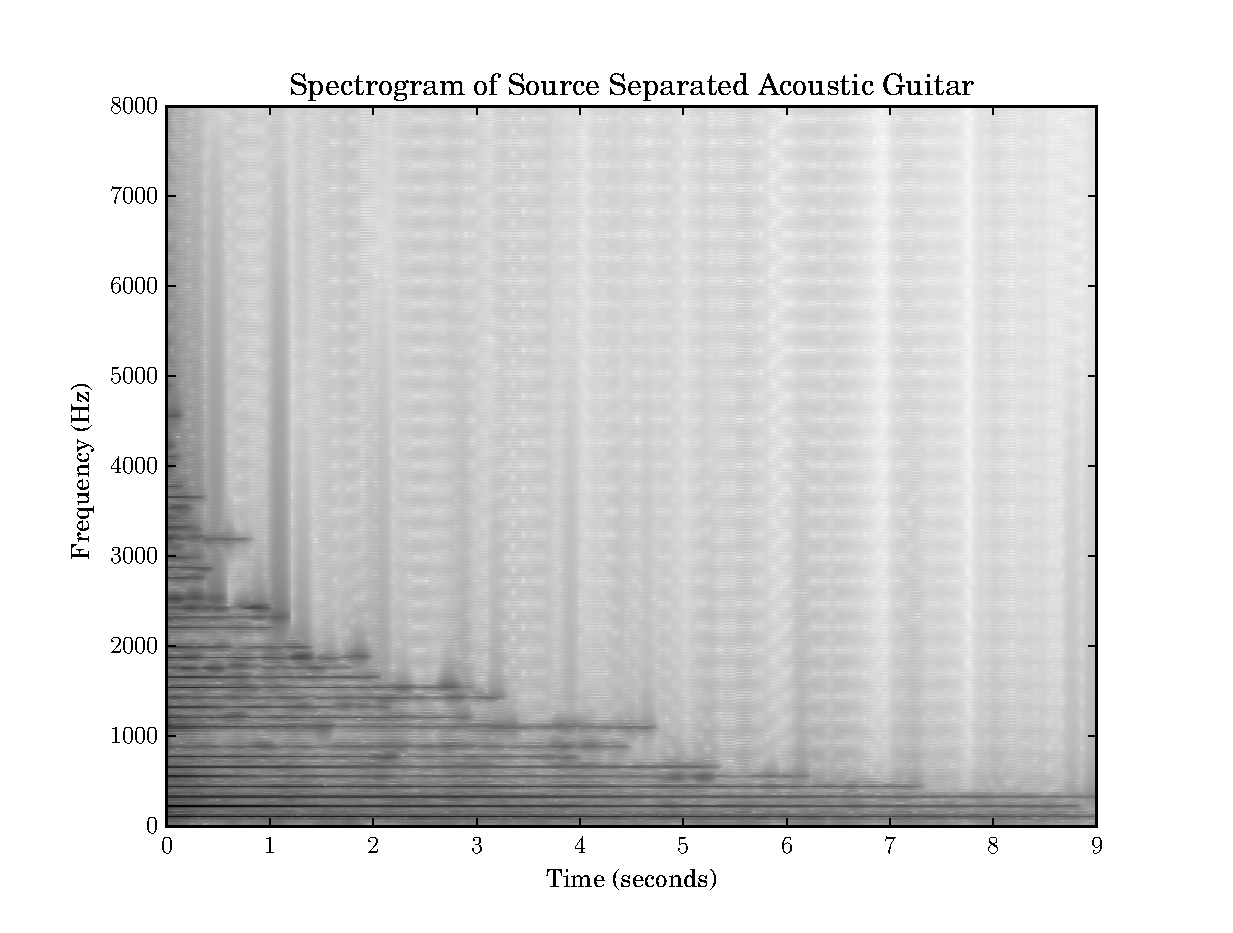
\includegraphics[width=\figwidthscale\textwidth]{plots/ac_gtr_ss_spec.eps}
    \CaptionWithTitle{%
        \input{plots/ac_gtr_ss_spec.txt}%
    }{\label{plot:acgtra3specgramss}}
\end{figure}%
where $\boldsymbol{S}$ computes the sample covariance and
$\boldsymbol{\epsilon}\boldsymbol{I}$ is a matrix whose only non-zero entries
are on the main diagonal and are equal to a small constant to avoid a singular
initial covariance matrix. 100 iterations of the EM algorithm (see
\ref{chap:gmm}) are performed to compute classifications. Each point is assigned
to its most likely cluster using the final estimated Gaussian distributions. The
final classifications for this classification task can be seen in
Figure~\ref{plot:partialclassificationacgtrxylosepestimatedmemberships}.

\section{Synthesis}

After the classifications have been made, synthesizing the separated sources
simply involves only synthesizing the partials classified as belonging to the
same source. For the synthesis, we use the technique described in
Section~\ref{sec:s23synthesis}. Spectrograms of the source separated signals
are shown in Figure~\ref{plot:acgtra3specgramss} and
Figure~\ref{plot:xylofs4specgramss}. 

\begin{figure}[t]
    \centering
    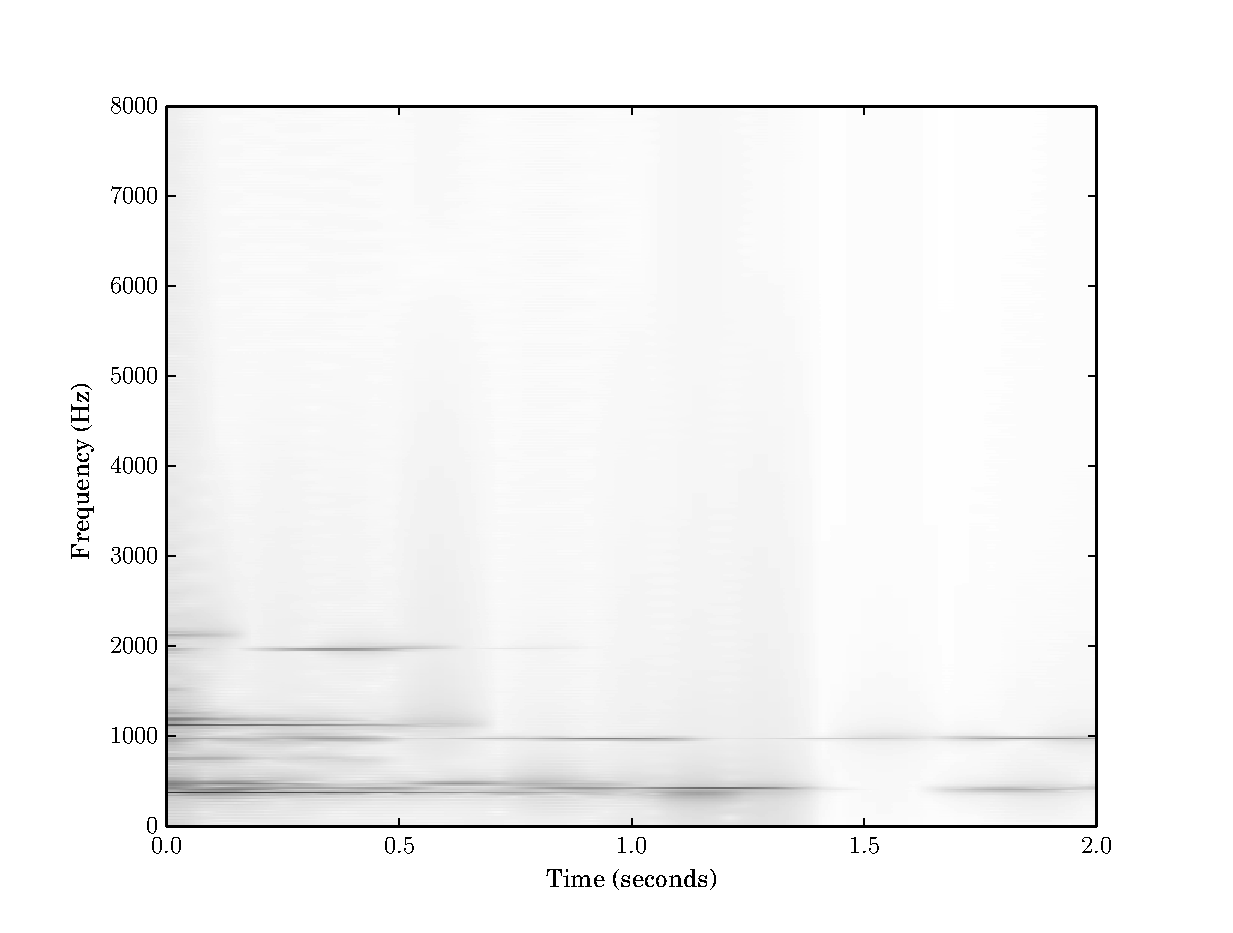
\includegraphics[width=\figwidthscale\textwidth]{plots/xylo_ss_spec.eps}
    \CaptionWithTitle{%
        \input{plots/xylo_ss_spec.txt}%
    }{\label{plot:xylofs4specgramss}}
\end{figure}

\section{Conclusion}

After an informal listening, the source separation is perceptually
convincing.\footnote{Soundfiles can be downloaded from \par
\url{https://drive.google.com/file/d/0B8B4c04j8tBwZDFraEZ1dFZHRFU/view?usp=sharing}}
At least one partial from the guitar can be heard in the xylophone recording,
however --- it is difficult to separate partials that do not have sufficient
spatial separation in
Figure~\ref{plot:partialclassificationacgtrxylosepestimatedmemberships}. Another
drawback of the current technique is that it requires some tuning of the
parameters $\theta_{w}$ and $\theta_{\boldsymbol{\beta}_{\boldsymbol{a}}}$.
From the spectrograms of the resynthesized sources, we see that some of the
partials from both sounds were lost in the analysis.  Although a shortcoming of
the analysis rather than the classification, if partials are not sufficiently
separated in time or frequency, they cannot be separated as their analysis will
yield simply one partial when there are in fact many. In any case, it is important
to see that source separation can be carried out by only considering the
amplitude modulation (in this case, the decay rate) in relation to the partial
frequency. Apart from the combination of instruments presented here many
plausible situations can be imagined where this technique could be carried out:
e.g., with a mixture of sustained instruments such as violin, voice or horns and
pitched percussive instruments such as the piano or guitar.


\chapter{Conclusion\label{chap:conclusion}}

Here we summarize the results of our work, highlight our contributions to the
audio source separation problem, and suggest some possible extensions to the
techniques presented in this thesis.

\section{Results}

\subsection{Quality of polynomial models for analysis and synthesis}

In Chapter~\ref{chap:exphsmodel} we explored various orders of polynomial amplitude and
phase models for analysis and synthesis and assessed their fidelity in
reproducing synthetic signals of with polynomial and exponential phase functions. A
quadratic estimation of the phase and log-amplitude in the analysis step
improved the synthesis quality over the constant amplitude and linear phase
model in all cases considered. The use of a quintic phase
polynomial in the synthesis step better approximated a signal with exponential
phase. However, the use of the quintic phase and amplitude polynomial did not
necessarily improve the synthesis of a signal with cubic phase and quartic
amplitude. Nevertheless, the additional information provided by the DDM in the
analysis stage was shown useful in postulating interpolating polynomials at the
synthesis stage.

\subsection{The use of amplitude- and frequency-modulation in audio source separation}

Chapter~\ref{chap:amfmsep} explored the contribution of amplitude- and
frequency-modulation to the source separation problem on simulated data.
Chapter~\ref{chap:decaysep} investigated, using real recordings, how to overcome
the case where no frequency-modulation was present in either of the sources and
so only amplitude-modulation could be used to perform separation.

\subsubsection{Using amplitude- and
frequency-modulation}

In Chapter~\ref{chap:amfmsep} we considered both the amplitude- and
frequency-modulation when classifying into sources. We adaptively selected the
best variable on which to classify using principal components analysis and found
that amplitude-modulation aided in the case of little frequency-modulation. A
post-processing step was required to extract the original sources. This step
extracted sources based on the smoothness between analysis frames of the
amplitude and frequency measurements.  Only the post-processing encouraging
smoothness in frequency gave encouraging results --- smoothing in amplitude
failed due to the rapidly varying amplitude in the transient regions of the
sounds.

\subsubsection{Real recordings with no
frequency-modulation}

In Chapter~\ref{chap:decaysep} we applied our source separation technique
to a recording of a percussive and a plucked string instrument. These
instruments exhibit virtually no frequency-modulation. We showed, as in
Chapter~\ref{chap:amfmsep}, that it is
possible to carry out source separation when the difference in
amplitude-modulation of the two sources is sufficient. 

\section{Contributions}

\subsection{Design of continuous windows with lower side-lobes}

The DDM requires the use of windows that are once differentiable. The canonical
window with this property is the Hann window, however the Blackman-Harris window
has better properties in terms of its out-of-band signal rejection, but is not
differentiable. In
Chapter~\ref{chap:sigmod}, starting
from the description of a Blackman-Harris window, we used optimization
techniques to search for a window close to the Blackman-Harris, but whose
end-points are 0, thus allowing differentiation everywhere after windowing with
a rectangular window (necessary to make the window have finite support).
Although no formal quantification of the improvement was performed, we found
this to improve the estimation accuracy of the DDM for signals sufficiently
separated in frequency (separated by at least the bandwidth of the main-lobe of
the frequency domain representation of the window) when compared with the DDM
using the Hann window.

\subsection{Partial tracking using linear programming}

The original peak-matching algorithm of McAulay and Quatieri
\cite{mcaulay1986speech} searches for partials through a lattice of spectral
analysis data by considering optimal peak-matches between two adjacent frames.
In Chapter~\ref{chap:partialtracking} we show that this can be generalized to
search for $L$ paths between an arbitrary number of frames in a lattice, and
that it is a greedy algorithm --- one that gives the shortest possible path
without considering the lengths of the other paths in the solution. Also, it is
shown that the complexity of this algorithm is exponential in the number of
frames and therefore impractical to apply to even moderately sized problems. A
linear program to search for the $L$ paths through a lattice with shortest total
cost is introduced. We show that this algorithm is computationally tractable and
that it outperforms the McAulay-Quatieri method on signals with low SNRs.

\section{Future extensions}

\subsection{Continuous analysis windows}

It remains to be seen systematically in what situations the continuous
Blackman-Harris window improves the estimation accuracy of the DDM. For this,
DDM-based analysis using both the Hann and continuous Blackman-Harris windows
should be performed on mixtures of synthetic signals and the accuracy of
analysis compared. Further improvements to the window design could be
investigated, such as finding a continuous Blackman-Harris window with good
trade-off between main-lobe width and side-lobe height.

\subsection{Partial tracking in an optimization framework}

The reinterpretation of partial tracking as an optimization problem allows the
application of techniques from mathematical programming, a field with
a rich body of knowledge \cite{boyd2004convex}. As discussed in
Chapter~\ref{chap:partialtracking}, regularization could be used to encourage
less ``jagged'' partial trajectories. The merits of partial tracking via
linear programming should be assessed on real music and speech signals.

\subsection{Signal modeling with nonlinear amplitude and phase polynomials}

A non-stationary description of signals could make it possible to describe
signals using fewer analysis frames as the signal can be more accurately modeled
between analysis points. As mentioned in \cite{betser2009sinusoidal}, it should
be investigated whether or not such a model could contribute to the field of audio
coding. Specifically, compression ratios should be compared between analyses
using a lower-order model, but with more analysis frames, and those using higher-order
models but fewer analysis frames. Possible improvements to applications such as
the time-stretching of transients and the extrapolation of missing signals
(inpainting) should also be considered.


\begin{appendices}

    \chapter{Principal components analysis (PCA)}

\section{Motivation}

If data-points consist of more than two dimensions (say $p$), it becomes
burdensome to try and find the single best or two best dimensions on which to
examine for grouping. If we consider variables on each of the dimensions that
take on the data-point's corresponding values, we are interested in the
variables that capture most of the data-points's variance. In turns out we can
determine a linear transformation of our original dataset giving $p$ variables
and their $p$ variances such that the resulting variable with the highest
variance will have the maximum variance acheivable, under some constraints that
will be explained shortly. 

\section{Computation of principal components}

The following development is based on \cite{jolliffe2002principal}. Say we have
a set $\left\{ \boldsymbol{x} \right\}$ of data-points and their covariance
matrix $\boldsymbol{S}$. A linear function of $\boldsymbol{x}$,
$f_1(\boldsymbol{x})=\boldsymbol{a}_{1}^{T}\boldsymbol{x}$ has variance
$\sigma_{\boldsymbol{a}_{1}^{T}\boldsymbol{x}}=\boldsymbol{a}_{1}^{T}\boldsymbol{S}\boldsymbol{a}_{1}$.
Therefore, we desire a vector $a$ that maximizes
$\sigma_{\boldsymbol{a}_{1}^{T}\boldsymbol{x}}$. We can find this via the program
\[
        \max \boldsymbol{a}_{1}^{T}\boldsymbol{S}\boldsymbol{a}_{1}
\]
subject to
\[
    \boldsymbol{a}_{1}^{T}\boldsymbol{S}\boldsymbol{a}_{1}=1
\]
(to obtain a bounded solution).

The resulting function of $\boldsymbol{x}$,
$f_1(\boldsymbol{x})=\boldsymbol{a}_{1}^{\ast T}\boldsymbol{x}$ is called the first
\textit{principal component}. The second principal component
$f_2(\boldsymbol{x})=\boldsymbol{a}_{2}^{\ast T}\boldsymbol{x}$ is found similary
to the first, except with the additional constraint that it be uncorrelated
(orthogonal) to the first component, i.e.,
$\boldsymbol{a}_{2}^{\ast T}\boldsymbol{a}_{1}=0$, and the third is found by
requiring orthognality with the first two principal components, etc.

The principal components (PCs) now allow us to examine for grouping more easily as the
total variance of the dataset has been captured in the first few principal component
variables. These transformed data-points can now be classified using a
classification algorithm.

Before we continue describing classification techniques we will briefly discuss
the nature of our classification problem. If accurate and consistent
measurements of data-points can be made, and a large enough sample of
data-points is available to train a model, then to predict the classification of
new points, a function $g=\hat{h} \left( \boldsymbol{x} \right)$ is postulated,
giving the classification $g$ of a data-point $\boldsymbol{x}$. For example, if
there are only two classes, we might postulate a linear
classifier
\[
    \hat{h}(\boldsymbol{x}) = \begin{cases}
        0 \text{ if } \boldsymbol{\beta}^{T}\boldsymbol{x} > c \\
        1 \text{ if } \boldsymbol{\beta}^{T}\boldsymbol{x} < c
    \end{cases}
\]
where 0 and 1 indicate membership in class 0 or 1. Techniques for choosing
$\hat{h}$ are discussed in \ref{friedman2001elements} and often require data on
which to ``train'' a classifier, i.e., determine a function $\hat{h}$ that
classifies well a dataset with known classifications.  Here we do not have a
sample dataset because of the large number of possible situations and the
difficulty of consistently estimating underlying model parameters (see, for
example, Section~\ref{sec:mq_lp_compare_chirp}). As training to find a suitable
$\hat{h}$ is not possible, we propose \textit{kernels} that reflect the
hypothesized underlying structure of the distribution of $\boldsymbol{x}$. To
elaborate, we may observe that the classification of a
point is indicated by its nearness to other points in the same class, i.e., its
membership to a cluster. The proposed kernel is a parameterized model of a
cluster, whose parameters we can adjust until they fit the observed data well.
We then choose the kernel that best explains the data to indicate what class
these data are in. The following section describes a technique using normal
distributions as kernels, which is the technique used in later experiments.


    \chapter{Gaussian mixture models (GMM) \label{chap:gmm}}

Consider the data-points $\boldsymbol{X}$ as realizations of the vector Gaussian
distributed random variable $X$. With a large enough sample and a small enough
covariance, we will observe realizations of $X$ as a cluster with some mean
(centre point) $\boldsymbol{\mu}$ and a shape described by the covariance matrix
$\boldsymbol{\Sigma}$. If we observe multiple clusters this might imply that
there are $P$ different distributions each with mean $\boldsymbol{\mu}_p$ and
covariance matrix $\boldsymbol{\Sigma}_p$ and on each iteration one is chosen
with probability $w_p$. With $N$ observations $\boldsymbol{x}_{n}$ we can
estimate, via maximum likelihood, the $P$ sets of parameters using a form of the
\textit{expectation maximization (EM)} algorithm \cite{moon1996expectation},
\cite{dempster1977maximum}, which is an algorithm suitable for estimating
missing data from known ones. First, define
\[
    \mathrm{p} \left( \boldsymbol{x}_{n} | p \right)
    =
    \ddfrac{
        \mathcal{N} \left( \boldsymbol{x}_{n}; \boldsymbol{\mu}^{k}_{p} ,
        \boldsymbol{\Sigma}^{k}_{p} \right) w^{k}_{p}
    }{
        \sum_{l=1}^{P}
        \mathcal{N} \left( \boldsymbol{x}_{n}; \boldsymbol{\mu}^{k}_{l} ,
        \boldsymbol{\Sigma}^{k}_{l} \right) w^{k}_{l}
    }
\]
the probability that $\boldsymbol{x}_n$ given distribution $p$ (see
Appendix~\ref{chap:normaldist} for the definition of $\mathcal{N} \left(
\boldsymbol{x} ; \boldsymbol{\mu}^{k} , \boldsymbol{\Sigma}^{k} \right)$). The superscript $k$
indicates the value of this parameter on iteration $k$. To update $w^{k}_p$:
\[
    w^{k+1}_p = \frac{1}{N} \sum_{n=1}^{N} \mathrm{p} \left( \boldsymbol{x}_n |
    p \right)
\]
which means intuitively that the probability of a data-point having been
generated by distribution $p$ is the average probability of observing any
$\boldsymbol{x}_n$ given $p$. To update $\boldsymbol{\mu}^{k+1}_p$:
\[
    \boldsymbol{\mu}^{k+1}_p
    =
    \ddfrac{\sum_{n=1}^{N} \mathrm{p} \left( \boldsymbol{x}_n |
    p \right) \boldsymbol{x}_n }{\sum_{n=1}^{N} \mathrm{p} \left( \boldsymbol{x}_n |
    p \right)}
\]
which is a weighted mean of all the data-points. Those less likely for a
given $p$ will weight the mean less and vice versa. A similar computation is
made for $\boldsymbol{\Sigma}^{k+1}_p$:
\[
    \boldsymbol{\Sigma}^{k+1}_p
    =
    \ddfrac{\sum_{n=1}^{N} \mathrm{p} \left( \boldsymbol{x}_n | p \right)
        \left( \boldsymbol{x}_n - \boldsymbol{\mu}^{k+1}_p \right) \left(
        \boldsymbol{x}_n - \boldsymbol{\mu}^{k+1}_p \right)^{T}
    }{
        \sum_{n=1}^{N} \mathrm{p} \left( \boldsymbol{x}_n | p \right)
    }
\]
The algorithm is halted after some number of iterations or when convergence is
reached, i.e., the parameters change little each iteration. After convergence, the
classification $p^{\ast}$ of the data-point $\boldsymbol{x}$ is simply
\[
    p^{\ast} = \argmax_{p} \mathrm{p} \left( \boldsymbol{x}_n | p \right)
\]



    \chapter{The normal distribution\label{chap:normaldist}}

If a random variable $X$ is has mean $\mu = E(X)$ and variance $\sigma^{2} =
E((X-\mu)^{2})$, where $E$ is the expectation operator, and is completely
described by these two parameters, we say that draws from $X$, $x$, follow a
normal distribution. Put another way, given a draw $x$ from $X$, the probability of
obtaining $x$ is given by
\[
    \mathrm{p}_{\mathcal{N}}(x)
    =
    \mathcal{N}(x;\mu,\sigma^{2})
    =
    \frac{1}{\sqrt{2\pi\sigma^{2}}}\exp(-\frac{(x-\mu)^{2}}{2\sigma^{2}})
\]
When a random variable $X$ is distributed by a normal distribution with mean $\mu$
and variance $\sigma^{2}$ we write
\[
    X \sim \mathcal{N}(\mu,\sigma^{2})
\]
In the case that $\boldsymbol{\tilde{x}}$ is an $N$-dimensional random vector%
\footnote{We write $\boldsymbol{\tilde{x}}$ because $\boldsymbol{X}$ would be a
matrix.} characterized by
the multidimensional mean $\boldsymbol{\mu} = E(\boldsymbol{\tilde{x}})$ and
covariance matrix
$\boldsymbol{\Sigma} =
E((\boldsymbol{\tilde{x}}-\boldsymbol{\mu})(\boldsymbol{\tilde{x}}-\boldsymbol{\mu})^{T})$
then the probability of obtaining a realization $\boldsymbol{x}$ is given by
\[
    ((2\pi)^{N}|\boldsymbol{\Sigma}|)^{-1/2}%
    \exp(\D-\frac{1}{2}(\boldsymbol{x}-\boldsymbol{\mu})^{T}%
    \boldsymbol{\Sigma}^{-1}(\boldsymbol{x}-\boldsymbol{\mu}))
\]
$|\boldsymbol{\Sigma}|$ means the determinant of $\boldsymbol{\Sigma}$. Similar
to above, when a random vector is distributed by a normal distribution, we write
\[
    \boldsymbol{\tilde{x}} \sim \mathcal{N}(\boldsymbol{\mu},\boldsymbol{\Sigma})
\]
The normal distribution, also called the Gaussian distribution, arises
often in statistics and signal processing due to the \textit{Central Limit
Theorem} \cite{feller2008introduction} and its relationship to least-squares
estimation \cite{kay1993fundamentals}.


\end{appendices}

\cleardoublepage\phantomsection
\bibliographystyle{plain}
\bibliography{thesis}
\end{document}
